%*********************************
%Format telah disesuaikan sesuai *
%Panduan penulisan               *
%Disertasi Dan Tesis ITS         *
%*********************************
 \documentclass[12pt, a4paper,twoside, bahasa]{report}
%\documentclass[12pt, a4paper,twoside]{report}

\title{Buku Tesis}
% Jika pakai windows untuk run
%    pertama kali dan error.
% Mohon cek miktex console jika 
%    compiler latex nya menggunakan miktex.
%------------------------------
%%%%%%%%%%%%%%%%%%%%%%%%%%%%%%%%%%%%%%%%%%%%
% FILE INI JANGAN DI UBAH
%%%%%%%%%%%%%%%%%%%%%%%%%%%%%%%%%%%%%%%%%%%%
\usepackage[indonesian]{babel}
%\usepackage[indonesian]{babel}



\usepackage[pdfauthor={Rohman Widiyanto},bookmarksnumbered,pdfborder={0 0 0}]{hyperref}
\usepackage[ruled,lined,commentsnumbered,linesnumbered]{algorithm2e}
\usepackage[utf8]{inputenc}
\usepackage{graphicx}
\usepackage{lipsum}  
\usepackage{hyphenat}
\usepackage{rotating}
\usepackage{booktabs}
\usepackage{lscape}
%\usepackage{algpseudocode}
\usepackage[ruled,lined,commentsnumbered,linesnumbered]{algorithm2e}
\usepackage{algpseudocode}
\usepackage{makeidx}
\usepackage{rotating}
\makeindex
\usepackage{epsfig}
\usepackage{subfig}
\usepackage{pdflscape}
\usepackage[doublespacing]{setspace}
\setstretch{1.5}
\usepackage{type1cm}
\usepackage{longtable}
\usepackage{lscape}
\usepackage{lettrine}
\usepackage{hyperref}
\usepackage[pageref]{backref}
\usepackage{multirow}
\usepackage[table,xcdraw]{xcolor}
\usepackage{eso-pic}
\newcommand\BackgroundIm{
	\put(0,0){
		\parbox[b][\paperheight]{\paperwidth}{%
			\vfill
			\centering
			\includegraphics[height=\paperheight,
			keepaspectratio]{./lib/background.png}%
			\vfill
}}}

\usepackage{fancyhdr} % Untuk pengaturan header dan footer yang lebih kompleks
\usepackage{etoolbox} % Untuk melakukan perubahan (patch) command internal LaTeX
\usepackage{url}
\usepackage{longtable}
\usepackage{float}
\usepackage{morefloats}
\floatstyle{boxed}
\newfloat{program}{thp}{lop}
\floatname{program}{Program}
\usepackage[fleqn]{amsmath}
\usepackage{nccmath}
\usepackage{enumitem}
\usepackage{nonfloat}
\usepackage{ulem}
\usepackage[final]{pdfpages}
\usepackage{titlesec}
\usepackage{array}
\usepackage{multicol}
\usepackage{listings}
\usepackage{wrapfig}
\usepackage{array,tabularx}
\usepackage{lscape}
\usepackage{longtable}
\usepackage{caption}
\usepackage[export]{adjustbox}
\usepackage{ragged2e}
\usepackage{epsfig}
\usepackage{subfig}
\usepackage[top=35mm,left=40mm,right=30mm,bottom=30mm]{geometry}
\usepackage{pdflscape}
\usepackage[doublespacing]{setspace}
\setstretch{1.5}
\usepackage{type1cm}
\usepackage{lettrine}
\usepackage{hyperref}
\usepackage[pageref]{backref}
\usepackage{multirow}
\usepackage[table,xcdraw]{xcolor}
\usepackage{fancyhdr} % Untuk pengaturan header dan footer yang lebih kompleks
\usepackage{etoolbox} % Untuk melakukan perubahan (patch) command internal LaTeX
\usepackage{url}
\usepackage{longtable}
\usepackage{float}
\usepackage{morefloats}
\floatstyle{boxed}
\newfloat{program}{thp}{lop}
\floatname{program}{Program}
\usepackage[fleqn]{amsmath}
\usepackage{enumitem}
\usepackage{nonfloat}
\usepackage{ulem}
\usepackage[final]{pdfpages}
\usepackage{titlesec}
\usepackage{array}
\usepackage{multicol}
\usepackage{listings}
\usepackage{wrapfig}
\usepackage{array,tabularx}
\usepackage{longtable}
\usepackage{caption}
%\usepackage{natbib}
%\usepackage[numbers]{natbib}
\usepackage[numbers]{natbib}

%\usepackage[sorting=none]{biblatex}

%square,sort,comma,numbers

%\renewcommand{\uline}[1]{\textit{#1}}
%\bibliographystyle{apalike}
\usepackage[export]{adjustbox}
\usepackage{ragged2e}
\usepackage[utf8]{inputenc}
\usepackage{afterpage}
\usepackage{lipsum}
%\usepackage{cite}
% More tidy url
%\usepackage{url}
%\usepackage{breakurl}
%\def\UrlBreaks{\do\/\do-\do.}

% Set paper size and margin
\usepackage{geometry}
\geometry{
	a4paper,
	left=40mm,
	top=35mm,
	right=30mm,
	bottom=30mm,
}

% untuk Cover
\newenvironment{FontCover}{\fontfamily{phv}\selectfont}{\par}
% untuk Lembar Pengesahan
\newenvironment{Kondisi}
{\par\vspace{\abovedisplayskip}\noindent
	\tabularx{\columnwidth}{>{$}l<{$} @{${}:{}$} >{\raggedright\arraybackslash}X}}
{\endtabularx\par\vspace{\belowdisplayskip}}
\newenvironment{Kondisi2}
{\par\vspace{\abovedisplayskip}\noindent
	\tabularx{\columnwidth}{>{$}l<{$} @{${}:{}$} >{\raggedright\arraybackslash}X}}
{\endtabularx\par\vspace{\belowdisplayskip}}
% Line spacing
\linespread{1.5}

% fix titlesec bug
\makeatletter
\patchcmd{\ttlh@hang}{\parindent\z@}{\parindent\z@\leavevmode}{}{}
\patchcmd{\ttlh@hang}{\noindent}{}{}{}
\makeatother

% Pengaturan format Chapter dan Section
\titleformat{\chapter}[display]{\bfseries\Large}{BAB \centering\thechapter}{0ex}{\vspace{0ex}\centering}[\vspace{3ex}]
\titlespacing*{\chapter}{0pt}{-4ex}{0pt}
\titleformat{\section}{\bfseries\normalsize}{\MakeUppercase{\thesection}}{1ex}{}
\titleformat{\subsection}{\normalsize\bfseries}
\titleformat{\subsubsection}{\normalsize\bfseries}

\titlespacing{\section}{0pt}{0pt}{1ex}
\titlespacing{\subsection}{0pt}{0pt}{1ex}
\titlespacing{\subsubsection}{0pt}{0pt}{1ex} 

% Keterangan rumus
\newenvironment{conditions}
{\par\vspace{\abovedisplayskip}\noindent
	\tabularx{\columnwidth}{>{$}l<{$} @{${}={}$} >{\raggedright\arraybackslash}X}}
{\endtabularx\par\vspace{\belowdisplayskip}}

% Caption label bold
\usepackage[labelfont=bf]{caption}
\captionsetup{labelfont=bf}

% Jarak caption dengan obyek
\captionsetup[figure]{font=small,skip=15pt}
\captionsetup[table]{font=small,skip=15pt}


\DeclareCaptionLabelSeparator{none}{}
\captionsetup{labelsep=period}
% Caption nama
\renewcommand{\figurename}{Gambar}
\renewcommand{\tablename}{Tabel}
\renewcommand{\lstlistingname}{Kode}

% Cek nomor halaman
\usepackage{changepage}

% Cek spelling
\usepackage{lipsum}
\setcounter{secnumdepth}{5}
\hyphenation{meng-gerak-kan mem-per-kenal-kan pe-ri-la-ku di-je-las-kan mem-bu-tuh-kan me-ne-rap-kan}

% Definisi untuk "halaman sengaja dikosongkan"
\def\kosong{
	\vspace*{\fill}
	\begin{center}\textit{Halaman ini sengaja dikosongkan}\end{center}
	\vfill
}

% Halaman sengaja dikosongkan
\patchcmd{\cleardoublepage}{\hbox{}}{\kosong}{}{}
% Untuk citation
%\newcommand{\tab}[1]{\hspace{.2\textwidth}\rlap{#1}}
\renewcommand*{\backreflastsep}{, }
\renewcommand*{\backreftwosep}{, }
\renewcommand*{\backref}[1]{}
%\renewcommand*{\backrefalt}[4]{
%	\ifcase #1
%	No citations.
%	\or
%	(Dikutip pada halaman #2).
%	\else
%	(Dikutip pada halaman #2).
%	\fi
%}
% Pengaturan penomoran halaman menggunakan package fancyhdr
\fancyhf{} 								% Mengosongkan header dan footer
\renewcommand{\headrulewidth}{0pt} 		% Menghapus garis horizontal pada header
\pagestyle{fancy} 						% Mengubah pagestyle dokumen menjadi fancy
\fancyfoot[CE,CO]{\thepage}				% Footer kanan pada hal. ganjil dan sebaliknya
%\patchcmd{\chapter}{plain}{fancy}{}{} 	% Mengubah pagestyle pada chapter menjadi fancy
\patchcmd{\chapter}{empty}{plain}{}{}
\usepackage{ifthen}
\newboolean{PembimbingDua}
\setboolean{PembimbingDua}{false}
\newboolean{bThesis}
\setboolean{bThesis}{true}

%\newcommand{\Tesis}
%{	\setboolean{bThesis}{true}
%}



\newboolean{PembimbingTiga}
\setboolean{PembimbingTiga}{false}

\newboolean{PengujiTiga}
\setboolean{PengujiTiga}{false}

\newboolean{PengujiEmpat}
\setboolean{PengujiEmpat}{false}

\newboolean{Nomenklatur}
\setboolean{Nomenklatur}{false}

\newboolean{bDoktor}
\setboolean{bDoktor}{false}
\newboolean{bMaster}
\setboolean{bMaster}{false}

\renewcommand{\em}[1]{\textit{#1}}
\renewcommand{\emph}[1]{\textit{#1}}

\newcommand{\Mahasiswa}[2]{
	\newcommand{\NamaMahasiswa}{#1}
	\newcommand{\NrpMahasiswa}{#2}
}
\newcommand{\PembimbingSatu}[2]
{
	\newcommand{\PbSatu}{#1}
	\newcommand{\NipPbSatu}{#2}
}
\newcommand{\PembimbingDua}[2]{
	\setboolean{PembimbingDua}{true}
	\newcommand{\PbDua}{#1}
	\newcommand{\NipPbDua}{#2}
}

\newcommand{\PembimbingTiga}[2]{
	\setboolean{PembimbingTiga}{true}
	\newcommand{\PbTiga}{#1}
	\newcommand{\NipPbTiga}{#2}
}

\newcommand{\PengujiSatu}[2]
{
	\newcommand{\PjSatu}{#1}
	\newcommand{\NipPjSatu}{#2}
}
\newcommand{\PengujiDua}[2]
{	\newcommand{\PjDua}{#1}
	\newcommand{\NipPjDua}{#2}
}
\newcommand{\PengujiTiga}[2]
{
\setboolean{PengujiTiga}{true}
\newcommand{\PjTiga}{#1}
\newcommand{\NipPjTiga}{#2}
}

\newcommand{\PengujiEmpat}[2]
{
\setboolean{PengujiEmpat}{true}
	\newcommand{\PjEmpat}{#1}
	\newcommand{\NipPjEmpat}{#2}
}
\newcommand{\KaDep}[2]
{
	\newcommand{\NmKaDep}{#1}
	\newcommand{\NipKaDep}{#2}
}
\newcommand{\CoverFooter}[1]
{\newcommand{\bdk}{#1}
}
\newcommand{\Judul}[1]
{
	\newcommand{\JdTesis}{#1}
}
\newcommand{\TanggalUjian}[1]
{
	\newcommand{\TglUjian}{#1}
}
\newcommand{\PeriodeWisuda}[1]
{
	\newcommand{\PerWisuda}{#1}
}

\newcommand{\Fakultas}[1]
{
	\newcommand{\fak}{#1}
}
\newcommand{\BeltFakultas}[1]
{
	\newcommand{\bbelt}{#1}
}
\newcommand{\Departemen}[1]
{
	\newcommand{\Dep}{#1}
}
\newcommand{\ggGelar}{xxxx}
\newcommand{\pPengesahan}{xxxxxxxx}

\newcommand{\Gelar}[1]
{
	\renewcommand{\ggGelar}{#1}
}

\newcommand{\tsss}{Disertasi disusun untuk memenuhi salah satu syarat memperoleh gelar}

\newcommand{\Disertasi}[1]
{\renewcommand{\tsss}{Disertasi disusun untuk memenuhi salah satu syarat memperoleh gelar}
	\renewcommand{\pPengesahan}{LEMBAR PENGESAHAN DISERTASI}
	\renewcommand{\ggGelar}{#1}
	 \setboolean{bMaster}{false}
	 \setboolean{bThesis}{true}
}

\newcommand{\prop}{PROPOSAL DISERTASI}
\newcommand{\ProposalDisertasi}
{	\renewcommand{\prop}{PROPOSAL DISERTASI}
	\setboolean{bMaster}{false}
	\setboolean{bThesis}{false}
}

\newcommand{\Tesis}[1]
{	
	\renewcommand{\tsss}{Tesis disusun untuk memenuhi salah satu syarat memperoleh gelar}
	\renewcommand{\pPengesahan}{LEMBAR PENGESAHAN TESIS}
    \setboolean{bMaster}{true}
    \setboolean{bThesis}{true}
    \renewcommand{\ggGelar}{#1}

}

\newcommand{\ProposalTesis}
{	\setboolean{bMaster}{true}
	\renewcommand{\prop}{PROPOSAL TESIS}
	\setboolean{bThesis}{false}
}


\newboolean{JudulTesisEng}
\setboolean{JudulTesisEng}{false}

\newcommand{\JudulEng}[1]
{
	\setboolean{JudulTesisEng}{true}
	\newcommand{\JdTesisEng}{#1}
}

\newcommand{\Kode}[1]
{\newcommand{\Kodekk}{#1}
}

\newcommand{\TempatUjian}[1]
{
	\newcommand{\bTempatUjian}{#1}
}

\newcommand{\HariUjian}[1]
{
	\newcommand{\bHariUjian}{#1}
}

\newcommand{\DaftarRiwayatHidup}{
\addcontentsline{toc}{chapter}{Biodata Penulis}
\titlespacing*{\chapter}{0pt}{0ex}{5ex}
\appendix
\chapter*{BIODATA PENULIS}
%*********************************
%Gambar Foto 
	\begin{center}
		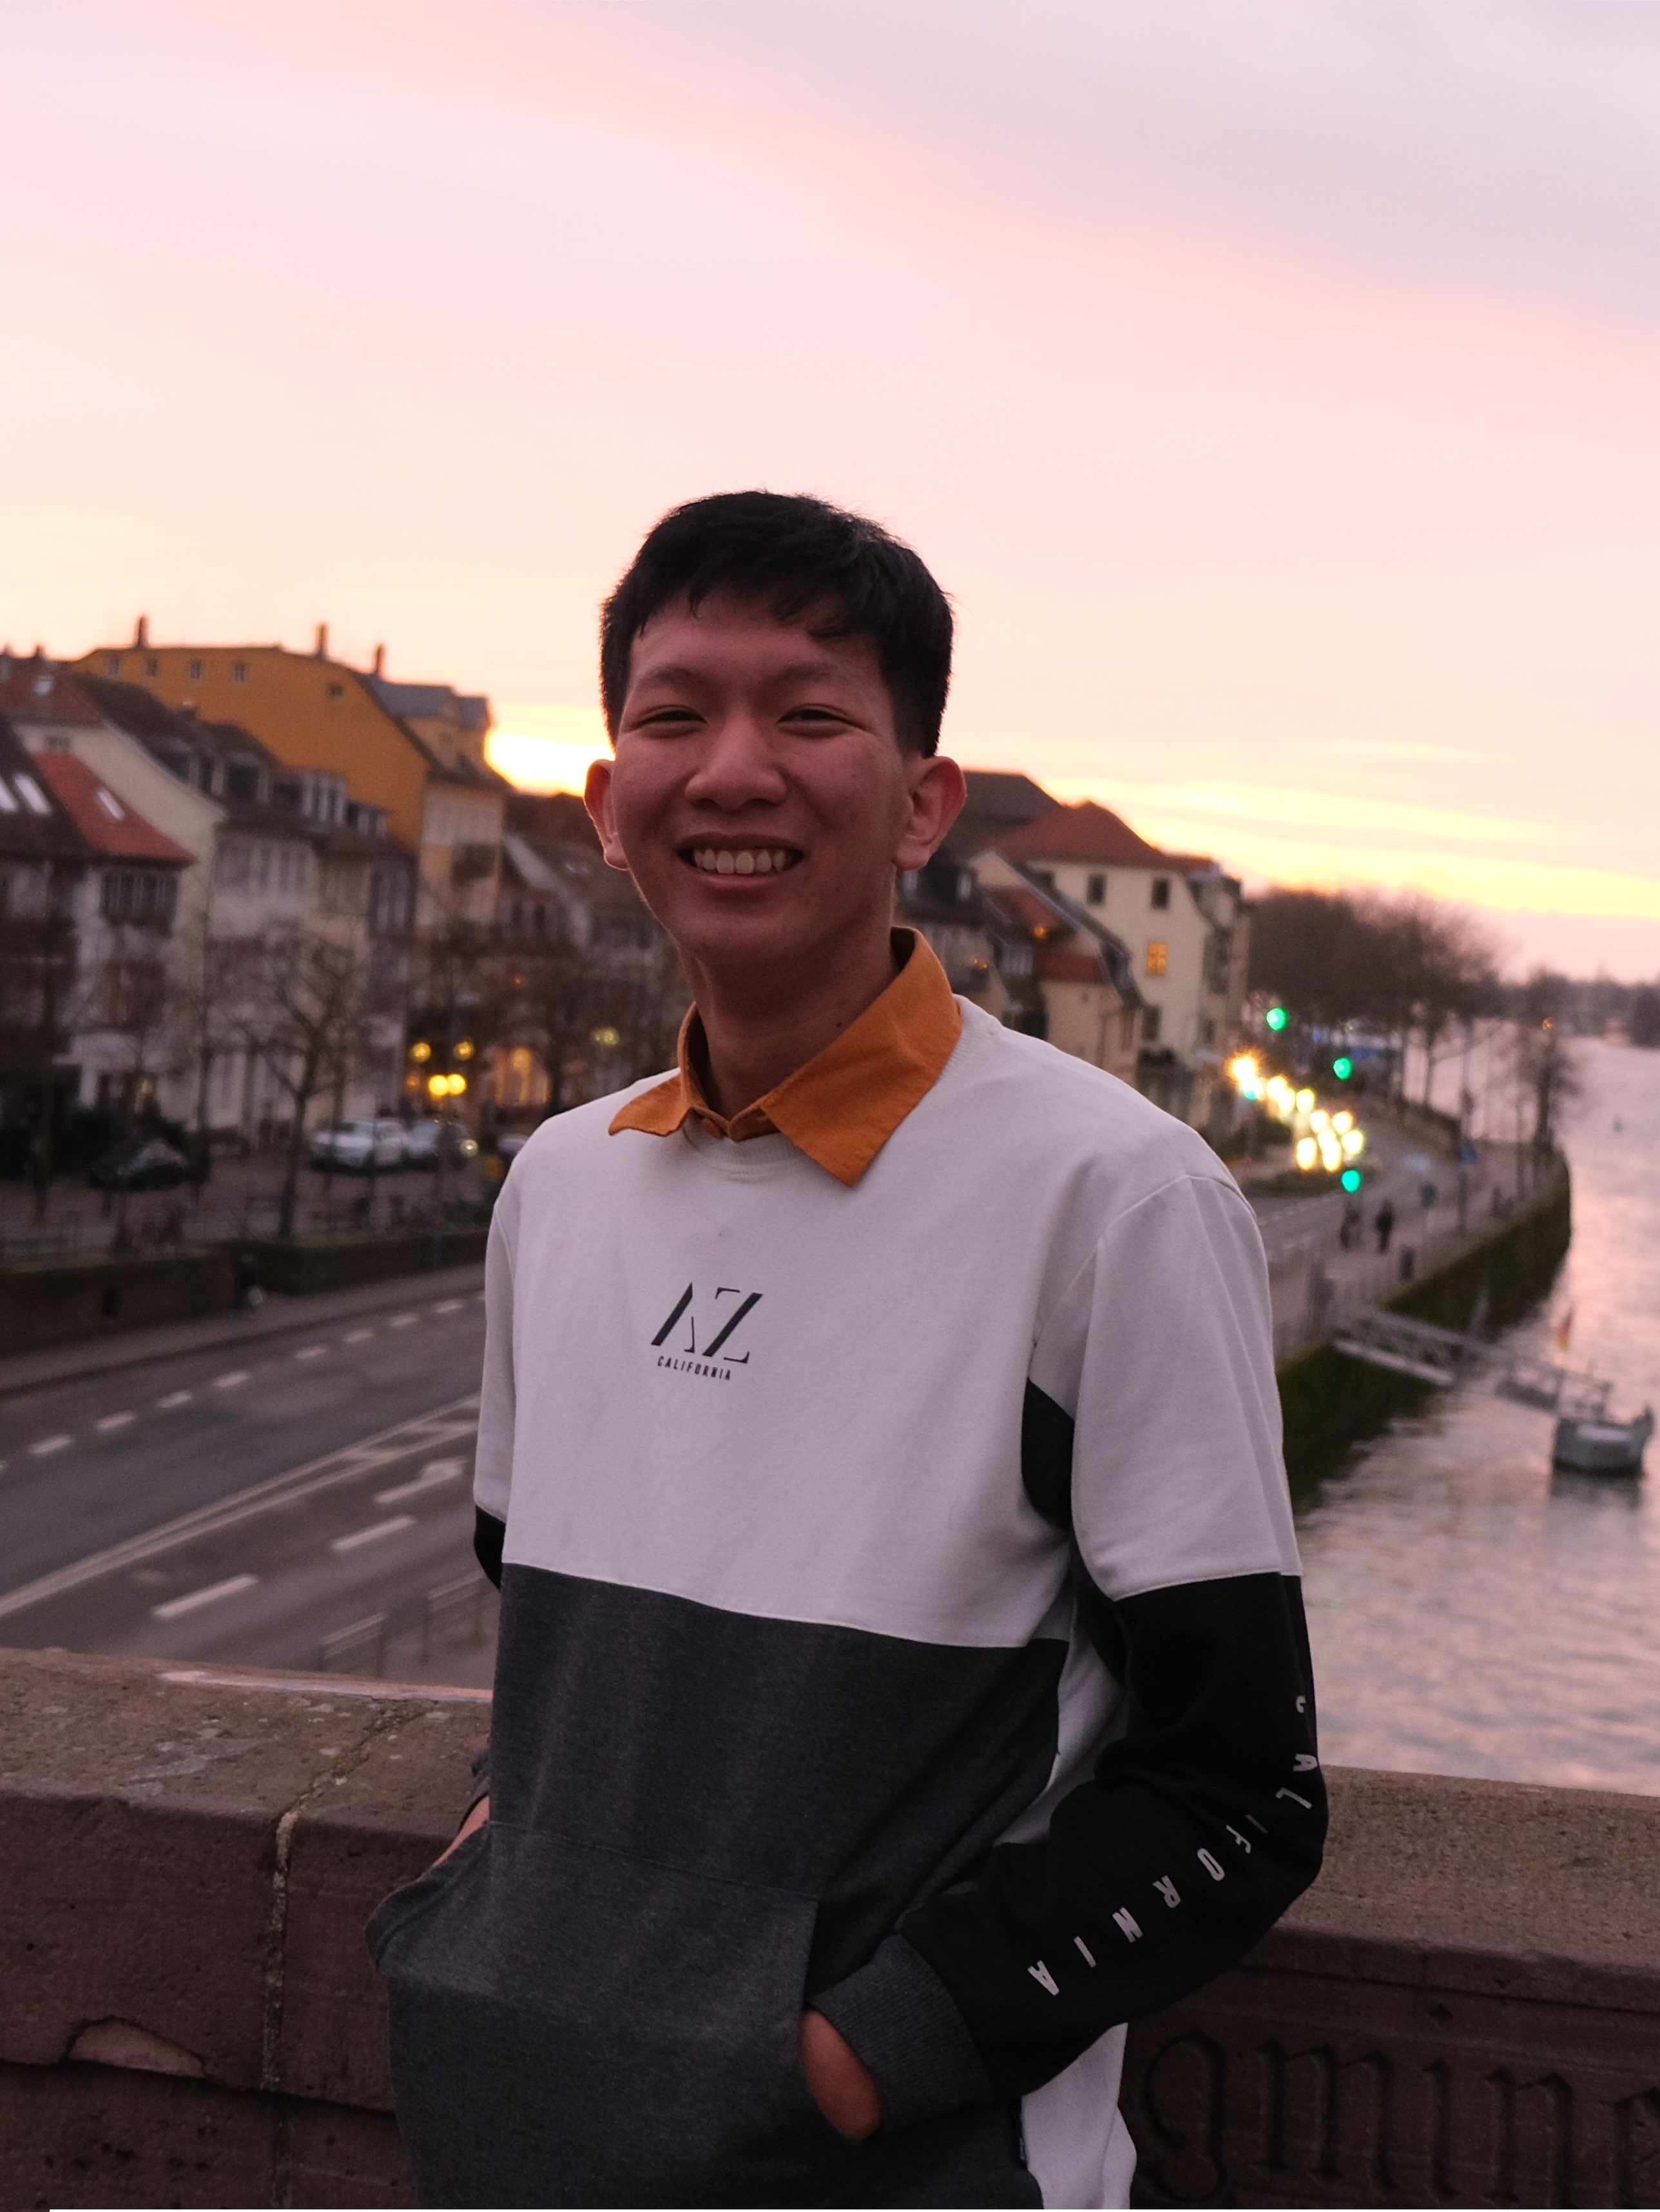
\includegraphics[height=0.2\textheight]{./ubah/Foto}
	\end{center}
%*********************************
\section*{Identitas Diri}
\begin{tabular}{p{3cm}cp{9cm}}
	%Masukan Identitas Disini.............
	Nama  		  & :&
		Lukas Purba Wisesa \\
	Tempat Lahir  & :&
		Rembang\\
	Tanggal Lahir &:& 
		24 November 1999\\
	Alamat        &:& J
		Jalan Diponegoro 28\\
%	Identitas 1   &:&
%		 Isi Identitas 1\\
%	Identitas 2   &:& 
%		Isi Identitas 2\\
%	Identitas 3   &:&
%		 Isi Identitas 3\\
%	Identitas 4   &:&
%		 Isi Identitas 4\\
\end{tabular}

\section*{Riwayat Pendidikan}
\begin{tabular}{p{3cm}cp{9cm}}
	2020-sekarang  & :&
		Program Master (S2), Departemen Teknik  Elektro, Fakultas Teknologi Elektro dan Informatika Cerdas, Institut Teknologi  Sepuluh Nopember\\
	&&\\
	2017-2021  & :&
		Program Sarjana (S1), Departemen Teknik  Elektro, Fakultas Teknologi Elektro dan Informatika Cerdas, Institut Teknologi  Sepuluh Nopember\\
	% &&\\
	% 0000-0000  & :&
	% 	Pendidikan 1\\
	% &&\\
	% 0000-0000  & :&
	% 	Pendidikan 2\\
	% &&\\
	% 0000-0000  & :&
	% 	Pendidikan 3\\
\end{tabular}


% \section*{Daftar Publikasi}

% \begin{enumerate}
% 	\item Setiyoutami, A., Anggraeni, W., Purwitasari, D., Yuniarno, E.M., Purnomo, M.H.,\textit{Extracting Temporal-Based Spatial Features in Imbalanced Data for Predicting Dengue Virus Transmission},
% 	Advances in Intelligent Systems and Computing, 2021, 1158, pp. 731–742
% 	\item Salsabila, F.N., Yuhana, U.L., Yuniarno, E.M., Purnomo, M.H., \textit{Sifte-math, a sifteo based mathematics assessment serious game for deaf children}, IES 2020 - International Electronics Symposium: The Role of Autonomous and Intelligent Systems for Human Life and Comfort, 2020, pp. 620–625, 9231578
	
	
% \end{enumerate}

% \section*{Riwayat Penelitian}
% \begin{enumerate}
% 	\item \lipsum[3]
% 	\item \lipsum[3]
% 	\item Penelitian Ke Tiga 
% 	\item Penelitian Ke Empat 
% \end{enumerate}
\section*{Tentang Penulis}
Lukas Purba Wisesa, merupakan seseorang mahasiswa yang 
berasal dari Institut Teknologi Sepuluh Nopember departemen Teknik Elektro. Penulis merupakan lulusan S1 Institut 
Teknologi Sepuluh Nopember. Dalam masa kuliah, penulis tertarik pada bidang pengembangan \textit{artificial 
intelligence}  dan pembelajaran mesin. Selain itu, penulis juga aktif dalam melakukan analisis sebagai hobi 
dimana pekerjaan penulis dapat diakses di github.com/lukaspurbaw. Penulis juga aktif dalam mengikuti kompetisi 
pengembangan model data science di ajang NDSC 2020. Bagi pembaca yang memiliki kritik, saran, atau pertanyaan 
mengenai laporan thesis ini dapat menghubungi penulis melalui surel lukaspurbaw@gmail.com.
\cleardoublepage}


\newcommand{\DaftarPustaka}{%\\renewcommand\bibname{Daftar Pustaka}
%\\addcontentsline{toc}{chapter}{\bibname}
%\\titlespacing*{\chapter}{0pt}{0ex}{5ex}
%\\appendix
%\%\bibliographystyle{apalike}
%\%\bibliographystyle{ieetr}
%\%\bibliographystyle{IEEEtranN}
%\\bibliographystyle{plainnat}
%\\bibliography{./ubah/pustaka}
%\\cleardoublepage
\renewcommand\bibname{Daftar Pustaka}
\addcontentsline{toc}{chapter}{\bibname}
\titlespacing*{\chapter}{0pt}{0ex}{5ex}
\appendix
%\bibliographystyle{IEEEtranN}
\bibliographystyle{IEEEtran}
\bibliography{IEEEabrv,./ubah/pustaka}
%\bibliography{library}
\cleardoublepage}

\tolerance=9999
\emergencystretch=10pt
\hyphenpenalty=10000
\exhyphenpenalty=100



%************************************
% 1. JENIS BUKU
%    Pilih Salah Satu 
%************************************
%     \ProposalDisertasi
%     \ProposalTesis 
     \Tesis{Magister Teknik (MT)}
%	\Disertasi{Doktor (Dr)}
%***************************

%\ProposalDisertasi
%\ProposalTesis 
%\Tesis{Magister Teknik (MT)}
%\Disertasi{Doktor (Dr)}


%*******************************
%2.  Tulislah Kode Yang Sesuai 
%*******************************
%\Kode{DISERTASI - EE186601}
\Kode{TESIS - EE184401}
%\Kode{Proposal Tesis}
%\Kode{Proposal Disertasi}
%*******************************

%*******************************
%  3. Judul Proposal, Tesis atau 
%     Disertasi 
%     dipilih Salah Satu 
%-------------------------------
% Tulislah Judul Dalam Bahasa Indonesia
\Judul{Deteksi Kerumunan untuk Pencegahan Penularan Virus Corona Berbasis Video Menggunakan Mask-RCNN}
% Tulislah Judul Dalam Bahasa Inggris
\JudulEng{Video-Based Crowd Detection for Preventing Corona Virus Transmission Using Mask-RCNN}
%************************************
% 4. Identitas Mahasiswa
% Format :\Mahasiswa{Nama}{Nrp}
%------------------------------------
\Mahasiswa{Lukas Purba Wisesa}{6022211057}
%************************************
% 5. Waktu Dan Ruang Ujian
%------------------------------------
%Tanggal Ujian 
\TanggalUjian{27 April 2022}
% Perioda wisuda  
\PeriodeWisuda{September 2022} 
%Hari ujian dan Tempat Ujian 
\HariUjian{Senin}
\TempatUjian{Ruang B204}


%************************************
%6. Identitas Pembimbing 
%   Maximal Tiga Pembimbing
%   Format : \PembimbingXXX{Nama}{Nip}
%-----------------------------------
%\scalebox{.95}[1.0]{xxx}
\PembimbingSatu{Reza Fuad Rachmadi, S.T., M.T., Ph.D}{198504032012121000}
\PembimbingDua{Dr. Eko Mulyanto Yuniarno, S.T., M.T.}{196806011995121009}
%\PembimbingTiga{Dr. Eko Mulyanto Yuniarno,ST. MT.}{132135221}

%************************************
% 7. Identitas Penguji 
%     Maximal 4 penguji
%     Format : \PengujiXXX{Nama}{Nip}
%-------------------------
\PengujiSatu{Dr. Adhi Dharma Wibawa, ST., MT.}{197605052008121003}
\PengujiDua{Eko Setijadi, ST., MT., Ph.D}{197210012003121002}
%************************************
% 8. Identitas Fakultas ------------------------------------
\Fakultas{Fakultas Teknologi Elektro Dan Informatika Cerdas}
\BeltFakultas{BeltFte}
%************************************
% 9. Identitas Departement
%-----------------------------------
\Departemen{Teknik Elektro}

\KaDep{Dedet Candra Riawan, ST., M.Eng., Ph.D}{197311192000031001}
%***********************************
% 10. Footer Identitas Program Studi 
%  Pada Cover
%----------------------------------
\CoverFooter{\normalsize
PROGRAM MAGISTER\\
	DEPARTEMEN TEKNIK ELEKTRO\\
	FAKULTAS TEKNOLOGI ELEKTRO DAN INFORMATIKA CERDAS\\
	INSTITUT TEKNOLOGI SEPULUH NOPEMBER\\
	SURABAYA\\
	2022}

%**********************************
%File Penting Yang Dapat di Edit:
%**********************************
%Abstrak :
%        ->\ubah\abstrak.tex
%Abstrak Bhs Inggris :
%        ->\ubah\abstrakEng.tex
%Kata Penggantar :
%        ->\ubah\pengantar.tex 
%Nomenklatur :
%        ->\ubah\Nomenklatur.tex
%Database Daftar Pustaka
%        ->\ubah\pustaka.bib
%DaftarRiwayatHidup 
%        ->\ubah\DaftarRiwayatHidup.tex
%----------------------------------
%**********************************
%Dokumen Utama
%----------------------------------
\begin{document}
%%%%%%%%%%%%%%%%%%%%%%%%%%%%%%%%%%%%%%%%%%%%
% FILE INI JANGAN DI UBAH ATAU MODIFIKASI
%%%%%%%%%%%%%%%%%%%%%%%%%%%%%%%%%%%%%%%%%%%%
\normalsize
\pagenumbering{roman}
\singlespacing
 \hyphenpenalty=1000
\tolerance=1000
\emergencystretch=2.5em
% Cover
%\addcontentsline{toc}{chapter}{Cover}
\begin{FontCover}
	\sffamily	
\thispagestyle{empty}
\begin{figure} [!t]
	
\includegraphics[keepaspectratio=true,scale=1,left]{lib/LogoITS.png}
	\caption*{}
	\label{fig:LogoITS}
\end{figure}
\vspace{1ex}
%\noindent\makebox[\linewidth]{\rule{\paperwidth}{10pt}}
\makebox[\linewidth]{\includegraphics[keepaspectratio=true,width=\paperwidth]{lib/\bbelt}}
\vspace{10ex}
\justify
\textbf{\Kodekk}
\vspace{1ex}
\justify
\Large
\begin{spacing}{1}
%Masukan Judul Tesis Disini
\flushleft
\textbf{\JdTesis}
\end{spacing}
\normalsize
\vfill
\justify

%\begin{spacing}{1}
\large
\MakeUppercase{\NamaMahasiswa}\\
NRP  \uppercase{\NrpMahasiswa}
\vspace{2ex}
\justify
\normalsize

\ifthenelse{\boolean{bMaster}}{\textbf{DOSEN PEMBIMBING}}{\textbf{PROMOTOR}}\\
\PbSatu\\
\ifthenelse{\boolean{PembimbingDua}}{\ifthenelse{\boolean{bMaster}}{}{\\\textbf{Co.PROMOTOR\\}}}{}
\ifthenelse{\boolean{PembimbingDua}}{\PbDua\\}{}
\ifthenelse{\boolean{PembimbingTiga}}{\PbTiga\\}{}
 
\vfill
\justify
\bdk
\vspace{1ex}
%\rmfamily
\normalfont
\end{FontCover}
\newpage
\cleardoublepage
% Lembar pengesahan
\addcontentsline{toc}{chapter}{LEMBAR PENGESAHAN}

\ifthenelse{\boolean{bThesis}}
{ \AddToShipoutPicture*{\BackgroundIm}
\begin{center}

\Large\textbf{\pPengesahan}
%\Large\textbf{PROPOSAL TESIS}
\end{center}
\begin{center}
\tsss\\
\textbf{\ggGelar}\\
di\\
\textbf{Institut Teknologi Sepuluh Nopember}\\
\vspace{1ex}
Oleh:\\
\textbf{\NamaMahasiswa}\\ 
\textbf{NRP:\NrpMahasiswa}\\ 
\vspace{1ex}
Tanggal Ujian :\TglUjian\\
Periode Wisuda : \PerWisuda\\
\vspace{1ex}
\end{center}
\begin{center}
Disetujui oleh:\\
\textbf{Pembimbing}:
\end{center}
\begin{enumerate}
\item \PbSatu \hfill ...............................\\
NIP:\NipPbSatu \vfill
\ifthenelse{\boolean{PembimbingDua}}{\item \PbDua\hfill ...............................\\
NIP:\NipPbDua}\vfill
\ifthenelse{\boolean{PembimbingTiga}}{\item \PbTiga \hfill ...............................\\
	NIP:\NipPbTiga}{}
\end{enumerate}	
\begin{center}
	\textbf{Penguji}:
\end{center}
\begin{enumerate}
	\item \PjSatu \hfill ...............................\\
	NIP:\NipPjSatu
	\vfill
	\item \PjDua \hfill ...............................\\
	NIP:\NipPjDua\vfill
\ifthenelse{\boolean{PengujiTiga}}{
	\item \PjTiga \hfill ...............................\\NIP:\NipPjTiga\vfill}{}
\ifthenelse{\boolean{PengujiEmpat}}{
	\item \PjEmpat \hfill ...............................\\ NIP:\NipPjEmpat\vfill}{}
\end{enumerate}	
\vfill
\begin{center}
	Kepala Departemen \Dep \\
	 \fak\\
	\vspace{9ex}
	\underline{\NmKaDep}\\
	Nip:\NipKaDep
\end{center}
\newpage
}
{
\begin{center}
\textbf{LEMBAR PENGESAHAN\\
	\prop}\\    
\end{center}
\vspace{5ex}
\begin{tabular}{p{2cm} c p{8cm}}
Judul&:&\JdTesis\\
Oleh &:&\NamaMahasiswa\\
Nrp&:&\NrpMahasiswa
\end{tabular}
\vspace{5ex}
\begin{center}
\textbf{Telah Diseminarkan  Pada}
\end{center}
\begin{tabular}{p{2cm} c p{8cm}}
Hari &:&\bHariUjian\\
Tanggal &:&\TglUjian\\
Tempat&:&\bTempatUjian
\end{tabular}
\vspace{5ex}
%\scalebox{.95}[1.0]{\PjSatu}

\begin{tabular}{p{8cm} p{8cm} }
\textbf{Penguji}& \textbf{Calon Pembimbing}\\
\vspace{8ex}\hspace{-10ex}1. \PjSatu&
\vspace{8ex}\hspace{-8ex}1. \PbSatu \\
\hspace{-7ex}Nip :\NipPjSatu&
\hspace{-5ex}Nip :\NipPbSatu\\
\vspace{8ex}\hspace{-10ex}2. \PjDua&
\ifthenelse{\boolean{PembimbingDua}}
{\vspace{8ex}\hspace{-8ex}2. \PbDua}{} \\
\hspace{-7ex}Nip :\NipPjDua&
\ifthenelse{\boolean{PembimbingDua}}
{\hspace{-5ex}Nip :\NipPbDua}{}\\
\ifthenelse{\boolean{PengujiTiga}}
{\vspace{8ex}\hspace{-10ex}3. \PjTiga}{}&
\ifthenelse{\boolean{PembimbingTiga}}
{\vspace{8ex}\hspace{-8ex}3. \PbTiga}{} \\
\ifthenelse{\boolean{PengujiTiga}}
{\hspace{-7ex}Nip :\NipPjTiga}{}&
\ifthenelse{\boolean{PembimbingTiga}}
{\hspace{-5ex}Nip :\NipPbTiga}{}\\


\ifthenelse{\boolean{PengujiEmpat}}
{\vspace{8ex}\hspace{-10ex}4. \PjTiga}{}& \\
\ifthenelse{\boolean{PengujiEmpat}}
{\hspace{-7ex}Nip :\NipPjEmpat}{}&\\
\end{tabular}
\newpage
}
\cleardoublepage

\ifthenelse{\boolean{bThesis}}
{
	\ifthenelse{\boolean{bMaster}}
	{
\chapter*{PERNYATAAN KEASLIAN TESIS}
\addcontentsline{toc}{chapter}{PERNYATAAN KEASLIAN TESIS}


\begin{spacing}{1.5}
	
	Dengan ini saya menyatakan bahwa isi keseluruhan Tesis saya dengan judul \textbf{\JdTesis} adalah benar-benar hasil karya intelektual mandiri, diselesaikan tanpa menggunakan bahan-bahan yang tidak diijinkan dan bukan merupakan karya pihak lain yang saya akui sebagai karya sendiri.
	
	Semua referensi yang dikutip maupun dirujuk telah ditulis secara lengkap pada daftar pustaka. Apabila ternyata pernyataan ini tidak benar, saya bersedia menerima sanksi sesuai peraturan yang berlaku.
	
	\hspace{30ex}Surabaya \today
	
	\vspace{10ex}
	
	\hspace{35ex}\underline{\NamaMahasiswa}
	
	\hspace{35ex}Nrp :\NrpMahasiswa
	
\end{spacing}
\cleardoublepage

}
{
	
	\chapter*{PERNYATAAN KEASLIAN DISERTASI}
	\addcontentsline{toc}{chapter}{PERNYATAAN KEASLIAN DISERTASI}
	
	\begin{spacing}{1.5}
		
		Dengan ini saya menyatakan bahwa isi keseluruhan Disertasi  saya dengan judul \textbf{\JdTesis} adalah benar-benar hasil karya intelektual mandiri, diselesaikan tanpa menggunakan bahan-bahan yang tidak diijinkan dan bukan merupakan karya pihak lain yang saya akui sebagai karya sendiri.
	
	Semua referensi yang dikutip maupun dirujuk telah ditulis secara lengkap pada daftar pustaka. Apabila ternyata pernyataan ini tidak benar, saya bersedia menerima sanksi sesuai peraturan yang berlaku.
	
	\hspace{30ex}Surabaya \today
	
	\vspace{10ex}
	
	\hspace{35ex}\underline{\NamaMahasiswa}
	
	\hspace{35ex}Nrp :\NrpMahasiswa
	
\end{spacing}
\cleardoublepage
}
}{}




% Kata pengantar
\newpage

\addcontentsline{toc}{chapter}{KATA PENGANTAR}
\begin{center}
\Large\textbf{Kata Pengantar}
\end{center}
\vspace{2ex}
%Tulis kata pengantar di sini
Puji syukur kehadirat Tuhan YME. atas segala limpahan berkat dan rahmat-Nya, penulis dapat menyelesaikan penelitian ini dengan judul \textbf{Deteksi Kerumunan untuk Pencegahan Penularan Virus Corona Berbasis Video Menggunakan Mask-RCNN}.

Penelitan ini disusun dalam rangka pemenuhan bidang riset di Departemen Teknik Elektro, serta digunakan sebagai persyaratan menyelesaikan pendidikan S2. Penelitian ini dapat terselesaikan tidak lepas dari bantuan berbagai pihak. Oleh karena itu, penulis mengucapkan terima kasih kepada:

\begin{enumerate}[nolistsep]
	\item Keluarga, Ibu, Bapak, dan kakak tercinta yang telah memberikan dorongan spiritual dan material dalam penyelesaian penelitian ini.
	\item Bapak Dedet Candra Riawan, ST., M.Eng., Ph.D. selaku Kepala Departemen Teknik Elektro, Fakultas Teknologi Elektro dan Informatika Cerdas (FTEIC), Institut Teknologi Sepuluh Nopoember.
	\item Bapak Reza Fuad Rachmadi, ST., MT., Ph. D selaku dosen pembimbing I yang telah memberikan arahan dan saran selama mengerjakan penelitian tugas akhir ini.
	\item Bapak Dr. Eko Mulyanto Yuniarno, ST., MT. selaku dosen pembimbing II yang telah memberikan arahan dan saran selama mengerjakan penelitian tugas akhir ini.
	\item Bapak Dr. Adhi Dharma Wibawa, ST., MT. dan Bapak Eko Setijadi ST, MT, Ph.D. selaku dosen penguji yang telah memberikan saran dan masukkan yang berguna untuk penulisan penelitian.
	\item Bapak-ibu dosen pengajar Departemen Teknik Elektro atas pengajaran, bimbingan, serta perhatian yang diberikan kepada penulis selama ini.
	\item Seluruh teman - teman dari Telematika 2020, Teknik Elektro yang telah mendukung dan menjadi teman seperjuangan saya.
  
\end{enumerate}

\vspace{26pt}
	\begin{flushright}
		\begin{tabular}[b]{c}
			Surabaya, April 2022
			\\
			\\
			\\
			Penulis
		\end{tabular}
	\end{flushright}

\cleardoublepage
\newpage
% Abstrak
\begin{spacing}{1}
\begin{center}
		\large\textbf{\JdTesis}
	\end{center}
	\normalsize
	\begin{adjustwidth}{-0.2cm}{}
		\ifthenelse{\boolean{bMaster}}{
		
		\begin{tabular}{lcp{0.9\linewidth}}
		Nama Mahasiswa &:& \NamaMahasiswa\\
			NRP &:&\NrpMahasiswa\\
			Pembimbing &:& 1. \PbSatu\\
			\ifthenelse{\boolean{PembimbingDua}}{& & 2. \PbDua\\}{}
			
			\ifthenelse{\boolean{PembimbingTiga}}{& & 3. \PbTiga\\}{}
			
			
			
		\end{tabular}
	}{
	\begin{tabular}{lcp{0.7\linewidth}}
		Nama Mahasiswa &:& \NamaMahasiswa\\
		NRP &:&\NrpMahasiswa\\
		Promotor &:&  \PbSatu\\
		\ifthenelse{\boolean{PembimbingTiga}}{
		\ifthenelse{\boolean{PembimbingDua}}{Co. Promotor&: & 1. \PbDua\\}{}
		\ifthenelse{\boolean{PembimbingTiga}}{& & 2. \PbTiga\\}{}
	}
{
	\ifthenelse{\boolean{PembimbingDua}}{\hspace{5ex}Co. Promotor&: & \PbDua\\}{}
	
}
	\end{tabular}

}

	
	\end{adjustwidth}
	\vspace{2ex}
	\begin{center}
		\Large\textbf{ABSTRAK}
	\end{center}
	\vspace{1ex}	
%Tulis Abstrak disini
Pandemi Covid-19 yang berlangsung dari tahun 2020 telah berlangsung selama 2 tahun. Walaupun
banyak masyarakat telah menerima vaksin, pemerintah tetap menegaskan masyarakat untuk melakukan protokol kesehatan
terutama di tempat umum.
Mengikuti saran dari WHO, salah satu protokol kesehatan yang perlu diterapkan adalah menjaga jarak satu sama lain
dengan jarak satu meter.
Namun, dalam penerapan protokol kesehatan, tentunya banyak masyarakat yang lalai untuk menerapkan hal tersebut.
Oleh karena itu, sebuah sistem deteksi yang dapat membantu memudahkan penerapan protokol kesehatan dirasa dibutuhkan.

Penelitian ini memanfaatkan algoritma Mask-RCNN yang digunakan untuk mendeteksi apakah terdapat kerumunan dalam suatu gambar yang diambil.
Objek yang dideteksi pada penelitian ini dibagi menjadi tiga kelas yaitu : Crowd, Group, dan Person. Kelas Crowd merupakan
kelas dimana terletak 4 orang atau lebih dalam radius 1 m, kelas group merupakan kelas dimana terdapat 2-3 orang dalam radius
1 m sedangkan kelas person merupakan kelas dimana hanya terdapat 1 orang dalam radius 1 m.
Mask R-CNN mendeteksi objek dengan cara memberikan beberapa proposal objek yang kemudian diproses dengan layer konvolusi dan \emph{fully connected layer}.
Keluaran dari layer konvolusi adalah \emph{mask} yang menunjukkan segmentasi gambar, sedangkan keluaran dari \emph{fully connected layers} adalah memberikan \emph{bounding box} serta menentukan nama kelas dari objek tersebut.
Hasil dari penelitian ini adalah model yang dapat mendeteksi adanya kerumunan dengan akurasi sebesar 88.79\%.

%Tulis Kata Kunci disini
\vspace{2ex}
\textbf{Kata kunci }: Mask R-CNN, Deteksi Kerumunan, \emph{deep learning}, Covid-19.
	
\end{spacing}
\cleardoublepage
\ifthenelse{\boolean{JudulTesisEng}}
{
	\begin{spacing}{1}
\begin{center}
		\large\textbf{\JdTesisEng}
	\end{center}
	\normalsize
	\begin{adjustwidth}{-0.2cm}{}
		\begin{tabular}{lcp{0.9\linewidth}}
		By &:& \NamaMahasiswa\\
			Student Identity Number &:&\NrpMahasiswa\\
			Supervisor &:& 1. \PbSatu\\
			\ifthenelse{\boolean{PembimbingDua}}{& & 2. \PbDua\\}{}
			\ifthenelse{\boolean{PembimbingTiga}}{& & 3. \PbTiga\\}{}
		\end{tabular}
	\end{adjustwidth}
	\vspace{2ex}
	
	\begin{center}
		\Large\textbf{ABSTRACT}
	\end{center}
	\vspace{1ex}	
%Tulis Abstrak disini
\textit{
  The Covid-19 pandemic that started in 2020 has been going on for 2 years. Although many people have received the vaccine, the government continues to emphasize the public to carry out health protocols especially in public places. Following the advice of WHO, one of the health protocols that need to be implemented is to keep a meter distance from each other. However, in implementing the health protocol, of course, many people tend to neglect the physical distancing practice. Therefore, a detection system that can help facilitate the implementation of health protocols especially physical distancing is needed. Crowd class is a class where there are 4 or more people within a 1 m radius, group class is a class where there are 2-3 people within a radius a meter while the person class is a class where there is only 1 person within a meter radius. This study utilizes the Mask-RCNN algorithm which is used to detect whether there is a crowd in an image taken. The objects detected in this study were divided into three classes, namely: Crowd, Group, and Person. The mask R-CNN algorithm detects objects by providing several object proposals which are then processed with the convolution layer and \emph{fully connected layer}. The output of the convolution layer is \emph{mask} which shows the image segmentation, while the output of \emph{fully connected layers} is to give the \emph{bounding box} and specify the class name of the object. The result of this study is a model that can detect crowds with an accuracy of 88.79\%
}

%Tulis Kata Kunci disini
\vspace{2ex}
\textbf{Keyword}: \emph{Mask R-CNN}, \emph{Crowd Detection}, \emph{Deep Learning}, \emph{Covid-19}.
\end{spacing}
}{}
\cleardoublepage

% Daftar isi
\renewcommand*\contentsname{DAFTAR ISI}
\titlespacing*{\chapter}{0pt}{0ex}{0ex}
\tableofcontents
\cleardoublepage
% Daftar gambar
\renewcommand*\listfigurename{DAFTAR GAMBAR}
\addcontentsline{toc}{chapter}{\listfigurename}
\titlespacing*{\chapter}{0pt}{0ex}{0ex}
\listoffigures
\cleardoublepage
% Daftar tabel
\renewcommand*\listtablename{DAFTAR TABEL}
\addcontentsline{toc}{chapter}{\listtablename}
\titlespacing*{\chapter}{0pt}{0ex}{0ex}
\listoftables
\cleardoublepage
% Nomenklatur
\addcontentsline{toc}{chapter}{NOMENKLATUR} % kata pengantar


\cleardoublepage

% Bab isi buku
\titleformat{\chapter}[display]{\bfseries\Large}{BAB \centering\thechapter}{0ex}{\vspace{0ex}\centering}[\vspace{0ex}]
\titleformat{\section}{\bfseries\large}{\MakeUppercase{\thesection}}{1ex}{}
\titleformat{\subsection}{\bfseries\large}{\MakeUppercase{\thesubsection}}{1ex}{}
\titleformat{\subsubsection}{\bfseries\large}{\MakeUppercase{\thesubsubsection}}{1ex}{}
\titlespacing*{\chapter}{0pt}{-4ex}{0pt}
\titlespacing{\section}{0pt}{0pt}{0pt}
\titlespacing{\subsection}{0pt}{0pt}{0pt}
\titlespacing{\subsubsection}{0pt}{0pt}{0pt}
% Indent paragraph
\setlength{\parindent}{0.8cm}
\begin{spacing}{1.5}
	
\begin{spacing}{1.2}
  \chapter{PENDAHULUAN}
\end{spacing}

\pagenumbering{arabic}
\vspace{4ex}

Penelitian ini memiliki beberapa latar belakang yang disebabkan oleh berbagai kondisi yang menjadi 
acuan. Selain itu juga terdapat beberapa permasalahan yang akan dijawab sebagai keluaran dari 
penelitian.

\section{Latar Belakang}
Virus Corona merupakan varian virus yang dapat menginfeksi manusia, gejala yang ditimbulkan oleh varian
virus ini meliputi infeksi paru-paru, pneumonia, demam, dan kesusahan bernapas. Dalam 2 dekade terakhir,
Virus Corona telah menyebabkan 3 pandemi besar \cite{10.1093/ajcp/aqaa029}.
Pada tahun 2002, sebuah varian virus corona yang dinamakan \textit{Severe Acute Respiratory Syndrome Corona Virus
(SARS-CoV)} menginfeksi manusia untuk pertama kalinya di Cina \cite{pmid12690091,pmid12690092},
varian virus ini menginfeksi 8.000 orang dan menyebabkan kematian bagi 750 orang. 10 Tahun kemudian pada tahun 2012,
varian baru virus corona yang dinamakan \textit{Middle East Repiratory Syndrome Corona Virus (MERS-CoV)} \cite{pmid23075143}.
MERS-COV menginfeksi 2.494 pasien dari beberapa negara di Timur Tengah dan menimbulkan korban jiwa sebanyak 866 orang. Kemudian varian Virus Corona
yang dinilai paling mematikan muncul pada pada Desember 2019 dan menyebabkan pandemi besar di Kota Wuhan, Provinsi Hubei,
Cina. Virus ini dinamakan SARS-CoV-2.

Penyakit yang ditimbulkan oleh SARS-CoV 2 dinamakan \textit{Corona Virus disease 2019} atau COVID-19,
gejala COVID-19 meliputi sakit kepala berat, demam, batuk, dan diare \cite{pmid32835023}.
Pada 29 Oktober 2021, COVID-19 telah menginfeksi lebih dari 450 juta orang dan mengakibatkan kurang lebih 6.000.000 korban jiwa
\cite{WHO}. Walaupun tingkat persentase kematian SARS-CoV 2 lebih rendah dibandingkan SARS-CoV maupun MERS-CoV,
kemampuan penyebaran SARS-CoV 2 lebih tinggi dibandingkan varian virus sebelum-sebelumnya \cite{pmid32226295}.
Virus SARS-CoV 2 dapat dengan mudah menyebar melalui \textit{droplet} atau tetesan air yang dikeluarkan dari
penderita. Penularan virus SARS-COV 2 sering terjadi kepada orang dengan kondisi sehat
saat penderita berbicara tanpa menggunakan masker kepada orang tersebut \cite{pmid32355904}.

Tidak hanya kerugian dalam dampak kesehatan, pandemi Covid-19 juga memberikan dampak ekonomi secara negatif dimana
bisnis pada berbagai sektor mengalami penurunan keuntungan \cite{pmid34337569}.
Sepanjang pandemi Covid-19, negara di seluruh dunia pun mengalami penurunan
pemasukan.  Rata-rata penurunan pemasukan tersebut bernilai 4.8\% pada negara dengan pemasukan kecil dan penurunan rata-rata
8.9\% pada negara dengan pemasukan besar. Salah satu contoh sektor yang mengalami kerugian besar ialah sektor aviasi. Penerbangan sektor internasional
menjadi terhambat dikarenakan negara-negara yang melakukan \textit{lockdown} dan menerapkan kebijakan
\textit{travel restriction}. Hal ini dibuktikan dengan penerbangan komersial Internasional Amerika
yang awalnya 4.000 penerbangan per bulan pada tahun 2019 turun menjadi 1.500 penerbangan per
bulannya pada tahun 2020 \cite{TRUONG2021102126}.

Mudahnya penularan virus SARS-CoV 2 serta besarnya efek negatif yang ditimbulkan menjadi alasan bagi pemerintah untuk
melakukan pencegahan dan mengurangi penularan virus SARS-CoV 2. \textit{World Health Organization}
menyarankan agar masyarakat menjaga jarak dan melakukan \textit{physical distancing}
dengan jarak satu meter \cite{WHO2}. Berdasarkan hal tersebut, Indonesia melakukan berbagai
kebijakan, beberapa diantaranya ialah pengadaan PPKM yang diatur pada PerPres no 21 tahun 2020 yang meliputi
peliburan sekolah dan tempat kerja, pembatasan kegiatan keagamaan, dan pembatasan kegiatan di tempat umum.
Selain kebijakan tersebut Kepala Kepolisian Negara Republik Indonesia juga mengeluarkan maklumat
yang melarang adanya aktivitas berkumpulnya massa dalam jumlah banyak, baik di tempat umum maupun di lingkungan
sendiri \cite{DJALANTE2020100091}.

Dalam melakukan pengawasan kerumunan dan mengurangi penularan virus corona, sering kali petugas
melakukan patroli dan peninjauan lokasi secara langsung. Namun patroli tentunya membutuhkan personil untuk datang ke 
lokasi dan hanya dilakukan pada jam serta hari-hari tertentu. Tidak hanya itu, patroli yang dilakukan tidak dapat
mendata tempat keramaian secara detail untuk analisa lebih lanjut. Dengan permasalahan tersebut,
penulis menawarkan solusi untuk melakukan pengawasan kerumunan dengan pembelajaran mesin menggunakan
algoritma mask R-CNN. Selain untuk pengawasan kerumunan untuk mengurangi penyebaran Covid-19, data
deteksi kerumunan ini juga dapat digunakan untuk desain arsitektur tempat umum seperti ruang tunggu,
maupun pintu masuk ruangan yang lebih mendukung gaya hidup pasca Covid-19.

\section{Rumusan Masalah}
Pemantauan kerumunan selama ini masih dijalankan secara pemeriksaan manual. Petugas masih harus melakukan
pemantauan pada video cctv atau datang ke lokasi langsung untuk melakukan patroli. Jika kondisi wilayah yang
perlu diamati bertambah dan sumber daya manusia pemerintah kota tidak mencukupi dalam melaksanakan pemantauan kerumunan di
berbagai wilayah, maka kerumunan tidak dapat diketahui dan berpotensi besar menjadi salah satu media penyebaran
Virus Corona. Berdasarkan penjelasan di atas, maka akan dikembangkan sebuah sistem deteksi kerumunan otomatis
menggunakan algoritma kecerdasan buatan Mask R-CNN. Harapannya tidak hanya data deteksi kerumunan yang diberikan
dapat digunakan untuk mengatasi dan melaporkan situasi kerumunan,
data ini juga dapat digunakan dalam pemodelan penularan virus maupun desain ruang yang lebih baik.

\section{Tujuan}
Tujuan utama dari penelitian ini adalah mempersiapkan teknologi untuk melakukan
pengamatan secara otomatis terhadap suatu wilayah dalam rangka mengurangi penyebaran virus
corona maupun mengambil informasi mengenai kerumunan di beberapa wilayah,
serta mengurangi sumber daya manusia yang diperlukan untuk melakukan pengawasan kerumunan.
Selain untuk mempersiapkan teknologi masa depan yang dapat memonitoring kerumunan, 
deteksi kerumunan secara otomatis juga dapat digunakan untuk melihat apakah PPKM yang 
dilaksanakan berhasil atau tidak dengan mengetahui jumlah kerumunan yang terjadi. 
Semua hal ini dilakukan dalam rangka menurunkan kasus Covid-19 dan mengurangi penyebaran Virus Corona.

\section{Batasan Masalah}

Untuk memfokuskan permasalahan yang diangkat, maka dilakukan pembatasan masalah.
Batasan - batasan masalah tersebut diantaranya adalah :

\begin{enumerate}[itemsep=-0.2em]
      \item Data yang diambil merupakan data video dengan kondisi nyata di salah satu pusat
            perbelanjaan Surabaya, Jawa Timur, Indonesia.
      \item Algoritma yang digunakan dalam penelitian ini ialah Mask R-CNN.
      \item Pengambilan data dilakukan dari ketinggian dan sudut pengambilan yang akan didefinisikan pada Bab 3.
      \item Kelas yang dideteksi dibedakan menjadi tiga kelas yaitu \textit{person, group, crowd} yang didefinisikan oleh peneliti.
      \item Pengambilan data dilakukan pada bulan Januari 20222 di Pasar Atom Surabaya pada jam 1 siang hingga 4 sore.
      \item Objek yang dideteksi merupakan objek orang segala usia.
      \item Hasil keluaran dari penelitian ini adalah model pembelajaran mesin yang dapat digunakan untuk mendeteksi kerumunan Indonesia.

\end{enumerate}

\section{Manfaat}
Diharapkan penelitian ini dapat mendeteksi kerumunan dalam rangka membantu penanganan Covid-19 
maupun pandemi masa depan yang mungkin terjadi. Hasil dari deteksi kerumunan dapat digunakan sebagai
sistem \textit{monitoring} atau sebagai penghasil data mengenai perilaku masyarakat pasca pandemi Covid-19,
selain itu, diharapkan penelitian ini dapat membantu penanganan pandemi di masa depan.

\section{Sistematika Penulisan}

Laporan penelitian ini tersusun dalam sistematika dan terstruktur sehingga mudah
dipahami dan dipelajari oleh pembaca maupun seseorang yang ingin melanjutkan penelitian ini.
Alur sistematika penulisan laporan penelitian ini yaitu :

\begin{enumerate}[topsep=0em]

      \item \textbf{BAB I Pendahuluan}
            Bab ini berisi uraian tentang latar belakang permasalahan, penegasan
            dan alasan pemilihan judul, sistematika laporan, tujuan dan metodologi penelitian.
      \item \textbf{BAB II Tinjauan Pustaka}

            Bab ini berisi tentang uraian secara sistematis teori - teori yang
            berhubungan dengan permasalahan yang dibahas pada penelitian ini.
            Teori - teori ini digunakan sebagai dasar dalam penelitian, yaitu informasi terkait
            \textit{Deep Learning}, \textit{Object Detection},
            \textit{Mask R-CNN}, dan teori - teori penunjang lainnya.

      \item \textbf{BAB III Desain dan Implementasi Sistem}

            Bab ini berisi tentang penjelasan - penjelasan terkait eksperimen yang akan dilakukan,
            langkah - langkah pengambilan dataset dan proses pembagian kelas kerumunan.
            Untuk mendukung hal tersebut, maka ditampilkan pula \textit{workflow} agar proses penelitian
            yang akan dibuat dapat terlihat dan mudah dibaca untuk proses pembuatan pada pelaksanaan tugas akhir.

      \item \textbf{BAB IV Pengujian dan Analisa}

            Bab ini menjelaskan tentang hasil serta analisis yang didapatkan dari pengujian yang
            dilakukan mulai dari hasil pengujian \textit{precision}, \textit{recall}, \textit{Confusion Matrix}
            serta rekomendasi penggunaan model.

      \item \textbf{BAB V Penutup}

            Bab ini berisi penutup yang berisi kesimpulan yang diambil dari penelitian dan
            pengujian yang telah dilakukan. Saran mengenai langkah selanjutnya untuk pengembangan
            lebih lanjut juga dituliskan pada bagian ini.

\end{enumerate}
	\cleardoublepage
	\chapter{KAJIAN PUSTAKA}

\section*{ }
Demi mendukung penelitian ini, dibutuhkan beberapa teori penunjang sebagai bahan acuan dan referensi. 
Dengan demikian penelitian ini menjadi lebih terarah.
\vspace{1ex}

\section{Covid-19}

Covid-19 merupakan salah satu penyakit dengan daya penyebaran paling tinggi yang disebabkan oleh \textit{Severe
acute respiratory syndrome (SARS-CoV-2)}. Penyakit Covid-19 telah menyebabkan banyaknya korban jiwa serta kerugian
materi di berbagai aspek ekonomi. WHO menetapkan Covid-19 sebagai pandemi global pada tanggal 11 maret 2020. Pada
awalnya, dapat dikatakan bahwa pelayanan kesehatan tidak memiliki sistem yang baik dalam penanganan Covid-19.
Walaupun sistem pelayanan kesehatan terutama di rumah sakit dalam menangangi Covid-19 semakin lama semakin membaik
dan telah mengalami banyak kemajuan, beberapa mutasi yang mengubah karakteristik virus secara drastis dapat menimbulkan
semakin banyak korban jiwa maupun kerugian materi. Oleh karena itu pembatasan penyebaran virus dan variannya 
harus tetap dilakukan.

Hingga saat ini varian SARS-CoV-2 yang disebabkan oleh mutasi virus tetap terus diteliti, beberapa varian yang 
dianggap membahayakan karena meningkatnya daya penularan dan keagresifan virus diberi nama \textit{Variant 
of Concern (VOC)}.
Pada tanggal 11 Desember 2021, WHO menetapkan adanya lima \textit{variant of concern} yaitu :

\begin{enumerate}
    \item \textbf{Alpha (B.1.1.7)} 
    
    Varian Alpha merupakan \textit{variant of concern} pertama yang muncul di Inggris pada akhir Desember 2020 
    \cite{pmid33476315}. Varian ini memiliki 17 mutasi dan mempunyai peningkatan pada daya lekat ke sel 
    \textit{host} \cite{pmid33501442, pmid33658326}. Varian ini memiliki peningkatan transmisi 43\% Hingga
    82\% dibandingkan varian SARS-CoV-2 sebelumnya \cite{pmid33658326}. 

    \item \textbf{Beta (B.1.351)} 
    
    Varian Beta pertama kali dilaporkan di Afrika Selatan pada Desember 2020 dan menyebabkan adanya gelombang 
    kedua pandemi Covid-19 di Afrika Selatan \cite{pmid33690265}. Varian ini memiliki 9 mutasi \cite{pmid33630820}
    dimana varian ini memiliki kemampuan untuk menurunkan antibodi sehingga dapat menginfeksi orang yang telah
    divaksin atau menerima plasma konvalesen \cite{pmid33688656}.
    
    \item \textbf{Gamma(P.1)} 
    
    Varian Gamma pertama kali dilaporkan di Brazil pada awal Januari 2021 \cite{pmid33688664}. Varian Gamma
    memiliki 10 mutasi. Efek dari mutasi ini hampir mirip dengan varian Beta dimana varian ini memiliki kemampuan
    untuk menurun antibodi orang yang terinfeksi \cite{pmid33688656}.

    \item \textbf{Delta (B.1.617.2)}
    
    Varian Delta pertama kali dilaporkan di India pada Desember 2020. Varian ini merupakan salah satu yang paling
    berbahaya karena pasien yang terkena oleh varian delta mempunyai peluang kematian 133\% lebih tinggi dibandingkan
    varian awal dan 235\% lebih memungkinkan untuk masuk ke ruang ICU. Vaksin yang diberikan juga mengalami penurunan
    efektivitas melawan varian delta \cite{pmid34698149}.

    \item \textbf{Omicron (B.1.1.529)} 
    Varian Omicron pertama kali dilaporkan di Afrika Selatan pada November 2021 \cite{pmid34876769}. Varian 
    Omicron mempunyai 30 mutasi \cite{pmid34860154} dan 2,8 kali lebih menular dibandingkan varian delta. 

\end{enumerate}

\subsection{Cara Penularan}
Penyakit Covid-19 yang disebabkan oleh SARS-CoV-2 dapat menular melalui cara-cara berikut :

\begin{itemize}
    \item Transmisi SARS-CoV-2 yang paling umum ialah melalui paparan \textit{droplet} yang dikeluarkan oleh
    individu lain yang telah terinfeksi oleh virus tersebut.

    \item Melalui material seperti besi dan plastik yang terpapar oleh SARS-CoV-2, SARS-CoV-2 dapat bertahan 
    selama 72 jam pada material besi dan plastik, 24 jam pada material kardus, dan 4 jam pada material tembaga.
    Tingkat kontaminasi semakin meningkat jika barang tersebut digunakan oleh orang banyak contoh seperti tetikus
    komputer di rumah sakit \cite{pmid32275497}.

    \item Melalui transmisi vertikal dari ibu yang hamil kepada bayi yang akan dilahirkan, namun kasus ini jarang 
    terjadi, sebuah penelitian \cite{pmid32739398} mengungkapkan bahwa dari 936 bayi yang dilahirkan dari ibu yang positif Covid-19,
    hanya 27 bayi yang dinyatakan positif Covid-19.

\end{itemize}

\subsection{Epidemiologi}
Dari tulisan sebelumnya, sudah dapat diketahui bahwa Covid-19 dapat menimbulkan kematian, namun terdapat 
beberapa faktor yang mempengaruhi apakah pasien akan sembuh dari Covid-19 atau tidak. Beberapa faktor tersebut
adalah umur, gender, dan penyakit yang diderita oleh pasien. Pasien yang mempunyai umur di atas 65 tahun mempunyai
kemungkinan untuk meninggal lebih besar dibandingkan kelompok usia lain \cite{pmid33356661}. Penelitian lain
\cite{pmid32555134} mengakatakan bahwa pasien-pasien Covid-19 yang memiliki obesitas, penyakit jantung, penyakit
kronis ginjal, diabetes, penyakit kronis paru-paru, kanker, dan kebiasaan merokok lebih berpeluang untuk dirawat
di rumah sakit (45,4\%) dibandingkan yang tidak memiliki kondisi tersebut (7,6\%). Selain itu pasien-pasien
yang memiliki kondisi tersebut 12x lebih berpotensi untuk tidak sembuh dan meninggal (19,5\%) dibandingkan pasien
yang tidak memiliki kondisi kesehatan tersebut (1,6\%).

Kemudian jika dibedakan berdasarkan gender, berdasarkan data yang diperoleh, pasien pria lebih memiliki risiko
yang lebih tinggi untuk menjadi pasien Covid-19 dan meninggal akibat Covid-19 dibandingkan pasien perempuan 
\cite{pmid32450906}. Peneliti pun juga meniliti apakah ras dan etnik mempunyai hubungan dengan Covid-19. Hasil
dari meta-analisis peneliti Amerika dan Inggris mengatakan bahwa orang-orang dengan ras afrika, hispanik (keturunan eropa),
dan orang asia memiliki kecenderungan untuk mengalami Covid-19 \cite{pmid33200120}, dimana tingkat kematian 
tertinggi terjadi pada orang hispanik \cite{pmid33830988}.

\subsection{Dampak Covid-19}
Sangat banyak dampak negatif yang diberikan saat terjadinya pandemi Covid-19, jumlah korban jiwa karena kejadian
ini telah mencapai lebih dari 6 juta orang \cite{WHO}. Pandemi Covid-19 juga membawa dampak kemiskinan di berbagai
negara. Di awal pandemi Covid-19, masyarakat di beberapa negara melakukan \textit{panic buying} \cite{CHEN2022102970}.
Tindakan \textit{panic buying} ini terjadi karena ketakutan dari masyarakat untuk melakukan aktivitas di luar dan
kepanikan masyarakat dalam rangka bertahan hidup. Hal ini pun secara otomatis meningkatkan kelangkaan bahan makanan serta harga dari kebutuhan pokok sehari-hari.
Tingkat kemiskinan yang naik dan kelangkaan bahan makanan pun dapat dikatakan terjadi karena pandemi Covid-19 
\cite{HEADEY2022100626}. Tidak hanya kesehatan jasmani yang menjadi ancaman, beberapa penelitian juga membahas mengenai
dampak Covid-19 pada kesehatan mental masyarakat \cite{CAMPOARIAS2022114337}. Covid-19 memberikan dampak depresi
stress, dan trauma terutama pada masyarakat golongan bawah. Diskriminasi terhadpa pasien Covid-19 yang sembuh pun
turut mendukung kemungkinan terjadinya stress dan depresi pada orang yang sembuh dari penyakit Covid-19.

Dalam segi ekonomi, Covid-19 telah memberikan penurunan yang drastis pada pasar saham, performa industri, serta
menurunkan jumlah pembeli di pasar-pasar tradisional maupun modern. Pada pasar saham, penurunan indeks saham yang
terjadi pun berkolerasi erat dengan tingkat kasus Covid-19 yang terjadi \cite{UDEAJA2022e01076}. Penurunan nilai
saham ini pun dapat dikatakan terjadi berbagai belahan dunia. Performa yang menurun juga dialami oleh berbagai industri
mulai dari industri kreatif \cite{KHLYSTOVA20221192} hingga industri-industri besar \cite{XU202287}.

\subsection{Cara Penanggulangan}
Cara penanggulangan (termasuk cara pencegahan) Covid-19 dibedakan menjadi dua macam, yaitu dengan interfensi memprediksi
dan non-interfensi medis. Interfensi medis membahas mengenai penanganan Covid-19 yang meliputi penggunaan terapi medis,
obat-obatan, dan vaksinasi. Sedangkan non-interfensi medis membahasa mengenai regulasi maupun penyuluhan
bagi masyarakat.

\begin{itemize}
    \item \textbf{Penanganan Medis}
    
        Penanganan pandemi Covid-19 saat ini telah dilakukan dengan cara vaksinasi dan pemberian \textit{booster}
        pada masyarakat untuk meningkatkan daya tahan tubuh dan menurunkan efek negatif yang diberikan oleh virus
        SARS Cov-2 kepada tubuh penerima vaksin. Pemberian vaksin Covid-19 yang dilakukan secara umum telah memberikan efek melindungi 
        tubuh manusia serta memberikan kasiat klinis terhadap SARS-CoV 2 setidaknya 60\% bergantung pada jenis
        vaksin yang diberikan. Salah satu vaksin yang memberikan efek paling baik salah satunya adalah vaksin
        BNT162b2 yang lebih kita kenal sebagai vaksin pfizer mempunyai efektivitas 95\% terhadap penerima vaksin 
        kedua \cite{pmid33301246}.

        Penanganan Medis lainnya khususnya penanganan yang digunakan saat pasien terkena Covid-19 adalah terapi
        plasma konvalesen. Walaupun terapi ini diperbolehkan, terdapat beberapa penelitian yang memberikan data
        bahwa terapi plasma konvalesen tidak lebih baik dibandingkan dengan terapi pada umumnya \cite{pmid33232588,pmid32492084}.
        Pemberian antibodi juga dapat membantu pasien khususnya REGN-COV2 dan VIR-7831 sangat dianjurkan. antibodi
        REGN-COV2 menurunkan jumlah pasien yang meninggal hingga 70\% \cite{pmid33332778}, sedangkan antibodi 
        VIR-7831 menurunkan kemunungkinan pasien meninggal atau perlu dirawat di rumah sakit hingga 80\%. 

    \item \textbf{Penanganan Non Medis}
    
        Beberapa penanganan non medis pada pandemi Covid-19 juga telah dilaksanakan, beberapa hal penting yang dilakukan
        sebagai upaya penanganan non medis adalah penggunaan masker dan menjaga jarak satu sama lain. Penelitian \cite{HANTHANANARACHCHILAGE2021111458}
        mengatakan bahwa dengan menjaga jarak dan menggunakan masker, menurunkan persentasi prediksi terjadinya korban
        jiwa 25\% hingga 45\%. Penanganan ini merupakan hal yang termudah untuk dilakukan dalam menurunkan kasus
        Covid-19 yang terjadi. Penanganan non medis juga dapat dilakukan dengan cara menutup bandara, membatasi 
        kegiatan pariwisata, dan menutup beberapa tempat pusat kegiatan masyarakat \cite{GE2022102649}.

\end{itemize}

\section{Machine Learning}

\textit{Machine Learning} atau Pembelajaran Mesin adalah salah satu cabang dalam kecerdasan buatan dan ilmu 
komputer yang menggunakan data dan algoritma untuk meniru manusia dalam mempelajari sesuatu \cite{ibm_ml_expl}. 
Salah satu hal yang membuat pembelajaran mesin sangat diminati adalah kemampuannya untuk menyelesaikan suatu 
tugas dengan sedikit intervensi dari manusia.

Sekarang ini, pembelajaran mesin adalah salah satu fokus yang cukup diminati pada bidang \textit{data science}. 
Dimana dengan menggunakan pembelajaran mesin, diharapkan suatu kecerdasan buatan dapat menyelesaikan beberapa 
tugas yang bagi komputer cukup rumit seperti misalnya, memberikan prediksi yang akurat berdasarkan data, 
melakukan klasifikasi pada teks maupun pada gambar, melakukan pemrosesan citra guna mengenali objek di dalam 
citra tersebut, dan masih banyak lagi.

Untuk prosesnya sendiri, awalnya kita harus mengumpulkan data, data ini dapat kita ambil dari  berbagai sumber 
atau bisa juga menggunakan data yang berasal dari instansi atau pribadi (data yang kita buat sendiri). 
Selanjutnya adalah proses \textit{training} dimana data akan dimasukkan ke dalam model pembelajaran mesin 
yang sudah dipilih. Kita dapat merubah beberapa parameter dari model tersebut untuk meningkatkan akurasi dari 
suatu model pembelajaran mesin. Terakhir adalah melakukan proses \textit{testing}, dimana model akan melakukan 
prediksi pada set data yang berbeda dari yang digunakan pada saat proses \textit{training}. Apabila ternyata 
tingkat akurasi dirasa kurang memadai, dapat dilakukan proses \textit{re-training} sampai tingkat akurasi 
nya dirasa cukup. Hasil akhir dari proses ini adalah sebuah model pembelajaran mesin yang dapat digunakan 
walaupun menggunakan data yang berbeda \cite{mit_ml_expl}.

\subsection{\textit{Supervised Learning}}
Salah satu cabang dalam bidang pembelajaran mesin. Disini data yang dijadikan masukan ke model sudah diberikan 
label atau struktur tertentu \cite{ms_ml_expl}. Berdasarkan dari data berlabel tersebut, sebuah model akan 
merubah parameter internalnya agar mendekati atau sesuai dengan label yang diberikan \cite{ibm_ml_expl}. 
Salah satu contoh model pembelajaran mesin dengan metode pembelajaran seperti ini adalah \textit{Linear 
Regression, Random Forest}, dan sebagainya.

\subsection{\textit{Unsupervised Learning}}
Salah satu cabang dalam bidang pembelajaran mesin. Disini data yang dijadikan masukan ke model tidak diberikan 
label sama sekali. Nantinya model akan membuat pengelompokan (\textit{clusters}) dan hubungan berdasarkan dari 
data yang diberikan \cite{mit_ml_expl}. Contoh model yang menggunakan metode pembelajaran ini adalah 
\textit{K-NN clustering}.

\subsection{\textit{Reinforcement Learning}}
Salah satu cabang dalam bidang pembelajaran mesin. Disini model tidak diberikan data awal sama sekali, 
namun, model dibiarkan melakukan proses percobaan secara mandiri terus-menerus sampai tercapai hasil atau 
respon yang diinginkan. Apabila terdapat parameter yang menghasilkan respon positif, maka parameter tersebut 
disimpan dan digunakan sebagai masukan untuk iterasi \textit{training} berikutnya \cite{mit_ml_expl}.

\section{\textit{Deep Learning}}

Mirip seperti pembelajaran mesin, \textit{Deep Learning} juga merupakan salah satu bidang dalam bidang 
kecerdasan buatan. Yang membedakan antara pembelajaran mesin biasa dengan \textit{deep learning} adalah 
\textit{deep learning} mengacu pada penggunaan \textit{layer} dan \textit{artificial neural network} hingga
mempunyai \textit{multiple hidden layer}, sedangkan \textit{machine learning} lebih mengacu kepada seluruh 
algoritma yang dapat diterapkan untuk menemukan \textit{rules} dari serangkaian data. 
Keuntungan dari model jenis ini adalah model ini dapat memproses masukan yang paling 
abstrak sekalipun, sehingga menghilangkan proses ekstraksi fitur secara manual \cite{mathwork_deeplearning}. 
Namun, karena \textit{deep learning} memiliki \textit{layers} yang sangat banyak, maka diperlukan jumlah data 
yang jauh lebih banyak pula. Karena itu, sebuah model \textit{deep learning} memerlukan daya komputasi 
yang jauh lebih besar dibandingkan dengan model pembelajaran mesin biasa. Setiap \textit{layer} dapat 
memiliki fungsi dan tanggung jawabnya masing - masing \cite{mit_ml_expl}, seperti misal apabila kita 
menggunakan \textit{deep learning} untuk mendeteksi angka plat nomor di kendaraan bermotor, bisa saja beberapa 
layer pertama berfungsi untuk mendeteksi letak plat nomor dalam suatu citra, kemudian beberapa layer 
selanjutnya berfungsi untuk mengambil bentuk dari setiap objek dalam plat nomor tersebut, beberapa layer 
terakhir berfungsi untuk mengenali bentuk - bentuk dari objek menjadi tulisan teks. Semakin banyak layer yang 
digunakan, maka semakin tinggi pula kemungkinan kita melakukan sesuatu yang lebih kompleks \cite{mit_ml_expl}.

\section{Artificial Neural Network}
Dalam pengaplikasiannya \textit{Deep learning} menggunakan jaringan saraf neuron yang bekerja layaknya seperti
otak manusia. Jaringan neuron ini disebuat jaringan neuron buatan atau \textit{artificial neural network} (ANN).
ANN disusun oleh neuron buatan (\textit{artificial neuron}) yang dapat menerima input berupa suatu angka, memprosesnya, 
kemudian menyalurkan output dari proses yang terjadi. Proses yang dilakukan oleh setiap \textit{artificial neuron}
adalah mencari nilai \textit{weight} terbaik agar nilai tersebut dapat memberikan \textit{output} dengan error paling
kecil setelah diproses dengan sebuah \textit{activation function}. Nilai \textit{weight} pada sebuah
neuron buatan dapat berubah dan nilai perubahannya dipengaruhi \textit{learning rate}. \textit{Learning rate}
adalah sebuah paramater yang mengatur seberapa besar perubahan yang harus terjadi pada \textit{weight} suatu neuron
dalam mencapai nilai optimal dimana nilai optimal yang dimaksud ialah nilai \textit{weight} yang memberikan error terkecil
jika dibandingkan pada data awal.

\begin{figure}[h!]
    \begin{center}
      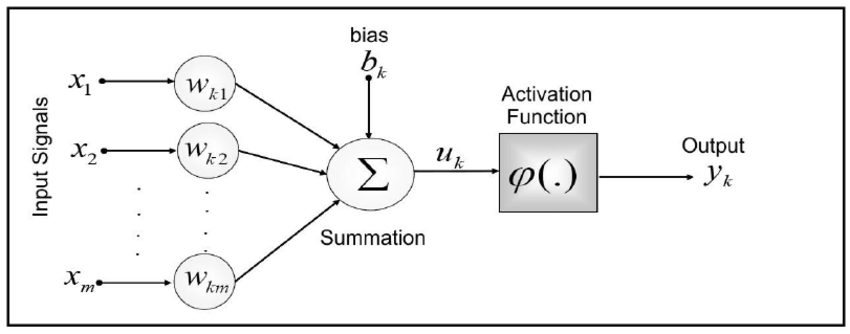
\includegraphics[width= 0.7\linewidth]{bab2/ANN 2.png}
      \caption{\textit{Artificial Neural Network}}
      \label{fig: ANN}
    \end{center}
\end{figure}

Nilai sebuah output dari \textit{artificial neural network} juga
dipengaruhi oleh bias. Bias pada sebuah model dapat disebabkan oleh dataset awal atau karena kurangnya
pemprosesan data. Sebagai contoh, data untuk membedakan gambar kucing dan anjing digunakan untuk membangun
sebuah model klasifikasi anjing dan kucing, terdapat 500 gambar data anjing yang digunakan, namun
hanya ada 20 gambar kucing yang digunakan. Tentunya dengan dataset ini, model akan cenderung
memprediksi atau mengklasifikasikan gambar menjadi kelas anjing. Bias yang sama pun juga dapat terjadi
pada sebuah prediksi nilai atau klasifikasi teks. Bias yang dapat terjadi lainnya adalah jika model
memiliki data \textit{train} duplikat. Hal ini dapat memberikan \textit{overfitting} 
karena saat diuji coba dengan gambar yang berbeda, nilai performa model menurun.

Pada sebuah \textit{artificial neural network} terdapat beberapa \textit{activation function} yang 
dapat diaplikasikan. \textit{Activation function} mengatur apakah sebuah neuron harus diaktifkan dan nilainya
digunakan atau tidak. Hal ini berguna dalam memprediksi ataupun mengkalsifikasi suatu hal berdasarkan
nilai dari input \textit{artificial neural network} dimana dengan sebuah \textit{threshold}, nilai input
tertentu dapat memberikan nilai output 0 jika data input dianggap tidak berguna dalam memprediksi. Terdapat tiga \textit{activation function} yang umum digunakan yaitu fungsi sigmoid, ReLu, dan TanH.

\begin{itemize}
    \item \textbf{Sigmoid}
    \begin{equation}
        h_ \theta (x) =  \frac{\mathrm{1} }{\mathrm{1} + e^- \theta^Tx }
    \end{equation}

    \begin{figure}[h!]
        \begin{center}
          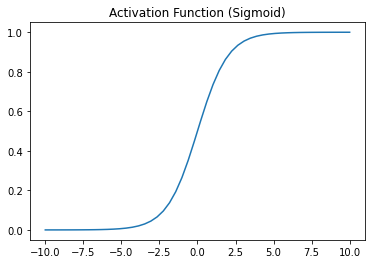
\includegraphics[width= 0.5\linewidth]{bab2/21. sigmoid.png}
          \caption{Fungsi Sigmoid}
          \label{fig: Sigmoid}
        \end{center}
    \end{figure}

    Fungsi aktivasi yang umum digunakan pertama adalah fungsi sigmoid, fungsi sigmoid memberikan
    nilai dibawah 0,5 pada nilai input negatif, dan nilai 0 pada nilai negatif yang lebih kecil dari
    -5. Sebaliknya, fungsi ini memberikan nilai diatas 0,5 pada nilai positif dan nilai 1 pada nilai
    input diatas 5. Jika nilai input 0, maka fungsi ini akan memberikan nilai 0,5. Nilai maksimal dari fungsi
    ini adalah 1 dan nilai minimalnya adalah 0.

    \item \textbf{Tanh}
    \begin{equation}
        \tanh{x}
    \end{equation}

    \begin{figure}[h!]
        \begin{center}
          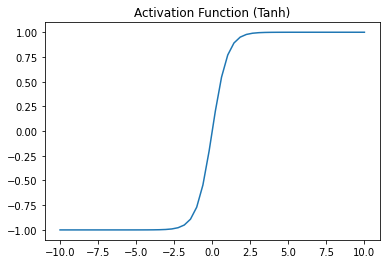
\includegraphics[width= 0.5\linewidth]{bab2/22. tanh.png}
          \caption{Fungsi Tanh}
          \label{fig: Tanh}
        \end{center}
    \end{figure}

    Fungsi aktivasi kedua adalah tanh, jika sebelumnya fungsi sigmoid memiliki nilai minimal 0, maka
    pada fungsi tanh, nilai minimal yang dimiliki adalah -1 sedangkan nilai maksimal yang dimiliki adalah 1. 
    Fungsi tanh akan memberikan nilai negatif pada input negatif, nilai 0 pada input 0, dan nilai 
    positif pada input positif.

    \item \textbf{ReLu}
    \begin{equation}
        Relu(x) = max(0,x)
    \end{equation}

    \begin{figure}[h!]
        \begin{center}
          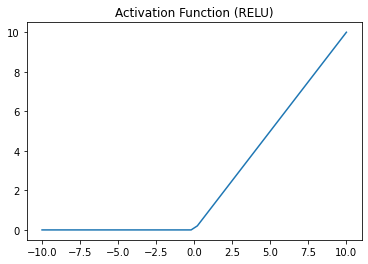
\includegraphics[width= 0.5\linewidth]{bab2/20. Relu.png}
          \caption{Fungsi ReLu}
          \label{fig: ReLu}
        \end{center}
    \end{figure}

    Fungsi aktivasi ketiga adalah ReLu, fungsi ReLu memiliki nilai minimal 0 namun tidak mempunyai nilai maksimal. 
    ReLu merupakan suatu fungsi aktivasi linear yang sering digunakan dalam mengklasifikasi gambar.
    Fungsi ReLu akan memberikan nilai 0 pada input 0 dan negatif sedangkan pada input positif, ReLu akan memberikan
    output nilai input itu sendiri. Terdapat juga fungsi ReLu yang memberikan nilai negatif pada input
    negatif, fungsi ReLu yang memberikan nilai negatif disebut dengan leaky ReLu.

\end{itemize}

\section{\textit{Convolutional Neural Network}}
\textit{Convolutional neural network} adalah sebuah jaringan \textit{neural network} yang memanfaatkan
operasi matematika konvolusi dan pooling dalam memproses matriks atau tensor inputnya.
\textit{Convolutional neural network} umum digunakan dalam pengolahan citra karena dapat mengekstrak
fitur pada gambar dengan baik.

\begin{figure}[h!]
    \begin{center}
      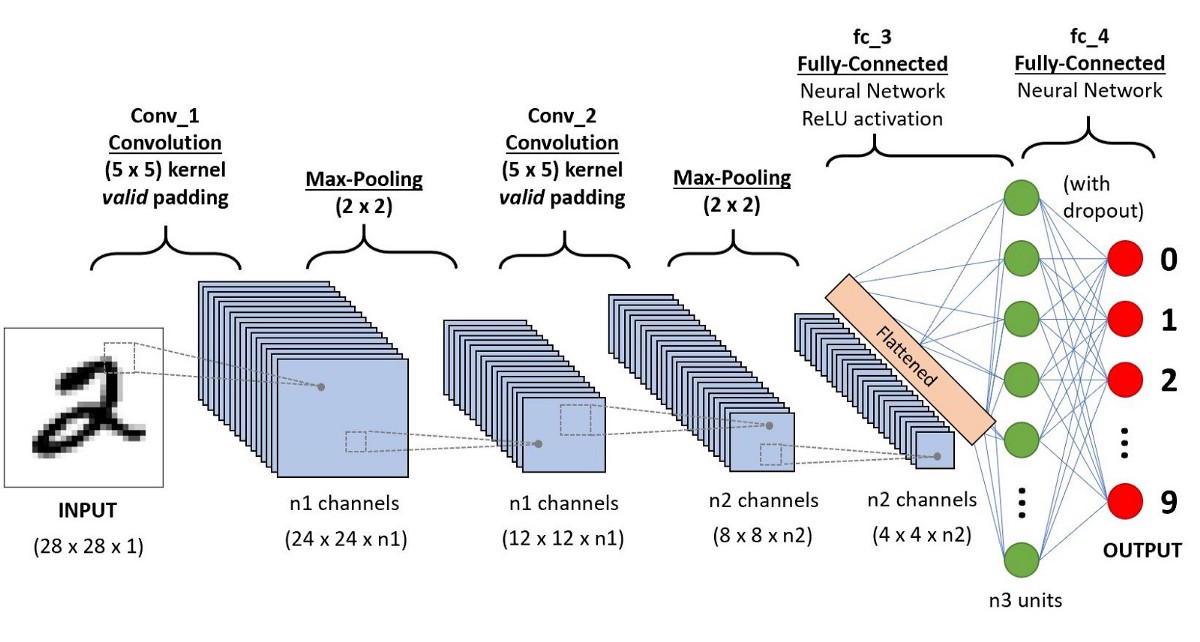
\includegraphics[width= 0.75\linewidth]{bab2/Contoh Arsitektur CNN.jpeg}
      \caption{Contoh Arsitektur CNN}
      \label{fig: Arsi CNN}
    \end{center}
\end{figure}

\subsection{Konvolusi}
Konvolusi merupakan suatu operasi matematika yang sering dilakukan untuk melakukan pemprosesan gambar.
Konvolusi dilakukan untuk mengekstrak fitur-fitur pada gambar agar perbedaan nilai pada fitur yang
ingin diekstrak semakin besar dan fitur yang akan diproses menjadi lebih mudah dilihat oleh komputer
karena memiliki nilai yang lebih besar serta memori atau ukuran gambar yang lebih kecil. Proses konvolusi
dimulai dengan mempersiapkan sebuah matriks kernel yang berukuran sama atau kurang dari ukuran matriks
gambar yang ingin diproses. Umumnya matriks kernel ini berukuran 3x3. Kemudian pada matriks awal akan 
diambil sebuah bagian dari matriks yang berukuran sama kemudian dikalikan dengan matriks kernel. Hasil
dari perkalian tersebut kemudian dijumlahkan menjadi satu nilai yang menjadi satu elemen pada matriks
yang baru / matriks dari hasil konvolusi. Pada CNN, nilai kernel matriks ini akan didefinisikan oleh
\textit{neural network}.

\begin{figure}[h!]
    \begin{center}
      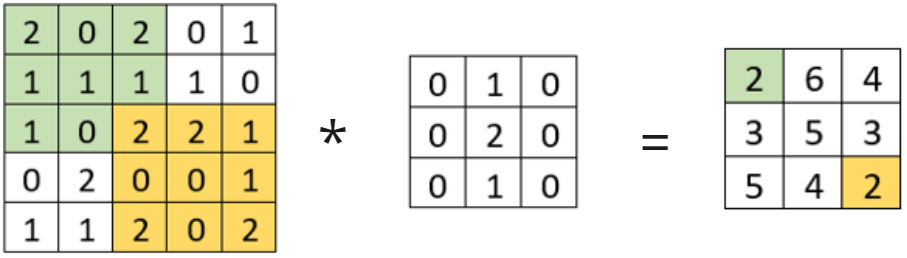
\includegraphics[width= 0.7\linewidth]{bab2/Convolution.png}
      \caption{Konvolusi}
      \label{fig: Konvolusi}
    \end{center}
\end{figure}

\subsection{\textit{Pooling}}
\textit{Pooling} merupakan suatu operasi matematika yang digunakan untuk memperkecil ukuran matriks dengan memilih
atau memproses nilai pada matriks. \textit{Pooling} pada pemprosesan citra umumnya dilakukan pada setiap bagian matriks
dengan ukuran 2x2 atau 3x3. Contoh dari operasi \textit{pooling} dapat dilihat pada gambar \ref{fig: Pooling}.
Terdapat beberapa jenis \textit{pooling}, dan beberapa \textit{pooling} yang sering digunakan ialah
\textit{max pooling} dan \textit{average pooling}. \textit{Max pooling} mengambil elemen matriks dengan
nilai tertinggi pada suatu sekumpulan matriks sesuai dengan ukuran yang sudah didefinisikan. Misalnya 
jika matriks berukuran 4x4 mengalami proses \textit{pooling} 2x2, maka hasil dari matriks tersebut adalah
1 elemen matriks dari setiap bagian matriks berukuran 2x2 pada matriks 4x4 dimana elemen yang telah diproses
tidak diproses kembali. Sehingga hasil dari matriks 4x4 yang mengalami proses \textit{pooling} 2x2
adalah matriks berukuran 2x2.

Sedangkan jenis \textit{pooling} yang sering digunakan lainnya adalah \textit{average pooling}
dimana jika sebelumnya pada \textit{max pooling} elemen dengan nilai tertinggi yang dipilih, maka
pada \textit{average pooling} maka akan dipilih nilai rata-rata dari \textit{pooling} tersebut. Jika
misalnya pada sebuah matriks dilakukan proses \textit{pooling} 2x2, maka rata-rata dari empat elemen
dari bagian matriks yang berukuran 2x2 akan menjadi elemen dari matriks hasil \textit{pooling}. Perbedaan 
jenis \textit{pooling} tidak mempengaruhi ukuran matriks dari hasil pemprosesan \textit{pooling}, namun
tentunya mempengaruhi nilai hasil \textit{pooling}.

\begin{figure}[h!]
    \begin{center}
      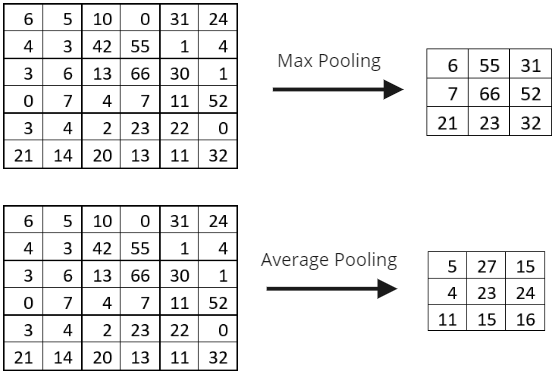
\includegraphics[width= 0.7\linewidth]{bab2/Pooling.png}
      \caption{Contoh \textit{Pooling} 2x2}
      \label{fig: Pooling}
    \end{center}
\end{figure}

\section{Deteksi Objek}
Deteksi objek (\textit{object detection}) adalah suatu teknik pada \textit{computer vision} dimana
suatu komputer dapat mengenali dan mengetahui lokasi dari objek yang menjadi fokus secara otomatis
layaknya manusia. \textit{Object detection} dapat dicapai dengan penggunaan \textit{deep learning}.
Salah satu kelemahan dalam pembuatan sebuah komputer pendeteksi objek adalah, tingginya daya komputasi
yang diperlukan dan dalam mendeteksi \textit{multiple class} membutuhkan dataset yang banyak sehingga
kebutuhan \textit{storage} pun meningkat. Sebagian besar detektor objek beroperasi dengan memilih 
sekumpulan kandidat region yang mengandung objek fokus dari gambar dan mengklasifikasikannya ke dalam 
daerah objek \textit{foreground} dan daerah yang tidak memiliki objek (biasanya disebut sebagai latar belakang). 
Pada dasarnya, pendekatan tersebut dapat mengurangi tugas deteksi objek menjadi tugas klasifikasi gambar yang lebih sederhana. 
Kandidat daerah yang akan diklasifikasikan dapat diperoleh dengan mudah dengan cara 
\textit{brute force} dengan menggeser jendela m × n di atas gambar atau yang sering disebut algoritma 
\textit{sliding window}. Mengikuti metode ekstraksi fitur dari \textit{sliding window}, terdapat metode dimana setiap 
\textit{region} akan dinilai berdasarkan kerapatan tepi, ukuran, dan lokasi pada objek dan metode lain
dimana gambar tersebut akan disegmentasi terlebih dahulu menjadi beberapa bagian kemudian mengkombinasikannya
berdasarkan kemiripannya. Salah satu metode yang mensegmentasi gambar dan mengelompokkan gambar tersebut adalah
\textit{selective search} \cite{UijlingsIJCV2013}. 

Dalam menunjukkan lokasi objek, seringkali sebuah \textit{bounding box} dibentuk untuk menandakan lokasi
dari objek yang menjadi fokusan. \textit{Bounding box} juga digunakan dalam metode \textit{selective search}
untuk menjadi kandidat objek deteksi. Kandidat objek harus meliputi semua objek pada gambar sehingga
tidak ada objek yang terlewati dan objek-objek tersebut dapat diklasifikasi. Di sisi lain
\textit{bounding box} pada kandidat objek yang terlalu banyak dapat mengakibatkan \textit{bounding box}
menimpa satu sama lain pada satu objek yang sama. 

Untuk mengatasi hal ini dan mengambil \textit{bounding box}
terbaik, maka suatu metode yang dinamakan \textit{non-max supression} per diaplikasikan. Pertama-tama, 
semua \textit{bounding box} perlu dicek apakah menimpa objek yang sama atau tidak, hal ini dapat dilakukan
dengan menganalisa koordinat dari \textit{bounding box}, kemudian nilai \textit{interference over union} (IoU)
pada \textit{bounding box} yang meliputi objek yang sama akan diperiksa, jika nilai IoU pada
\textit{bounding box} di atas 0,5 maka \textit{bounding box} tersebut tidak dibuang kemudian jika terdapat
beberapa \textit{bounding box} yang memiliki nilia IoU di atas 0,5, maka akan dipilih \textit{bounding box}
dengan nilai IoU terbesar \cite{hawking1988}.

\begin{figure}[h!]
    \begin{center}
      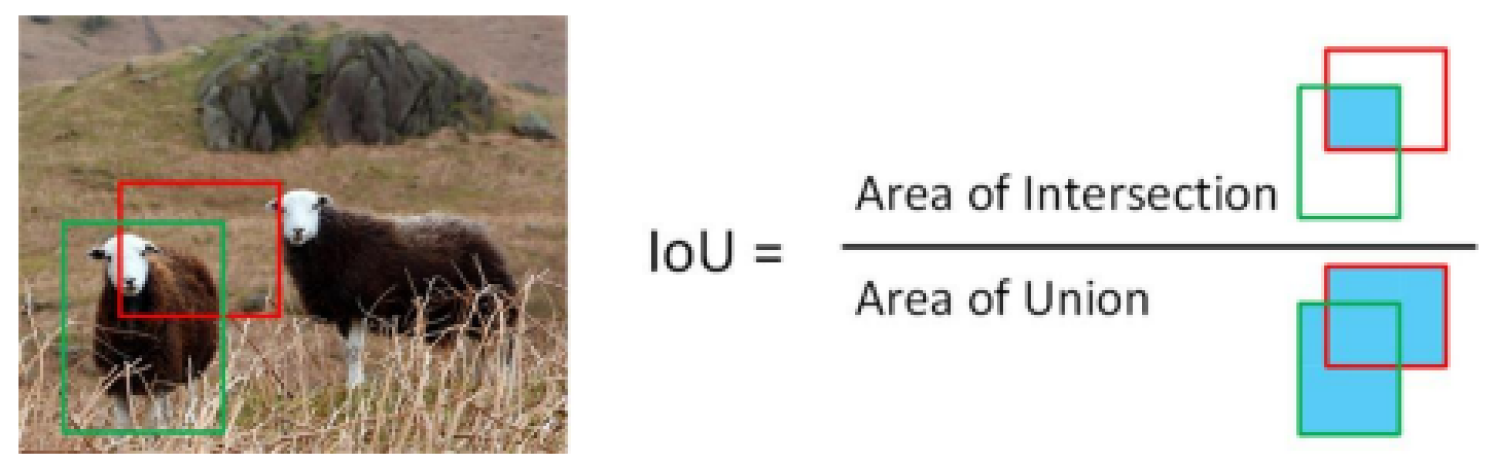
\includegraphics[width= 1\linewidth]{bab2/IoU.png}
      \caption{\textit{Intersect over Union}}
      \label{fig: IoU}
    \end{center}
\end{figure}

\subsection{\textit{Two-Stage Object Detectors}}
\textit{Two-stage object detectors} adalah suatu prinsip pada deteksi objek dengan mengikuti prinsip
mencari daerah kandidat atau daerah proposal. Kemudian daerah proposal tersebut akan dideteksi secara
lebih lanjut. Seperti namanya \textit{two stage object detectors} memiliki dua tahapan detektor
dimana tahap pertama adalah pemberian proposal dan tahap kedua adalah klasifikasi dan deteksi objek
\cite{hawking1988}.

Salah satu contoh algoritma yang menerapkan \textit{two-stage object detectors} adalah R-CNN. 
Pada R-CNN, algoritma pencarian selektif mengekstrak \textit{{region proposal}}
dari gambar, yang kemudian akan menghasilkan satu set kandidat objek yang diberi \textit{bounding box}. 
Setelah memperoleh proposal wilayah, jaringan saraf convolutional digunakan sebagai ekstraktor fitur 
di atas setiap proposal yang diekstraksi, menghasilkan \textit{feature} gambar dari setiap proposal. 

\begin{figure}[h!]
    \begin{center}
      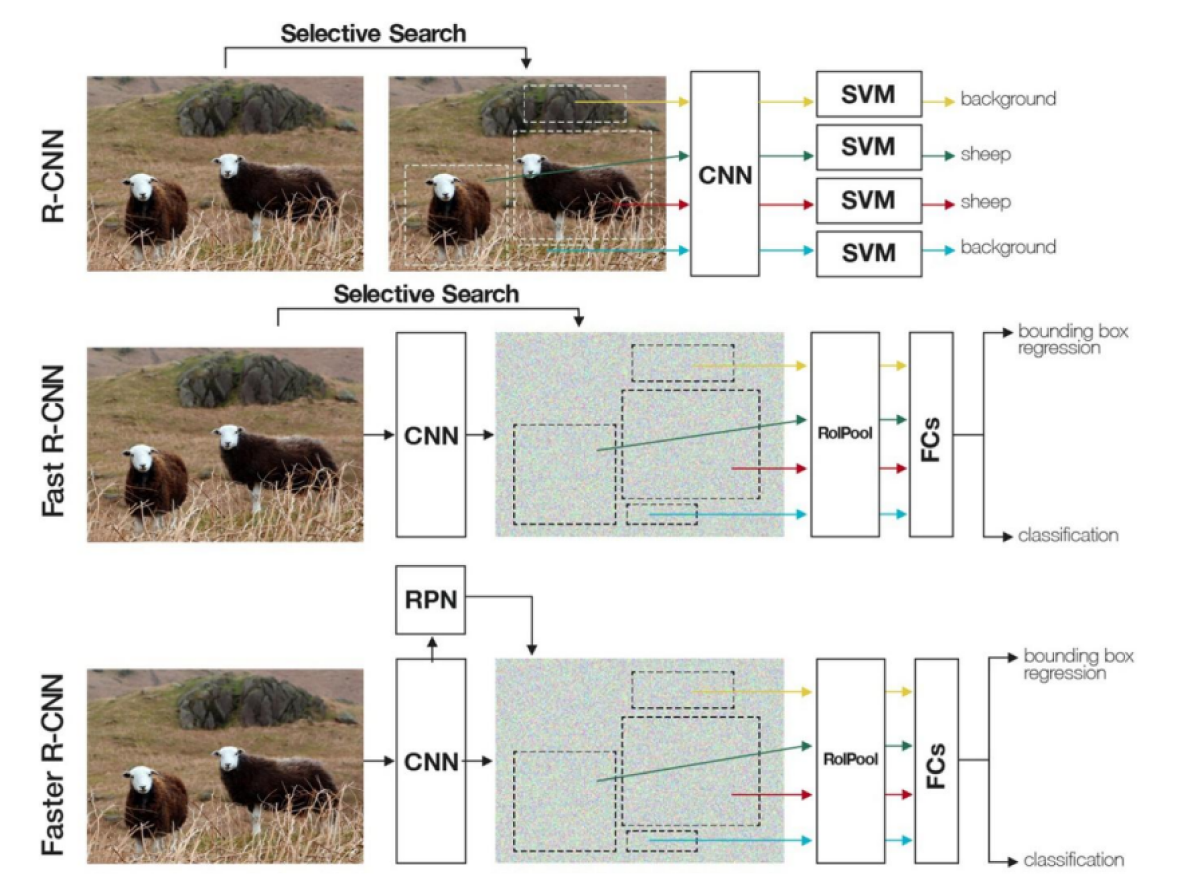
\includegraphics[width= 1\linewidth]{bab2/Two stage.png}
      \caption{Contoh \textit{Two Stage Detector}}
      \label{fig: Two Stage Detector}
    \end{center}
\end{figure}

Secara khusus, untuk setiap gambar, pembuatan \textit{region proposal} yang membentuk sebuah
\textit{bounding box} suatu objek harus mempunyai IoU melebihi nilai ambang (0,5 umumnya digunakan). Hal ini 
dianggap sebagai contoh positif untuk kelas objek yang sesuai,
sementara proposal yang memiliki nilai IoU
lebih rendah dari ambang (0,5) dianggap sebagai contoh negatif untuk semua kelas objek dan dianggap 
sebagai latar belakang (bukan objek). Setelah proposal dibentuk, maka algoritma lanjutan yang menggunakan SVM akan memprediksi kelas pada
objek yang menjadi proposal dan objek proposal yang dipilih adalah proposal yang memiliki IoU tertinggi
dari suatu objek yang tumpang tindih.

\subsection{\textit{Single-Stage Object Detector}}
Selain \textit{two-stage object detector} adapula deteksi objek dengan menggunakan \textit{single stage}.
Pada metode ini, \textit{region proposal} tidak dibentuk sehingga objek dideteksi dan diklasifikasi
secara langsung. Tentunya karena tidak memerlukan tahapan pemebentukan \textit{region proposal} maka
algoritma yang menggunakan metode ini memproses gambar lebih cepat dan mendeteksi objek secara lebih cepat.
Beberapa contoh dari penerapan \textit{Single-stage object detector} adalah algoritma 
\textit{Single Shot Detector (SSD)} dan \textit{You Only Look Once (YOLO)} 
\cite{https://doi.org/10.48550/arxiv.1506.02640}. 

YOLO menggunakan 24 lapis jaringan konvolusi untuk ekstraksi fitur, diikuti oleh 2 lapisan yang 
\textit{fully connected}. 20 lapisan konvolusional pertama dilatih pada ImageNet untuk klasifikasi, 
dan setelah menambahkan lapisan yang tersisa, model selanjutnya dilatih untuk mendeteksi objek. 
YOLO membagi gambar menjadi sel menjadi ukuran SxS (umumnya 7x7) dan memprediksi kotak pembatas 
bersama dengan skor \textit{confidence}, serta distribusi probabilitas kelas untuk setiap sel grid. 
Setiap pembatas kotak diberikan parameter oleh titik pusat kotak relatif terhadap sel grid, yang
lebar dan tingginya relatif terhadap keseluruhan gambar \cite{hawking1988}. Skor kepercayaan dari kotak pembatas secara 
formal didefinisikan sebagai IoU antara kotak pembatas yang diprediksi dan
kotak kebenaran dasar yang sesuai. Perhatikan bahwa tidak seperti Faster R-CNN yang memprediksi 
offset dari kotak jangkar, YOLO memprediksi koordinat kotak pembatas akhir secara langsung.

\begin{figure}[h!]
    \begin{center}
      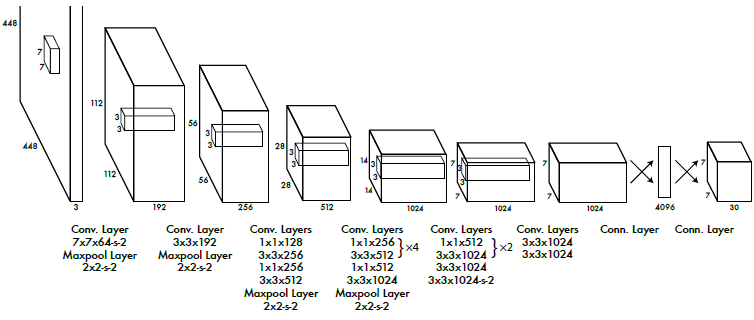
\includegraphics[width= 1\linewidth]{bab2/Yolo Archi.png}
      \caption{Arsitektur YOLO \cite{YOLOYOLA}}
      \label{fig: Archi YOLO}
    \end{center}
\end{figure}

\section{Algoritma Deteksi Objek Mask R-CNN}

Mask R-CNN \cite{https://doi.org/10.48550/arxiv.1703.06870} adalah jaringan saraf dalam untuk memecahkan masalah segmentasi instans. 
Dengan kata lain, dapat memisahkan objek yang berbeda dalam gambar atau video. 
Dengan memberikan input gambar, Mask R-CNN akan memberikan kotak pembatas objek, kelas, dan \textit{mask}.
Mask R-CNN merupakan pengembangan dari \textit{faster R-CNN} dimana sebuah \textit{mask} akan dibentuk
dalam mendeteksi objeknya.

Saat ini Mask R-CNN pertama kali dikemukakan pada tahun 2017 dan sejak saat itu menjadi salah satu algoritma
deteksi objek yang terkenal dan menarik untuk diimplementasikan. Pengaplikasian Mask R-CNN sudah dilakukan
di berbagai penelitian seperti deteksi algae, deteksi sel kanker, deteksi pneumonia, dan masih banyak lagi.
Mask R-CNN adalah salah satu algoritma yang memanfaatkan \textit{two stage detector} dalam mendeteksi objek
dan dapat mensegmentasi objek hingga level piksel.

\begin{figure}[h!]
    \begin{center}
      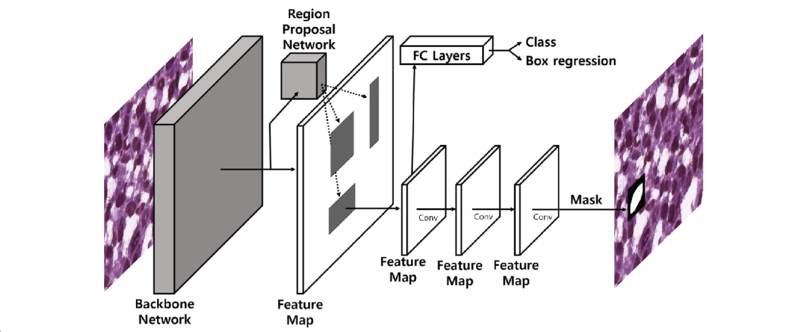
\includegraphics[width= 1\linewidth]{bab2/Mask R-CNN Archi.png}
      \caption{Arsitektur Mask R-CNN \cite{Mask-archi}}
      \label{fig: Mask RCNN Archi}
    \end{center}
\end{figure}

Ada dua tahap Mask RCNN. Pertama, menghasilkan proposal tentang wilayah di mana mungkin terdapat objek 
berdasarkan gambar input. Kedua, memprediksi kelas objek, menyempurnakan kotak pembatas dan 
menghasilkan \textit{mask} di tingkat piksel objek berdasarkan proposal tahap pertama.
Tentunya seperti algoritma deteksi objek lainnya, pelabelan kelas dan penunjukkan lokasi objek
yang ingin dideteksi dibutuhkan pada data \textit{train}. Mask R-CNN mengambil data kelas dan objek
yang telah diberikan \textit{mask} kemudian mengekstrak fitur-fitur pada gambar data \textit{train}.

Dalam mengambil target untuk melatih proses pengekstrakan fitur secara lebih dalam, maka sebuah target
perlu dibentuk. Pada hal ini, Mask R-CNN memanfaatkan \textit{anchor box} untuk memberikan perkiraan
dimanakah objek yang perlu dideteksi berada, jika \textit{anchor box} mempunyai IoU lebih dari sama dengan 0,5
dengan \textit{bounding box} awal maka \textit{anchor box} tersebut disimpan untuk menjadi target
kecuali jika \textit{bounding box} tersebut \textit{overlap} dengan \textit{anchor box} lain, maka
\textit{anchor box} yang mempunyai nilai IoU terbaik yang akan dipilih menjadi target.
\textit{Anchor box} yang disimpan akan menjadi target bagi \textit{backbone} untuk mengekstrak fitur
menggunakan neural network.

Pengekstrakan fitur dimulai dengan proses konvolusi pada jaringan \textit{backbone}. Umumnya
\textit{backbone} yang digunakan pada algoritma ini adalah \textit{Residual Network} atau yang 
disingkat ResNet. ResNet merupakan sebuah jaringan yang dibentuk oleh berbagai konvolusi, proses
\textit{pooling}, dan lapisan neural network. Saat ini terdapat lima layer atau lima jenis ResNet
yang dibedakan menurut jumlah layernya. Untuk 18 layer ResNet, jaringan tersebut disusun oleh 1 layer
konvolusi 7x7-64 neural network, kemudian proses pooling 3x3 (tidak dihitung sebagai layer), kemudian
4 layer konvolusi 3x3-64 neural network, 4 layer konvolusi 3x3-128 neural network, 4 layer konvolusi 3x3-256 neural network,
4 layer konvolusi 3x3-512 neural network, dan layer terakhir adalah \textit{fully connected layer}
atau yang disebut sebagai FC dengan \textit{softmax function} untuk memberikan output dengan berbagai kelas.

Sedangkan pada contoh layer ResNet yang lain, contohnya ResNet 101, layer pada ResNet akan terdiri
dari 101 layer dan dapat dilihat pada gambar \ref{fig: Resnet macam}. Jaringan pada \textit{backbone}
akan menghasilkan sebuah \textit{Region Proposal Network (RPN)} yang merupakan hasil dari \textit{anchor box}
yang mempunyai IoU lebih besar dari 0,5 dengan \textit{bounding box} asli. Dan \textit{feature map} 
yang memuat data hasil dari konvolusi dan pelatihan \textit{neural network} yang berada pada \textit{backbone}.

\begin{figure}[h!]
    \begin{center}
      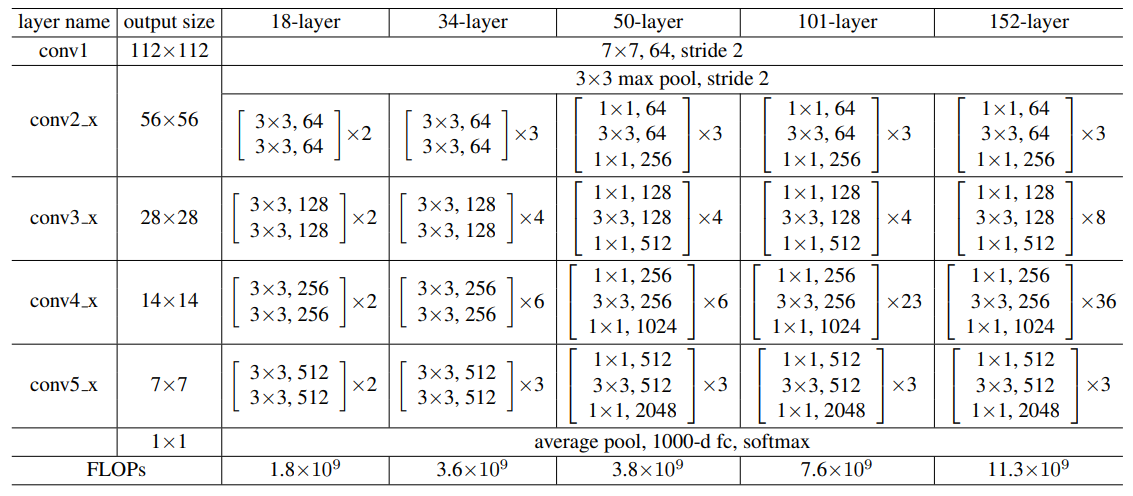
\includegraphics[width= 1\linewidth]{bab2/ResNet 101-2.png}
      \caption{Macam - macam \textit{Residual Network (ResNet)} \cite{https://doi.org/10.48550/arxiv.1512.03385}}
      \label{fig: Resnet macam}
    \end{center}
\end{figure}

Hasil dari ekstraksi fitur oleh jaringan \textit{backbone} berupa sebuah \textit{heatmap} hasil konvolusi
dari algoritma ResNet yang disebut \textit{feature map}, hal ini akan memudahkan tahapan memprediksi kelas, ukuran objek, dan pembuatan \textit{mask}.
Dalam memprediksi kelas dan memberikan \textit{bounding box} pada objek, \textit{feature map} diproses
menggunakan \textit{fully connected layer}. \textit{Fully connected layer} merupakan sebuah lapisan
\textit{neural network} yang mengkoneksikan setiap neuron pada satu layer ke setiap neuron pada layer selanjutnya
umumnya digunakan pada lapisan output untuk memberikan kelas. Selain itu, \textit{feature map} juga digunakan
untuk membentuk \textit{mask} menggunakan lapisan konvolusi.

Dalam melatih model Mask R-CNN, terdapat beberapa metriks yang perlu diketahui untuk mengetahui
seberapa bagus proses \textit{training} yang biasanya dinyatakan dalam metriks loss. dalam Mask RCNN
terdapat 5 metriks loss yang dibedakan menjadi loss RPN dan loss MRCNN. Loss RPN merupakan loss yang terjadi pada pembuatan dan pelatihan jaringan \textit{backbone}
dalam memberikan \textit{region proposal}. Loss RPN dibedakan menjadi dua yaitu loss RPN \textit{bounding box}
dan loss RPN \textit{class}. Loss RPN \textit{bounding box} merupakan loss yang terjadi untuk mengetahui
seberapa besar perbedaan \textit{bounding box} pada objek yang diprediksi dengan \textit{bounding box}
aslinya. Sedangkan pada Loss RPN class merupakan loss yang terjadi saat ada kesalahan prediksi objek menjadi
\textit{background} ataupun prediksi \textit{background} menjadi objek.

\begin{equation}
    \label{eq :loss}
    \mathcal{L} = \mathcal{L}_\text{RPN-cls} + \mathcal{L}_\text{RPN-box}
\end{equation}

\begin{equation}
    \label{eq :cls_loss}
    \mathcal{L}_\text{RPN-cls} (p_i, p^*_i) = - p^*_i \log p_i - (1 - p^*_i) \log (1 - p_i)
\end{equation}

\begin{equation}
    \label{eq :bbox loss}
    \mathcal{L}_\text{RPN-box} = \frac{\lambda}{N_\text{box}} \sum_i p^*_i \cdot L_1^\text{smooth}(t_i - t^*_i)
\end{equation}

Kemudian dalam loss yang sering kali disebut loss MRCNN merupakan loss yang terjadi tahapan setelah
pembuatan \textit{feature map} dan digunakan untuk mengetahui seberapa bagus performa dari output
pada Mask RCNN. Loss MRCNN dibedakan menjadi tiga jenis yaitu loss class, loss bounding box, dan loss mask.
\textit{loss class} adalah loss yang terjadi saat adanya kesalahan prediksi pada kelas objek, jika sebelumnya
pada loss rpn, perbedaan kelas hanyalah objek atau tidak (\textit{foreground or background}) pada loss
MRCNN, kelas yang diprediksi adalah kelas nama objek yang diteliti. Kemudian pada loss bounding box
merupakan hal yang hampir sama pada loss rpn bounding box, perbedaannya ialah, loss ini merupakan
perbandingan output akhir prediksi dengan data awal. Kemudian loss terakhir adalah loss mask yang merupakan
metriks untuk melihat seberapa berbedanya mask yang dibentuk dengan mask data awal. Dibawah ini merupakan
persamaan dari loss MRCNN.

\begin{equation}
    \label{eq :loss}
    \mathcal{L} = \mathcal{L}_\text{cls} + \mathcal{L}_\text{box} + \mathcal{L}_\text{mask}
  \end{equation}
  
  \begin{equation}
    \label{eq:other Loss}
    \mathcal{L}_\text{fr} = \mathcal{L}_\text{cls} + \mathcal{L}_\text{box}
  \end{equation}
  
  \begin{equation}
    \mathcal{L}_\text{fr}(\{p_i\}, \{t_i\}) = \frac{1}{N_\text{cls}} \sum_i \mathcal{L}_\text{cls} (p_i, p^*_i) + \frac{\lambda}{N_\text{box}} \sum_i p^*_i \cdot L_1^\text{smooth}(t_i - t^*_i)
  \end{equation}
  
  \begin{equation}
    \label{eq :cls_loss}
    \mathcal{L}_\text{cls} (p_i, p^*_i) = - p^*_i \log p_i - (1 - p^*_i) \log (1 - p_i)
  \end{equation}
  
  \begin{equation}
    \label{eq :bbox loss}
    \mathcal{L}_\text{box} = \frac{\lambda}{N_\text{box}} \sum_i p^*_i \cdot L_1^\text{smooth}(t_i - t^*_i)
  \end{equation}
  
  \begin{equation}
    \label{eq :mask loss}
    \mathcal{L}_\text{mask} = - \frac{1}{m^2} \sum_{1 \leq i, j \leq m} \big[ y_{ij} \log \hat{y}^k_{ij} + (1-y_{ij}) \log (1- \hat{y}^k_{ij}) \big]
\end{equation}

\section{Metode Analisa Performa Model}
Terdapat beberapa metode yang bisa dilakukan untuk mengetahui apakah suatu model memiliki akurasi yang cukup. 
Penelitian ini menggunakan beberapa formula yang sudah ditentukan seperti \textit{recall, precision, f1-score} 
dan \textit{confusion matrix}.

\subsection{\textit{Recall}}
\textit{Recall} adalah formula yang harus digunakan ketika kita memiliki data yang tidak seimbang. Berbeda 
dengan akurasi yang hanya menghitung persentase model memprediksi hasil yang sesuai dengan label secara 
keseluruhan, \textit{recall} akan menghitung rasio nilai yang diprediksi positif dengan total keseluruhan 
nilai yang positif \cite{metrics_ml}. Rumus \ref{form:recall} merupakan rumus untuk menghitung \textit{recall}.

\begin{equation}
    Recall = \frac{TP}{TP+FN}
    \label{form:recall}
\end{equation}

\subsection{\textit{Precision}}
Seringnya, kita tidak hanya melihat tingkat akurasi suatu model hanya dengan besaran \textit{recall} maupun 
tingkat akurasi nya. \textit{Precision} adalah formula untuk menghitung rasio dari prediksi TP (\textit{True 
Positive}) yang benar dengan keseluruhan prediksi. Apabila prediksi yang dilakukan oleh model kita ternyata 
memiliki tingkat presisi yang tinggi namun memiliki tingkat \textit{recall} yang rendah, ada kemungkinan model 
tidak dapat melakukan prediksi pada data yang bersifat negatif \cite{metrics_ml}. Rumus \ref{form:precision} 
merupakan rumus untuk menghitung nilai dari \textit{precision} suatu model.

\begin{equation}
    Precision = \frac{TP}{TP+FP}
    \label{form:precision}
\end{equation}

Baik \textit{recall} maupun \textit{precision} merupakan nilai yang cukup penting terutama pada data yang tidak 
seimbang. Terdapat 3 kelfndisi yang umum terjadi pada saat membandingkan antara \textit{precision} dengan 
\textit{recall}.

\begin{itemize}
    \item \textit{Recall} tinggi, \textit{Precision} rendah
          Sebagian besar data positif dapat diprediksi dengan benar (\textit{False Negative} yang Rendah), 
          namun hanya ada sebagian kecil data negatif yang diprediksi dengan benar (\textit{True Negative} 
          rendah).

    \item \textit{Recall} rendah, \textit{Precision} tinggi
          Hasil prediksi model memiliki banyak sekali prediksi negatif (\textit{False Negative} tinggi), 
          namun apabila digunakan untuk memprediksi data positif, maka hasil prediksi sebagian besarnya adalah 
          benar (\textit{False Positive} rendah).

    \item \textit{Recall} tinggi, \textit{Precision} tinggi
          Merupakan hasil yang ideal dalam pembuatan model pembelajaran mesin. Disini didapatkan bahwa baik 
          hasil prediksi untuk data positif maupun hasil prediksi untuk data negatif sebagian besarnya adalah 
          benar (\textit{True Positive} dan \textit{True Negative} tinggi).

\end{itemize}

\subsection{mAP@50}
Dalam mengukur performa sebuah deteksi objek, sebuah threshold IoU 0,5 merupakan parameter yang umum digunakan
dimana jika IoU deteksi bernilai lebih dari sama dengan 0,5, maka dapat dikatakan bahwa deteksi yang
dihasilkan adalah bagus. Adapula parameter performa yang dinamakan \textit{average precission} yang didefinisikan
sebagai luasan dari area di bawah kurva \textit{recall-precission}. Umumnya parameter performa ini ditulis
sebagai mAP@50

\subsection{\textit{F1-Score}}

\textit{F1-Score} adalah besaran yang berasal dari rata - rata harmonik dari \textit{recall} dan 
\textit{precision}. Rata  - rata harmonik dipilih karena akan menghasilkan nilai rata - rata yang lebih rendah 
dalam kondisi tidak seimbang apabila dibandingkan dengan rata - rata aritmatis biasa. Dengan rata - rata seperti 
itu, suatu model dapat menjadi lebih rentan terhadap bias dan memudahkan pada saat pembuatan model 
\cite{metrics_ml}. Rumus \ref{form: f1-score} merupakan rumus untuk menghitung f1-score.

\begin{equation}
    \label{form: f1-score}
    F1-Score = 2 \times \frac{\textit{Recall} \times \textit{Precision}}{\textit{Recall} + \textit{Precision}}
\end{equation}

\subsection{\textit{Confusion Matrix}}

\textit{Confusion Matrix} adalah tabel kesimpulan yang berisi jumlah prediksi baik yang benar maupun yang 
salah dan nilai label baik yang benar maupun salah. Biasanya tabel jenis ini digunakan untuk tugas yang 
bersifat klasifikasi dan berfungsi untuk memvisualisasi bagaimana suatu performa model dalam suatu dataset.

\begin{table}
    \caption{Contoh \textit{Confusion Matrix}}
    \label{tab:cth_confusion_mtrx}
    \centering
    \begin{tabular}{|l|l|l|l|l}
        \cline{1-4}
        \multicolumn{2}{|l|}{\multirow{2}{*}{}} & \multicolumn{2}{l|}{\textbf{Aktual}} &                \\ \cline{3-4}
        \multicolumn{2}{|l|}{}                  & Positif                              & Negatif &      \\ \cline{1-4}
        \multirow{2}{*}{\textbf{Prediksi}}      & Positif                              & TP      & FP & \\ \cline{2-4}
                                                & Negatif                              & FN      & TN & \\ \cline{1-4}
    \end{tabular}
\end{table}

Tabel \ref{tab:cth_confusion_mtrx} adalah contoh tabel \textit{confussion matrix} untuk prediksi dengan 2 label. 
Apabila melihat pada tabel tersebut, dapat terlihat bahwa jumlah prediksi dipecah menjadi masing - masing kelas. 
Diharapkan dengan dipecah menjadi beberapa kelas seperti itu, akan membuat proses pengujian lebih mudah karena 
akan lebih mudah melihat pada saat model memprediksi jenis data apa yang masih memiliki tingkat akurasi yang 
kurang bagus. Terdapat beberapa hal yang harus diketahui untuk dapat memahami sebuah tabel \textit{confussion 
matrix}, yaitu :

\begin{itemize}[nolistsep]
    \item Positif (P)
          Berisi data yang bernilai positif, baik data tersebut beasal dari hasil prediksi maupun data aktual 
          yang didapat dari dataset.

    \item Negatif (N)
          Berisi data yang bernilai negatif, baik data tersebut berasal dari hasil prediksi maupun data aktual 
          yang didapat dari dataset.

    \item \textit{True Positive} (TP)
          Suatu kondisi dimana baik hasil prediksi maupun data aktual sama - sama bernilai positif. Semakin 
          tinggi nilai dari TP, semakin akurat pulalah model yang sudah dibuat.

    \item \textit{False Positive} (FP)
          Suatu kondisi dimana hasil prediksi adalah positif, namun pada data aktual bernilai negatif. 
          Biasanya, semakin tinggi nilai dari FP ini, maka model semakin memilki kecenderungan untuk 
          mengeluarkan nilai positif dibanding negatif atau terjadinya bias pada model.

    \item \textit{True Negative} (TN)
          Suatu kondisi dimana hasil prediksi dan data aktual bernilai negatif. Semakin tinggi nilai FN 
          berarti semakin akurat model yang sudah dibuat.

    \item \textit{False Negative} (FN)
          Suatu kondisi dimana hasil prediksi adalah negatif, namun pada data aktual bernilai positif. 
          Biasanya, semakin tinggi nilai dari TN ini, maka model semakin memiliki kecenderungan untuk 
          mengeluarkan nilai negatif dibanding positif.

\end{itemize}

%%%%%%%%%%%%%%%%%%%%%%%%%%%%%%%%%%%%%%%%%%%%%%%%%%%%%%%%%%




	\cleardoublepage
	\chapter{METODOLOGI}
\label{sec:chap3_metodologi}

\section*{ }
% Ubah bagian-bagian berikut dengan isi dari desain dan implementasi
Penelitian ini dilaksanakan sesuai dengan desain sistem berikut dengan implementasinya. 
Desain sistem merupakan konsep dari pembuatan dan perancangan infrastruktur dan kemudian diwujudkan dalam 
bentuk blok-blok alur yang harus dikerjakan. Sedangkan untuk bagian implementasi merupakan pelaksanaan teknis 
untuk setiap blok pada desain sistem.

\begin{figure}[h!]
	\begin{center}
	  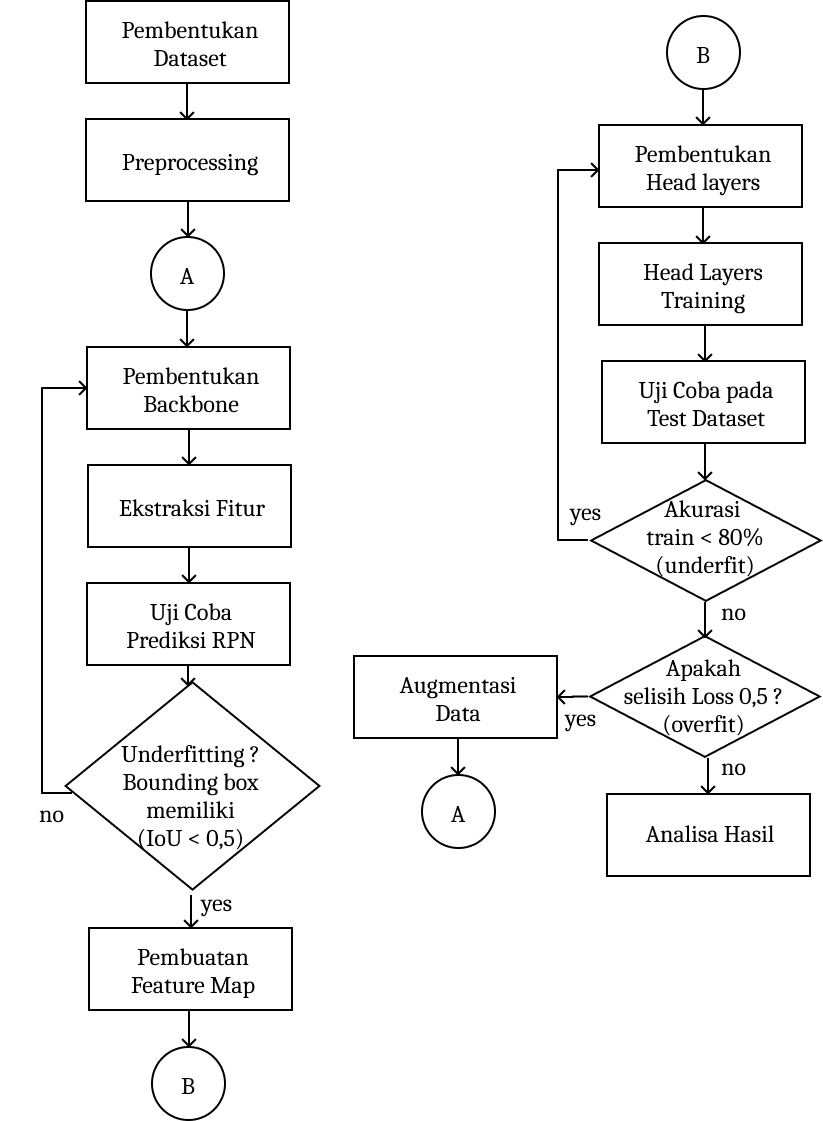
\includegraphics[width= 0.8\linewidth]{bab3/Flow Chart.png}
	  \caption{Bagan Umum Metodologi Penelitian}
	  \label{fig: base_method_1}
	\end{center}
\end{figure}


  Gambar \ref{fig: base_method_1} merupakan bagan yang menunjukkan secara garis besar bagaimana proses pembentukan model
  pada penelitian ini. Penelitian dimulai dengan pembentukan dataset, kemudian dilanjutkan dengan proses \textit{preprocessing}.
  Setelah pembentukan jaringan \textit{backbone}, maka akan dilanjutkan dengan proses ekstraksi fitur menggunakan jaringan
  \textit{backbone} yang telah dibentuk. Kemudian jaringan \textit{backbone} tersebut akan menghasilkan \textit{regional proposal network}
  dan prediksi \textit{bounding box}. Jika model tidak dapat mendeteksi \textit{bounding box} dengan baik dengan kata lain,
  kemiripan \textit{bounding box} yang diprediksi memiliki irisan (IoU) kurang dari 0,5 dengan \textit{bounding box} asli, maka
  jaringan \textit{backbone} perlu dikonfigurasi ulang menggunakan model \textit{backbone} yang berbeda. Kemudian jika model
  \textit{backbone} telah memberikan \textit{bounding box} yang sesuai, maka model \textit{backbone} dapat digunakan untuk
  menghasilkan \textit{feature map}.

  Setelah \textit{feature map} dibentuk, maka \textit{head layers} dibentuk untuk memprediksi kelas dan \textit{bounding box} serta 
  menggenerasi \textit{mask}. Setelah itu lapisan jaringan pada \textit{head} perlu dilatih agar dapat mendeteksi kelas, \textit{bounding box}, Dan
  menggenerasi \textit{mask}. Setelah proses \textit{training} selesai maka model keseluruhan perlu diuji secara keseluruhan dengan
  cara mengujinya dengan dataset tes dan dataset validasi. Setelah itu jika terjadi \textit{underfitting}, maka lapisan \textit{head} perlu
  dimodelkan ulang, namun jika terjadi \textit{overfitting} yaitu dimana loss kumulatif yang terjadi pada \textit{train dataset} memiliki
  nilai 0,5 lebih kecil dibandingkan \textit{test dataset} maka augmentasi data dan penambahan regularisasi diperlukan untuk
  mengurangi selisih \textit{loss} yang terjadi.

  \section{Pembentukan Dataset}
  Pada proses pembentukan dataset, terdapat dua langkah penting yaitu pengumpulan data serta anotasi data. pengumpulan
  data dilakukan dengan mengambil video pada lokasi yang menjadi tempat pengamatan, pada penelitian ini, peneliti 
  menetapkan Pasar Atom yang berada pada alamat Jl. Bunguran No.45, Bongkaran, Kec. Pabean Cantikan, Surabaya. 
  Pasar Atom dinilai sebagai lokasi yang tepat dikarenakan pasar tersebut dinilai modern dan ramai pengunjung.

  \begin{figure}[h!]
    \begin{center}
      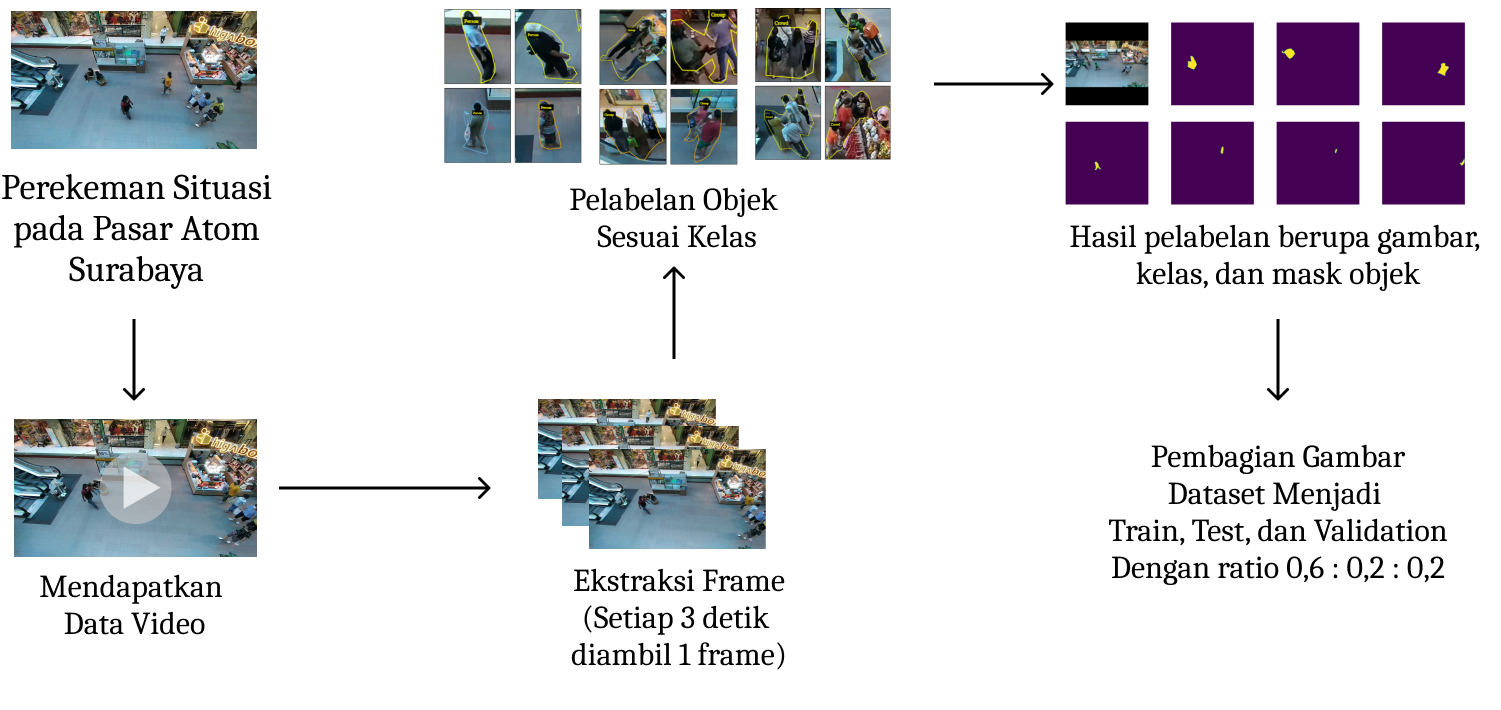
\includegraphics[width= 1.0\linewidth]{bab3/Pembentukan Dataset.png}
      \caption{Alur Pembentukan Dataset}
      \label{fig: base_method}
    \end{center}
  \end{figure}
  
  \subsection{Pengumpulan Data}
  Pada proses pengumpulan data, data mengenai aktivitas pembeli, penjual, dan petugas yang berada pada Pasar Atom
  akan diambil dalam bentuk video. Data tersebut akan diambil di berbagai lokasi pengamatan yang masih berada pada 
  kawasan Pasar Atom. Data video tersebut kemudian akan diubah menjadi gambar dengan cara mengekstrak satu gambar setiap
  tiga \textit{frame} pada video. Beberapa lokasi yang menjadi pengamatan ialah pintu masuk utama Pasar Atom, 
  lantai dua Pasar Atom, dan eskalator utama Pasar Atom. Pengumpulan data dilakukan menggunakan kamera 8 Mega Pixel dimana 
  tinggi kamera adalah 5 meter dan mempunyai sudut 30 derajat terhadap sumbu X. Data yang dikumpulkan merupakan data video
  berukuran 1920 x 1080 px.

  \begin{figure}[h!]
    \begin{center}
      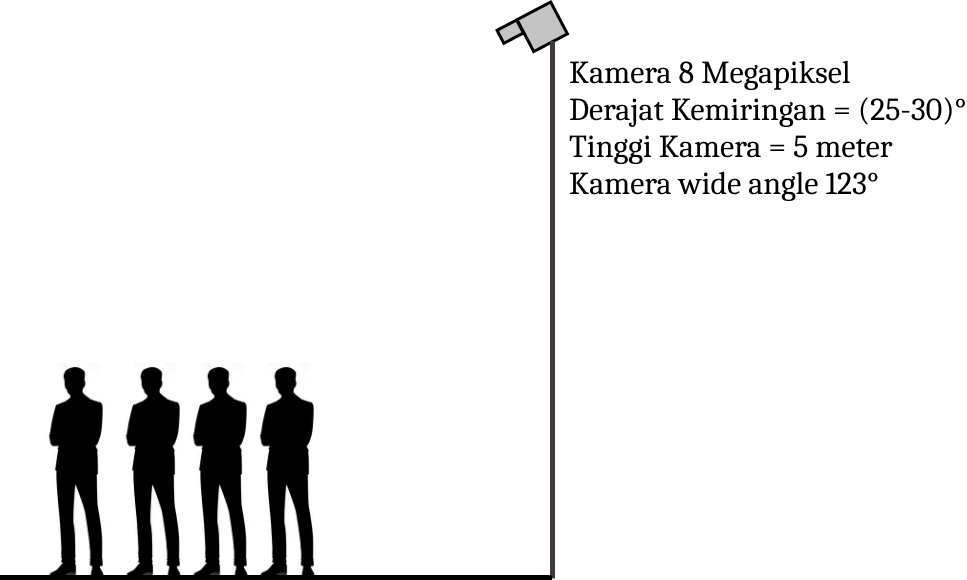
\includegraphics[width= 0.7\linewidth]{bab3/Konfigurasi tinggi kamera.png}
      \caption{Konfigurasi Pengambilan Gambar}
      \label{fig: base_method}
    \end{center}
  \end{figure}
  
  \subsection{Anotasi Data}
  Pada proses ini, data yang telah berupa gambar tersebut akan dianotasi menjadi tiga kelas sebagai berikut :
  
  \begin{itemize}
	  \item \textbf{Kelas \textit{Person}}
	  
	  Kelas \textit{Person} diberikan kepada objek orang yang tidak berada di dekat orang lain dalam jarak radius
	  satu meter.
  
	  \item \textbf{Kelas \textit{Group}}
	  
	  Kelas \textit{Group} diberikan kepada objek kelompok orang yang terdiri dari dua hingga tiga orang dalam
	  radius satu meter.
  
	  \item \textbf{Kelas \textit{Crowd}}
	  
	  Kelas \textit{Crowd} diberikan kepada objek kelompok orang yang terdiri dari empat atau lebih orang dalam
	  radius satu meter.
  \end{itemize}
  
  Proses anotasi dilakukan dengan \textit{software VGG Image Annotator (VIA)} \cite{dutta2019vgg}
  dimana pelabelan objek dilakukan dengan cara mensegmentasi objek dengan sebuah \textit{mask}. Proses anotasi menggunakan
  VIA adalah sebagai berikut.
  
  Kemudian hasil dari pelabelan tersebut akan diubah menjadi
  format \textit{JavaScript Object Annotation (.Json)} yang berisi mengenai koordinat segmentasi serta nama kelas 
  objek hasil anotasi. Hasil anotasi dan gambar yang telah diambil dari video inilah yang akan menjadi dataset
  penelitian mengenai deteksi kerumunan. Dataset kemudian akan dibagi menjadi \textit{train set}, \textit{test set},
  dan \textit{val set} dengan proporsi masing-masing secara berurutan 60\% \: 20\% \: 20\%. \textit{train set} akan
  digunakan untuk melatih algoritma pembelajaran mesin, \textit{val set} akan digunakan untuk mengukur performa model
  pada setiap iterasi, sedangkan \textit{test set} akan digunakan untuk memeriksa performa model akhir. \textit{Train set,
  val set,} dan \textit{Test set} memiliki gambar yang berbeda.
  
  \begin{figure}[h!]
	  \begin{center}
		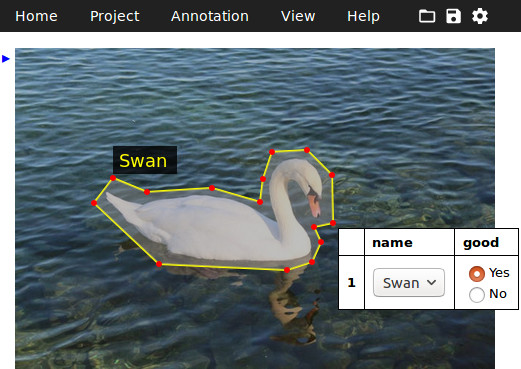
\includegraphics[width= 0.7\linewidth]{bab3/Demo Via.jpg}
		\caption{Software VIA \cite{dutta2019vgg}}
		\label{fig: VIA}
	  \end{center}
  \end{figure}
  
  \begin{figure}[h!]
	\begin{center}
	  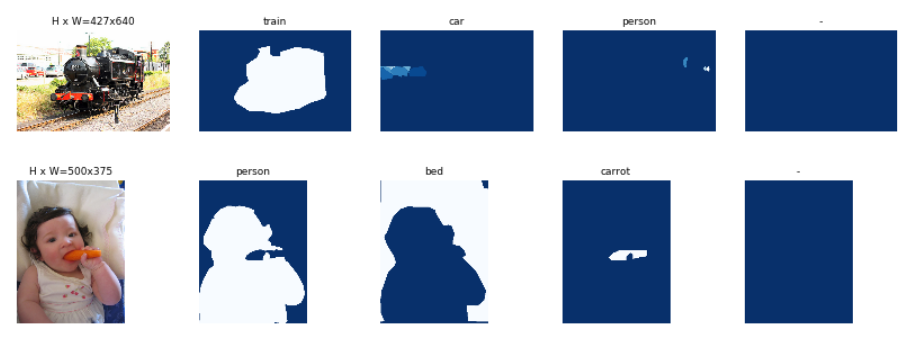
\includegraphics[width= 0.8\linewidth]{bab3/Contoh uji coba dataset.png}
	  \caption{Contoh Hasil Uji Coba Pembuatan Dataset \cite{matterport_maskrcnn_2017}}
	  \label{fig: Hasil Uji Coba}
	\end{center}
  \end{figure}
  
  
  \section{Data \textit{Preprocessing}}
  
  \begin{figure}[h!]
	  \begin{center}
		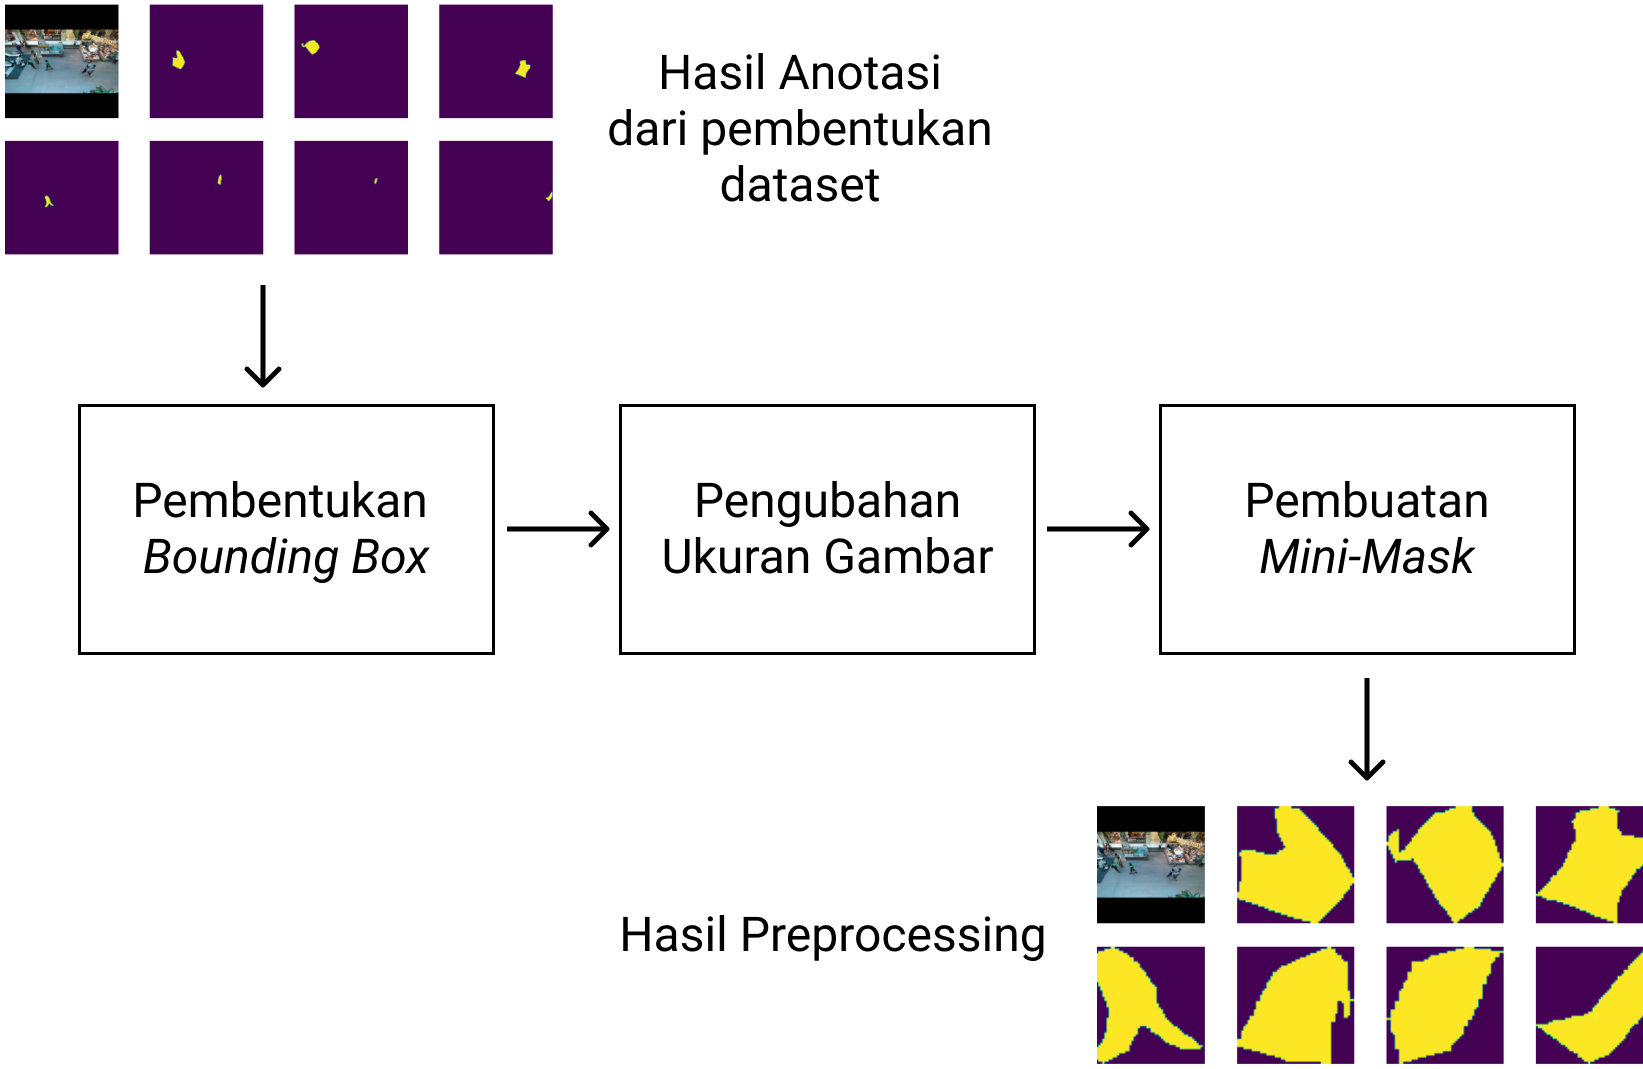
\includegraphics[width= 0.7\linewidth]{bab3/Preprocessing.png}
		\caption{Tahap \textit{Preprocessing}}
		\label{fig: Preprocessing}
	  \end{center}
  \end{figure}
  
  Pada tahap \textit{preprocessing} dataset yang telah dibentuk pada proses pembuatan dataset akan diolah terlebih 
  dahulu agar ukuran data menjadi lebih kecil dan
  proses ektraksi fitur maupun proses \textit{training} dapat dijalani secara lebih cepat dan tidak memerlukan 
  banyak sumber daya komputasi. Seperti yang telah tertera pada gambar \ref{fig: Preprocessing}, tahap \textit{preprocessing} dibagi menjadi 
  tiga yaitu pembuatan \textit{bounding box}, pengubahan ukuran gambar, dan pembuatan \textit{mini mask}.
  
  \subsection{Pembuatan \textit{Bounding Box}}
  Pada tahap ini,sbuah \textit{bounding box} akan dibentuk pada gambar-gambar yang telah memiliki objek anotasi.
  \textit{Bounding box} yang dibentuk mengikuti struktur panjang dan lebar segmentasi \textit{(mask)} yang telah 
  dibuat pada tahap pembuatan dataset. \textit{Bounding box} dibentuk mengikuti koordinat panjang dan lebar dari
  \textit{mask} agar jika gambar atau objek tersebut mengalami transformasi seperti pemutaran gambar, pengubahan
  ukuran gambar, dan pemotongan gambar, \textit{bounding box} dapat mengikuti koordinat transformasi dari 
  \textit{mask} pada objek yang telah melakukan transformasi. Proses ini tentunya lebih efektif daripada menghitung
  koordinat \textit{bounding box} setiap kali gambar melakukan transformasi.

  \subsection{Pengubahan Ukuran Gambar}
Pada tahap ini, setelah objek pada gambar diberikan \textit{bounding box} gambar akan diubah ukurannya menjadi
ukuran yang sama (\textit{uniform}) dimana pada penelitian ini, ditetapkan ukuran gambar adalah 1024 x 1024 karena
proses \textit{transfer learning} dari serta proses ekstraksi fitur mendukung ukuran tersebut. Jika gambar awal
tidak memiliki ukuran piksel 1024 pada kedua sisinya, maka sisi dengan nilai piksel terbesar akan diperpanjang 
hingga bernilai 1024, sedangkan sisi yang lain diperbesar mengikuti ratio awal. Jika salah satu sisi gambar telah
bernilai 1024, maka sisi yang lain akan ditambahkan piksel dengan nilai piksel 0 dimana gambar awal akhirnya
dipertahankan pada posisi tengah. Piksel bernilai 0 akan memberikan warna hitam pada gambar, sehingga pada proses 
ekstraksi fitur maupun deteksi citra, piksel bernilai 0 tidak memberikan dampak apapun dan hanya memakan sedikit 
daya komputasi.

\subsection{Pembentukan Mini Mask}
Pada tahap ini, setelah semua gambar memiliki nilai piksel yang sama, hasil segmentasi atau yang disebut
\textit{mask} pada data awal akan diekstrak dan mengalami perubahan ukuran. Pada awalnya \textit{mask} tiap objek
memiliki ukuran 1024 x 1024. Jika pada gambar tersebut memiliki banyak objek, misalnya sebagai contoh terdapat 10
objek, maka akan terdapat 11 gambar berukuran 1024 x 1024 piksel yang terdiri dari 10 gambar \textit{mask} dan 
1 gambar asli. Tentunya hal ini tidak efektif karena \textit{mask} tersebut akan memakan daya memori komputer 
saat melakukan proses \textit{training}, karena itu ukuran \textit{mask} akan diperkecil menjadi 56 x 56 piksel
dan hanya mengambil piksel \textit{mask}.

\section{Ekstraksi Fitur}

\begin{figure}[h!]
  \begin{center}
    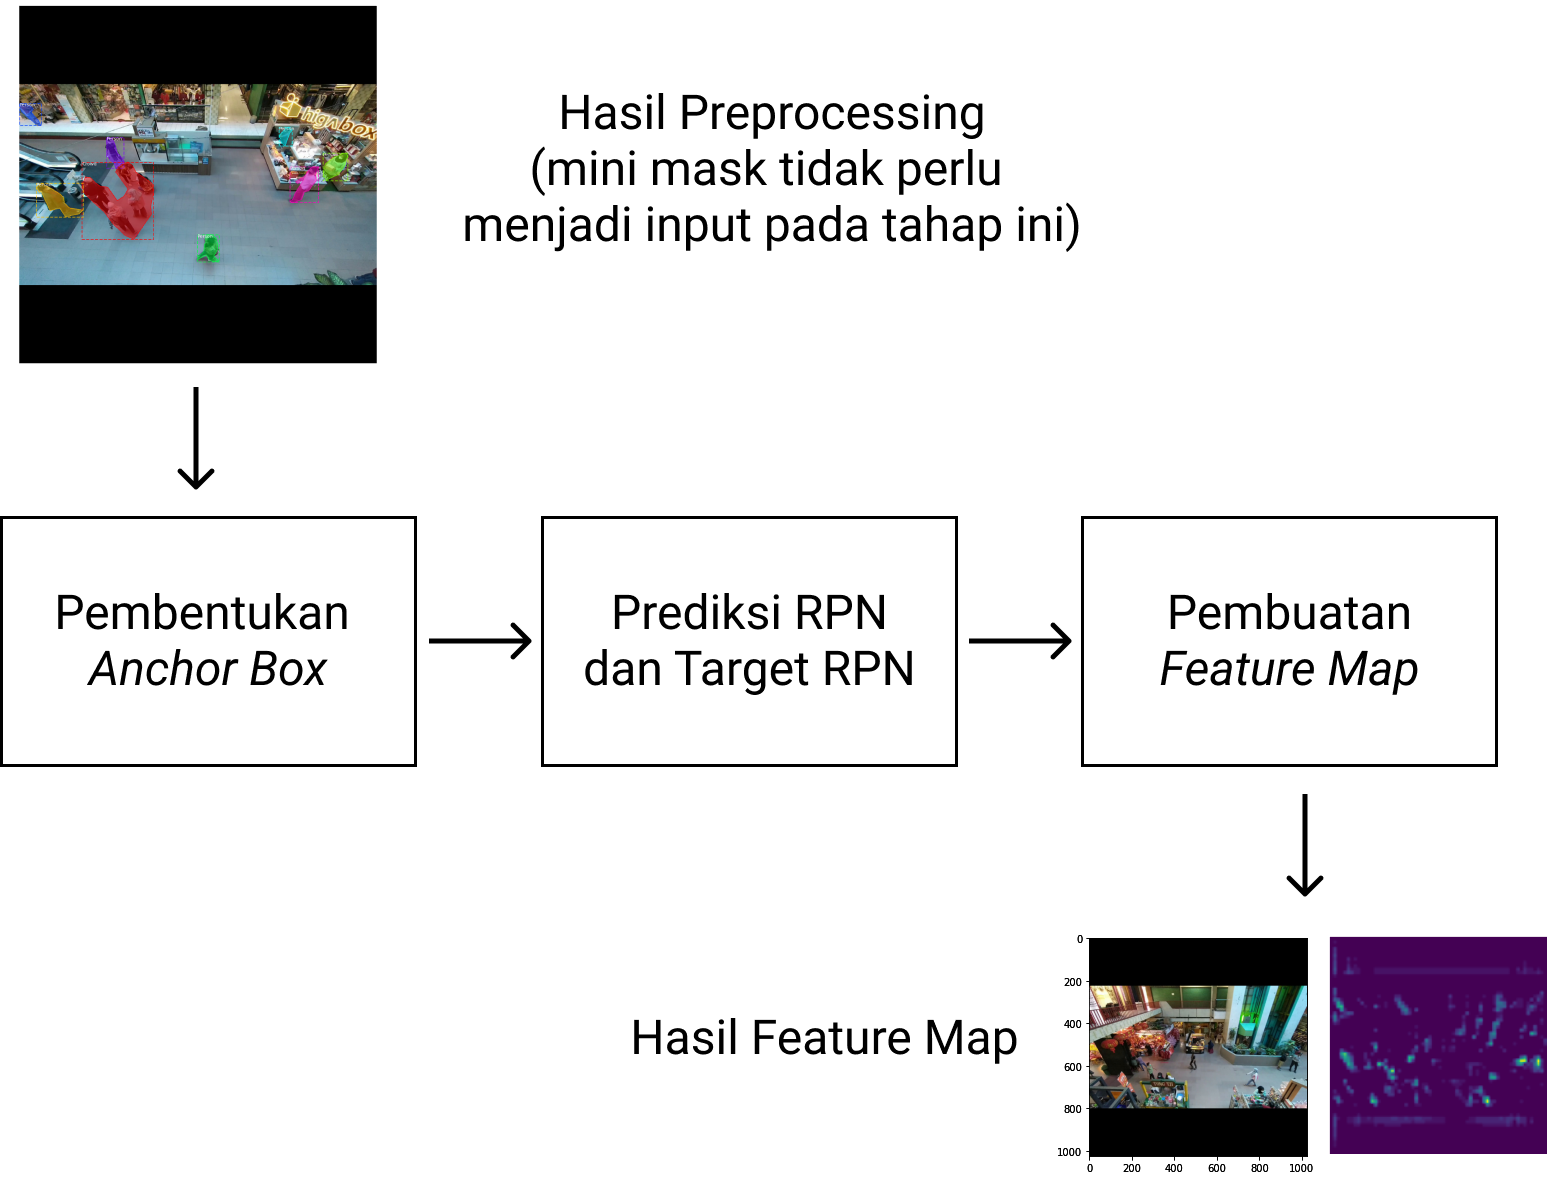
\includegraphics[width= 0.7\linewidth]{bab3/Ekstraksi Fitur.png}
    \caption{Proses Ektraksi Fitur}
    \label{fig: ekstraksi_fitur}
  \end{center}
\end{figure}

Proses ekstraksi fitur merupakan salah satu proses yang terpenting untuk memberikan data kepada algoritma deteksi
objek, dengan fitur-fitur yang diambil pada gambar, algoritma dapat menentukan lokasi serta kelas objek. Pada
penelitian ini, ekstraksi fitur menggunakan \textit{backbone} Resnet 101 yang memanfaatkan penggunaan 
\textit{anchor box}. Proses ekstraksi fitur yang perlu dilakukan pertama kali ialah membentuk \textit{anchor box},
kemudian berdasarkan \textit{anchor box} yang telah dibentuk, maka \textit{region proposal network} dapat dibangkitkan,
kemudian Resnet 101 akan digunakan untuk membuat sebuah \textit{feature map} berdasarkan \textit{region proposal
network} yang telah dibuat. \textit{Feature map} akan digunakan untuk mendeteksi lokasi, memberikan \textit{mask},
membangkitkan \textit{bounding box} dan mengklasifikasi kelas objek yang dideteksi.

\subsection{Pembuatan \textit{Anchor Box}}
Proses ekstraksi fitur yang pertama ialah pembuatan \textit{anchor box}, anchor box digunakan untuk mengetahui
lokasi \textit{bounding box} dan menjadi target dalam proses \textit{training} model dalam mendeteksi
\textit{regional proposal network (RPN)}. Terdapat 15 \textit{anchor box} yang dibentuk pada setiap iterasi.
Dapat dilihat pada gambar \ref{fig: Bentuk_Anchor_Box} bahwa \textit{anchor box} yang dibentuk memiliki lima
skala ukuran dan tiga jenis persegi empat yang mempunyai ukuran piksel yang berbeda. 15 belas \textit{anchor box}
tersebut akan disusun bertumpuk menyerupai piramid dan akan digeser setiap tiga piksel hingga semua piksel pada 
gambar telah terlingkupi oleh \textit{anchor box}. \textit{Anchor box} yang memiliki \textit{intersection over union}
atau irisan lebih dari sama dengan 70\% dengan \textit{bounding box} yang telah dibentuk pada tahap \textit{preprocessing}
dataset akan disimpan. Sedangkan \textit{anchor box} yang memiliki irisan kurang dari 70\% dengan \textit{bounding
box} yang telah dibuat akan dibuang dan tidak digunakan lagi. \textit{Anchor box} yang disimpan dinamakan 
target \textit{region proposal network} (RPN).

\begin{figure}[h!]
  \begin{center}
    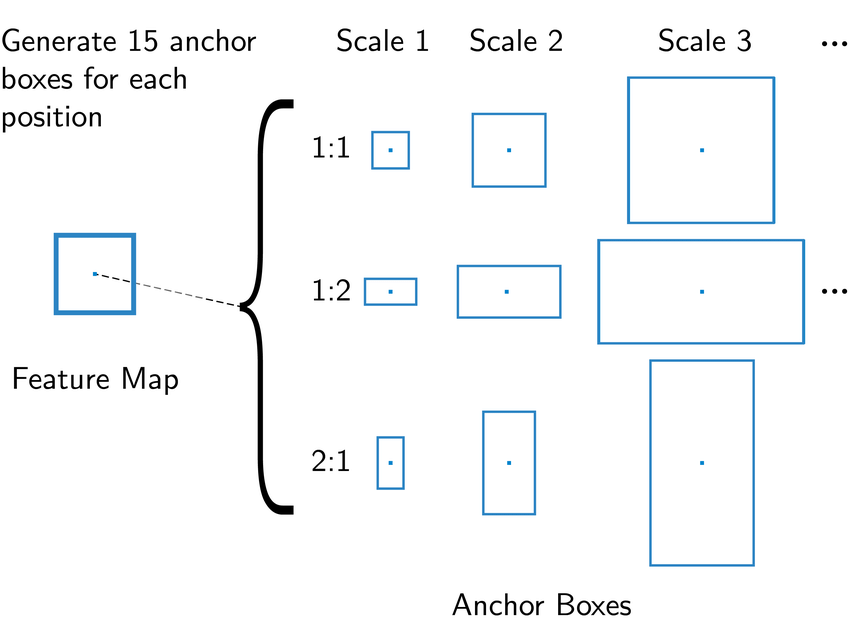
\includegraphics[width= 0.7\linewidth]{bab3/Anchor-Boxes-at-a-certain-position-in-the-feature-map.png}
    \caption{Bentuk \textit{Anchor Box} \cite{article_Anchor_Box}}
    \label{fig: Bentuk_Anchor_Box}
  \end{center}
\end{figure}

\subsection{Prediksi RPN}
Pada tahap sebelumnya, beberapa \textit{anchor box} yang mempunyai irisan dengan \textit{bounding box} asli telah
disimpan sebagai \textit{region of interest} positif . Target \textit{region proposal network} positif ini akan 
menjadi data untuk melatih model pada jaringan \textit{backbone}. Pada penelitian ini \textit{backbone} yang
digunakan ialah ResNet 101, sehingga jaringan \textit{Convolutional Neural Network} pada ResNet 101 akan dilatih
untuk dapat mendeteksi fitur yang ada pada \textit{regional proposal network}. Menggunakan beberapa iterasi maka
objek tersebut dapat dideteksi, kemudian suatu \textit{bounding box} hasil prediksi juga dibentuk, tentunya
\textit{bounding box} yang dibentuk terkadang dapat menimpa satu sama lain pada satu objek yang sama. Karena itu
penerapan algoritma \textit{non maximum supression} diperlukan agar \textit{bounding box} yang menimpa satu sama
lain dapat dihilangkan dan menjadi satu \textit{bounding box} yang optimal.

\subsection{Pembuatan \textit{Feature Map}}
Selain hasil berupa prediksi \textit{region proposal network}, \textit{backbone} ResNet 101 juga menghasilkan
sebuah \textit{feature map} yang merupakan hasil dari proses konvolusi dan pooling pada jaringan residual yang
digunakan. \textit{Feature map} ini akan digunakan sebagai data bagi \textit{fully connected layer} dan
\textit{layer konvolusi} untuk memprediksi kelas, \textit{bounding box}, dan \textit{mask}. Contoh hasil dari
\textit{feature map} dapat dilihat pada gambar \ref{fig: Feature Map example}.

\begin{figure}[h!]
  \begin{center}
    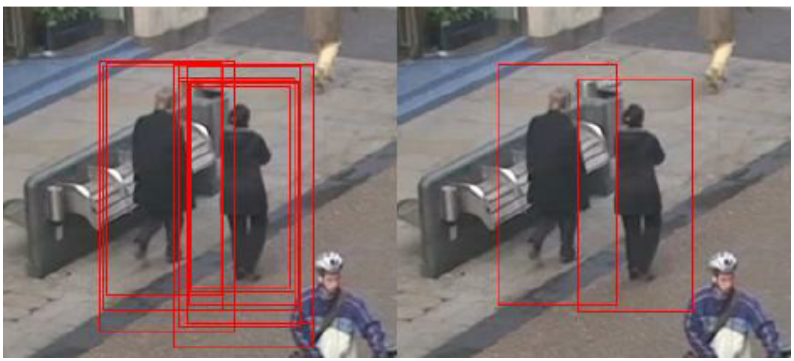
\includegraphics[width= 0.7\linewidth]{bab3/Non max suppression.png}
    \caption{Hasil \textit{non max supression} (kanan) \cite{Non_Max_Supression}}
    \label{fig: NMS}
  \end{center}
\end{figure}

\begin{figure}[h!]
  \begin{center}
    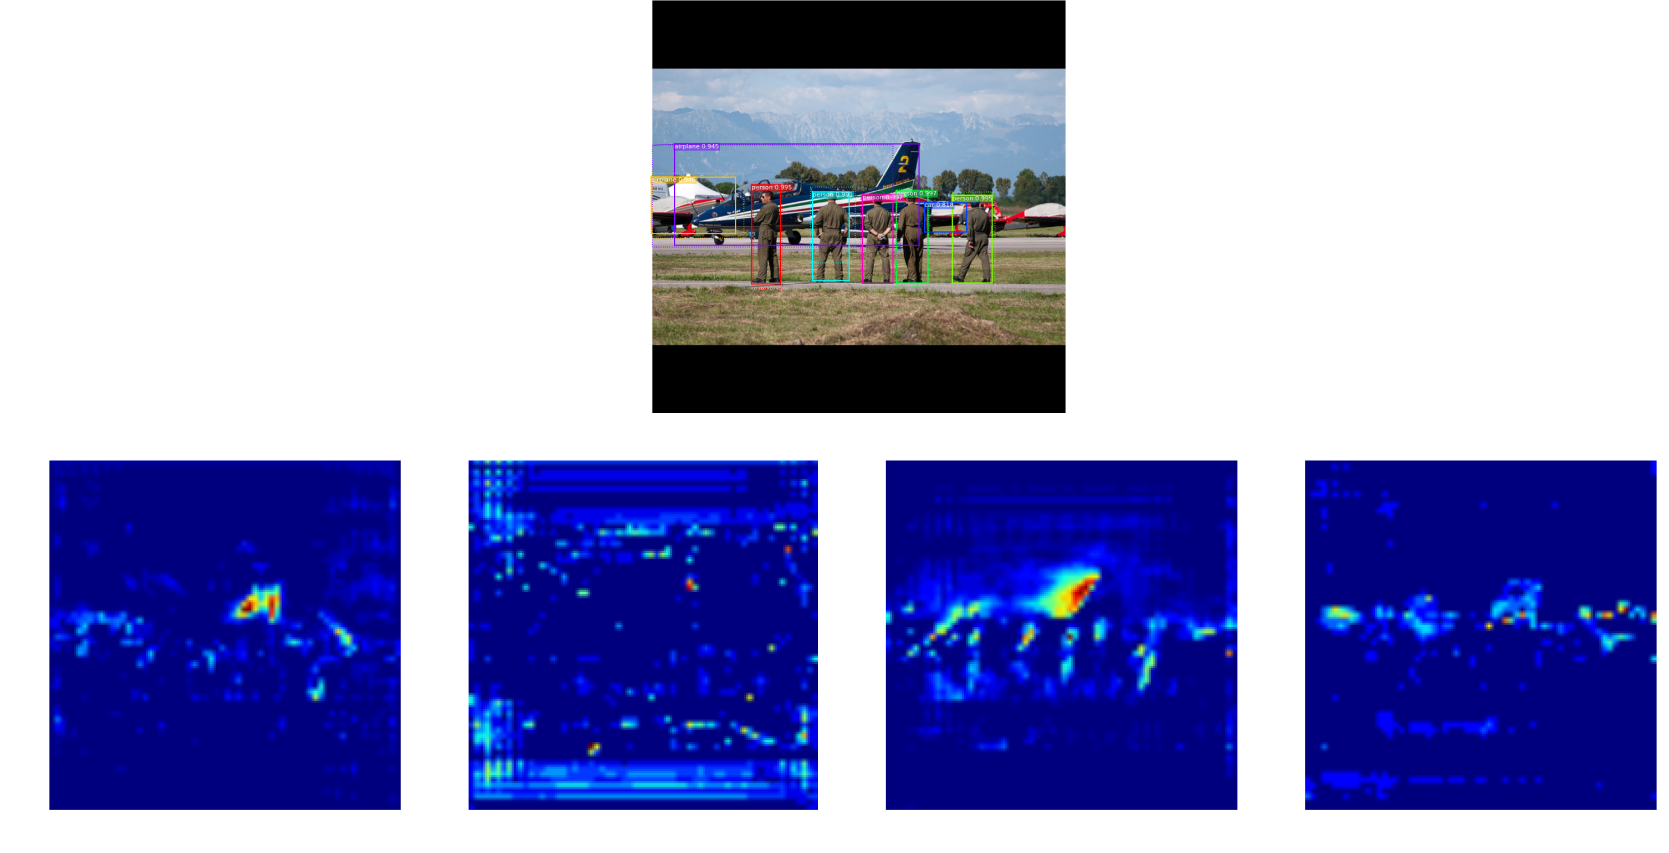
\includegraphics[width= 0.8\linewidth]{bab3/Contoh feature map.png}
    \caption{Contoh \textit{Feature map} pada \textit{layer} berbeda \cite{matterport_maskrcnn_2017}}
    \label{fig: Feature Map example}
  \end{center}
\end{figure}

\section{Proses Training}
Proses pembelajaran mesin sudah dilakukan pada tahap ekstraksi fitur, namun dalam mengklasifikasi
serta memberikan \textit{bounding box} yang tepat dari berbagai \textit{region proposal network} yang dibentuk
dari proses ekstraksi fitur, beberapa \textit{layer neural network} masih dibutuhkan dan perlu dilatih. 
Hasil keluaran dari \textit{layer convolutional neural network} dan \textit{fully connected layer} inilah yang
akan memberikan keluaran akhir dalam bentuk \textit{bounding box, mask}, dan kelas objek yang dideteksi.
Pada tahap ini sebuah \textit{fully connected layer} perlu dibentuk dalam mendeteksi kelas dan 
\textit{bounding box}. Selain itu, sebuah \textit{convolutional neural network} juga dibentuk untuk menghasilkan
\textit{mask} yang sesuai dengan objek. 

Pada tahap ini, beberapa \textit{hyperparameter} juga digunakan untuk mengatur
jalannya proses \textit{training}. \textit{Hyperparameter} yang daitur pada penelitian ini antara lain \textit{learning rate,epoch}
dan \textit{batch}. Pada penelitian ini pengaplikasian \textit{learning rate} dinamis juga akan diperkenalkan.
\textit{learning rate} dinamis digunakan dengan tujuan untuk mengurangi \textit{overfitting} dan mempercepat proses pembelajaran.
Pada \textit{epoch} 1 hingga 20, \textit{learning rate} yang digunakan adalah 0.01, pada \textit{epoch} 21 hingga
60, \textit{learning rate} yang digunakan adalah 0.005, sedangkan pada \textit{epoch} 61 hingga 150, 
\textit{learning rate} yang digunakan adalah 0.001 yang merupakan nilai terkecil yang digunakan pada penelitian
ini, detail \textit{learning rate} yang digunakan dapat dilihat pada tabel \ref{tab:lr_config}. Sedangkan
detail mengenai \textit{hyperparameter} dapat dilihat pada tabel \ref{tab:MaskRCCN_config}.

\begin{table}
  \caption{Konfigurasi pada proses \textit{training}}
  \label{tab:MaskRCCN_config}
  \centering
  \begin{tabular}{ | l | l | }
    \hline
    \textbf{Jenis Konfigurasi} & \textbf{Keterangan} \\ \hline
    \textit{batch}             & 1                   \\ \hline
    \textit{learning rates}    & dinamis dari 0.001 hingga 0.01                \\ \hline
    \textit{epoch}             & 150                   \\ \hline
  \end{tabular}
\end{table}

\begin{table}
  \caption{\textit{learning rate} dinamis}
  \label{tab:lr_config}
  \centering
  \begin{tabular}{ | l | l | }
    \hline
    \textbf{Epoch} & \textbf{Learning Rate} \\ \hline
    \textit{1 - 20}             & 0.01                   \\ \hline
    \textit{21 - 60}    & 0.005                \\ \hline
    \textit{61 - 150}             & 0.001                  \\ \hline
  \end{tabular}
\end{table}

\section{Proses Pengujian}
Proses pengujian model dalam penelitian ini dibagi menjadi 2 bagian, bagian yang pertama dilakukan pada saat 
model selesai melakukan proses \textit{training} namun masih memiliki iterasi \textit{epoch} yang belum selesai. 
Proses ini bernama validasi, dimana akurasi dari uji coba mode pada \textit{val set} akan dilakukan. 
Proses ini sangat vital karena dengan validasi kita dapat mengetahui apakah model 
kita mengalami \textit{overfitting} dimana performa model dalam mendeteksi objek di gambar baru dirasa kurang
maupun \textit{underfitting} dimana model tidak menunjukkan kemajuan dalam mendeteksi objek pada gambar. 
Salah satu ciri yang paling mudah yang 
menandakan kemungkinan terjadinya \textit{overfitting} adalah ketika besaran \textit{training loss} suatu model 
menjadi semakin kecil, namun besaran \textit{validation loss}-nya malah semakin besar di setiap iterasi. 
Sedangkan \textit{underfitting} terjadi ketika baik \textit{training loss} maupun \textit{validation loss} 
memiliki nilai yang terlalu besar. Selain itu pada proses validasi ini, data yang digunakan adalah data yang 
sama sekali baru dan tidak digunakan selama proses \textit{training} guna menghindari kemungkinan terjadinya 
bias yang biasa terjadi apabila suatu model diuji pada data yang sama yang digunakan pada saat proses 
\textit{training}. Berdasarkan data pada proses validasi, algoritma \textit{optimizer} akan memutuskan untuk 
merubah \textit{weight} dalam pada \textit{neural network} sehingga semakin mendekati titk akurasi tertingginya.

Bagian selanjutnya dari proses pengujian adalah melakukan \textit{test}. Sama seperti pada waktu proses validasi, 
dataset yang digunakan juga sama sekali berbeda dengan data yang digunakan pada waktu \textit{training} maupun 
pada waktu \textit{validasi}. Dari proses ini, dapat diambil kesimpulan apakah suatu model tersebut dapat 
dilakukan perbaikan lagi denga cara \textit{re-training} dan merubah beberapa parameter maupun konfigurasi 
yang sudah diatur pada saat proses \textit{training}, ataukah model tersebut dirasa sudah cukup baik dan akan 
melanjutkan ke proses berikutnya. Adapun beberapa metriks yang dapat diketahui dari proses 
\textit{training} yaitu metriks \textit{train accuracy, loss, val-accuracy} dan \textit{val-loss}.
\textit{loss function} yang diberikan merupakan jumlah segala \textit{loss} yang terjadi pada tiap tahapan
proses pada algoritma Mask R-CNN yang ditetapkan. Persamaan total \textit{loss} dapat dilihat pada persamaan
\ref{eq :loss}. Sedangkan persamaan total \textit{mask loss} dapat dilihat pada persamaan \ref{eq :mask loss}. Untuk
persamaan mengenai \textit{loss} yang terjadi pada kelas serta \textit{bounding box}, dapat dilihat pada
persamaan \ref{eq:other Loss}.

\begin{equation}
  \label{eq :loss}
  \mathcal{L} = \mathcal{L}_\text{cls} + \mathcal{L}_\text{box} + \mathcal{L}_\text{mask}
\end{equation}

\begin{equation}
  \label{eq:other Loss}
  \mathcal{L}_\text{fr} = \mathcal{L}_\text{cls} + \mathcal{L}_\text{box}
\end{equation}

\begin{equation}
  \mathcal{L}_\text{fr}(\{p_i\}, \{t_i\}) = \frac{1}{N_\text{cls}} \sum_i \mathcal{L}_\text{cls} (p_i, p^*_i) + \frac{\lambda}{N_\text{box}} \sum_i p^*_i \cdot L_1^\text{smooth}(t_i - t^*_i)
\end{equation}

\begin{equation}
  \label{eq :cls_loss}
  \mathcal{L}_\text{cls} (p_i, p^*_i) = - p^*_i \log p_i - (1 - p^*_i) \log (1 - p_i)
\end{equation}

\begin{equation}
  \label{eq :bbox loss}
  \mathcal{L}_\text{box} = \frac{\lambda}{N_\text{box}} \sum_i p^*_i \cdot L_1^\text{smooth}(t_i - t^*_i)
\end{equation}

\begin{equation}
  \label{eq :mask loss}
  \mathcal{L}_\text{mask} = - \frac{1}{m^2} \sum_{1 \leq i, j \leq m} \big[ y_{ij} \log \hat{y}^k_{ij} + (1-y_{ij}) \log (1- \hat{y}^k_{ij}) \big]
\end{equation}

\section{Analisa Performa}
Setelah melakukan proses pengujian, langkah berikutnya adalah melakukan analisa perforrma pada model yang 
sudah dibuat. Hal ini untuk mengetahui bagaimana kira - kira performa model pada saat sudah diimplementasi. 
Untuk analisa performa, model akan diuji pada dataset \textit{test}, dimana model tersebut akan mendeteksi
gambar-gambar yang belum pernah dilihat sebelumnya. Untuk mengetahui performa model, 
analisanya akan menggunakan beberapa metode seperti \textit{confusion matrix} untuk mendapatkan
pengelompokkan berdasarkan data menjadi \textit{True Positive} (TP), \textit{False Positive} (FP), 
\textit{True Negative} (TN), dan \textit{False Negative} (FN) dalam proses deteksi.
Selain itu, penelitian ini juga akan menggunakan rumus - rumus seperti \textit{Recall, Precision} dan 
\textit{Accuracy} dalam mengetahui performa model.







	\cleardoublepage
	\chapter{PENGUJIAN}
\label{sec:chap4_pengujian}
\vspace{1ex}

\section*{}
Pada penelitian ini dipaparkan hasil dari proses yang dipaparkan pada bab 3 serta analisa yang dilakukan sesuai 
dengan desain sistem yang sudah dirancang pada bab sebelumnya. Pembahasan hasil penelitian dilakukan
dengan beberapa bagian seperti berikut :

\begin{itemize}[nolistsep]
    \item Hasil dari Pembuatan Dataset
    \item Hasil \textit{Preprocessing} Data.
    \item Hasil Ekstraksi Fitur.
    \item Hasil Pembelajaran Mesin Mask R-CNN.
    \item Hasil Model Akhir Mask R-CNN.
\end{itemize}

Bagian pertama ialah membahas mengenai hasil dari pembuatan dataset, pada bagian ini akan dijelaskan mengenai
jumlah anotasi objek yang dibentuk. Kemudian pada bagian \textit{preprocessing}, akan dijelaskan hasil mengenai
pembuatan \textit{bounding box}, dan \textit{mini mask}. Kemudian pada bagian ekstraksi fitur dan hasil pembelajaran
mesin Mask R-CNN akan membahas mengenai \textit{pipeline} dari algoritma \textit{Mask R-CNN} secara kesuluruhan.
Kemudian terakhir pada bagian hasil model akhir Mask R-CNN akan dijelaskan mengenai 

\section{Hasil Pembuatan Dataset}
Pengambilan data video dilakukan di Pasar Atom pada bulan Januari 2022 dimana total video yang dikumpulkan adalah 24 menit
dan terdiri dari 6 lokasi. Pengambilan data dilakukan pada jam 1 hingga 2 siang. Setelah pengambilan video dilakukan,
1 frame setiap 90 frame pada video diekstrak sehingga menghasilkan 730 gambar. Gambar-gambar ini kemudian dibagi
menjadi tiga set (\textit{train set, test set} dan \textit{val set}) dengan perbandingan 0.6 : 0.2 : 0.2.
\textit{Train set} memiliki total gambar 436 gambar, \textit{test set} memiliki total 146 gambar, dan sama
seperti \textit{test set}, val set juga memiliki 146 gambar. Kemudian pada setiap gambar tersebut, objek manusia
dibedakan menjadi tiga kelompok atau kelas. Seperti yang sudah dijelaskan pada bab sebelumnya, kelas tersebut ialah

\begin{itemize}
    \item Kelas \textit{Person}, dimana objek manusia tersebut berada sendirian pada radius satu meter dapat dilihat
    pada gambar \ref{fig: Kelas Person}.
    \item Kelas \textit{Group}, dimana terdapat dua hingga tiga orang yang berada pada radius satu meter dapat dilihat
    pada gambar \ref{fig: Kelas Group}.
    \item Kelas \textit{Crowd}, dimana terdapat empat orang atau lebih yang berada berdekatan pada jarak radius
        satu meter dapat dilihat pada gambar \ref{fig: Kelas Crowd}.
\end{itemize}

\begin{figure}[h!]
    \begin{center}
      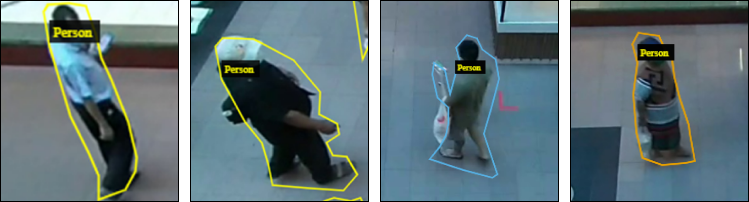
\includegraphics[width= 0.8\linewidth]{bab4/Person_class_2.png}
      \caption{Contoh Kelas \textit{Person}}
      \label{fig: Kelas Person}
    \end{center}
\end{figure}

\begin{figure}[h!]
    \begin{center}
      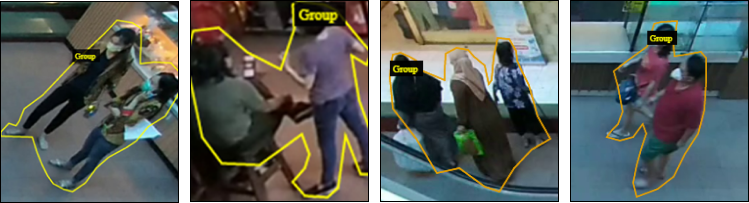
\includegraphics[width= 0.8\linewidth]{bab4/Group_class_2.png}
      \caption{Contoh Kelas \textit{Group}}
      \label{fig: Kelas Group}
    \end{center}
\end{figure}

\begin{figure}[h!]
    \begin{center}
      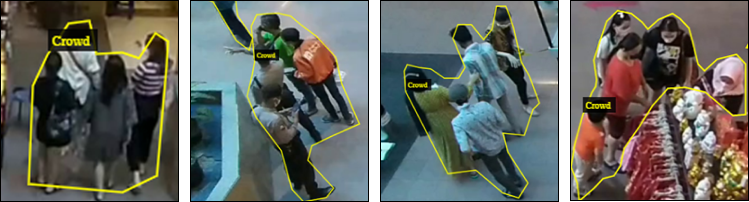
\includegraphics[width= 0.8\linewidth]{bab4/Crowd_class_2.png}
      \caption{Contoh Kelas \textit{Crowd}}
      \label{fig: Kelas Crowd}
    \end{center}
\end{figure}

Total objek yang dianotasi pada seluruh 730 gambar adalah 4.980 objek yang terdiri dari 3.382 objek kelas 
\textit{person}, 1.350 kelas \textit{group}, dan 248 kelas \textit{crowd}. Sedangkan jika dibagi pada tiap set,
\textit{Train set} memiliki 2.054 objek kelas \textit{person}, 732 objek kelas \textit{group}, dan 159 objek
kelas \textit{crowd}. \textit{Test set} memiliki 687 objek kelas \textit{person}, 321 objek kelas \textit{group},
dan 40 objek kelas \textit{crowd}. Sedangkan pada \textit{val set} memiliki 641 objek kelas \textit{person}, 
297 objek kelas \textit{group}, dan 49 objek kelas \textit{crowd}. Dapat dikatakan bahwa dataset ini merupakan
dataset yang tidak seimbang (\textit{imbalance dataset}) namun dalam kondisi Covid-19, objek kerumunan memang lebih
jarang ditemukan dibandingkan objek \textit{person} atau orang yang menjaga jarak satu sama lain. Tentunya hal ini
juga dapat digunakan untuk melihat perilaku para pengunjung, penjual, maupun petugas saat kondisi Covid-19. Dataset
ini juga dapat membantu penelitian lain dalam mengembangkan suatu program deteksi kerumunan terutama dalam pusat 
perbelanjaan.

\begin{table}[h]
    \caption{Detail Jumlah Objek Anotasi}
    \label{tab:specs_collab}
    \centering
    \begin{tabular}{|l|l|l|l|}
        \hline
        \textbf{Set}                    & Kelas \textit{Person} & Kelas \textit{Group} & Kelas \textit{Crowd}   \\ \hline
        \textit{\textbf{Train Set}}      & 2.054 & 732 & 159        \\ \hline
        \textit{\textbf{Test Set}}     & 687 & 321 & 40             \\ \hline
        \textit{\textbf{Val Set}}       & 641 & 297 & 49            \\ \hline
    \end{tabular}
\end{table}

\begin{figure}[h!]
    \begin{center}
      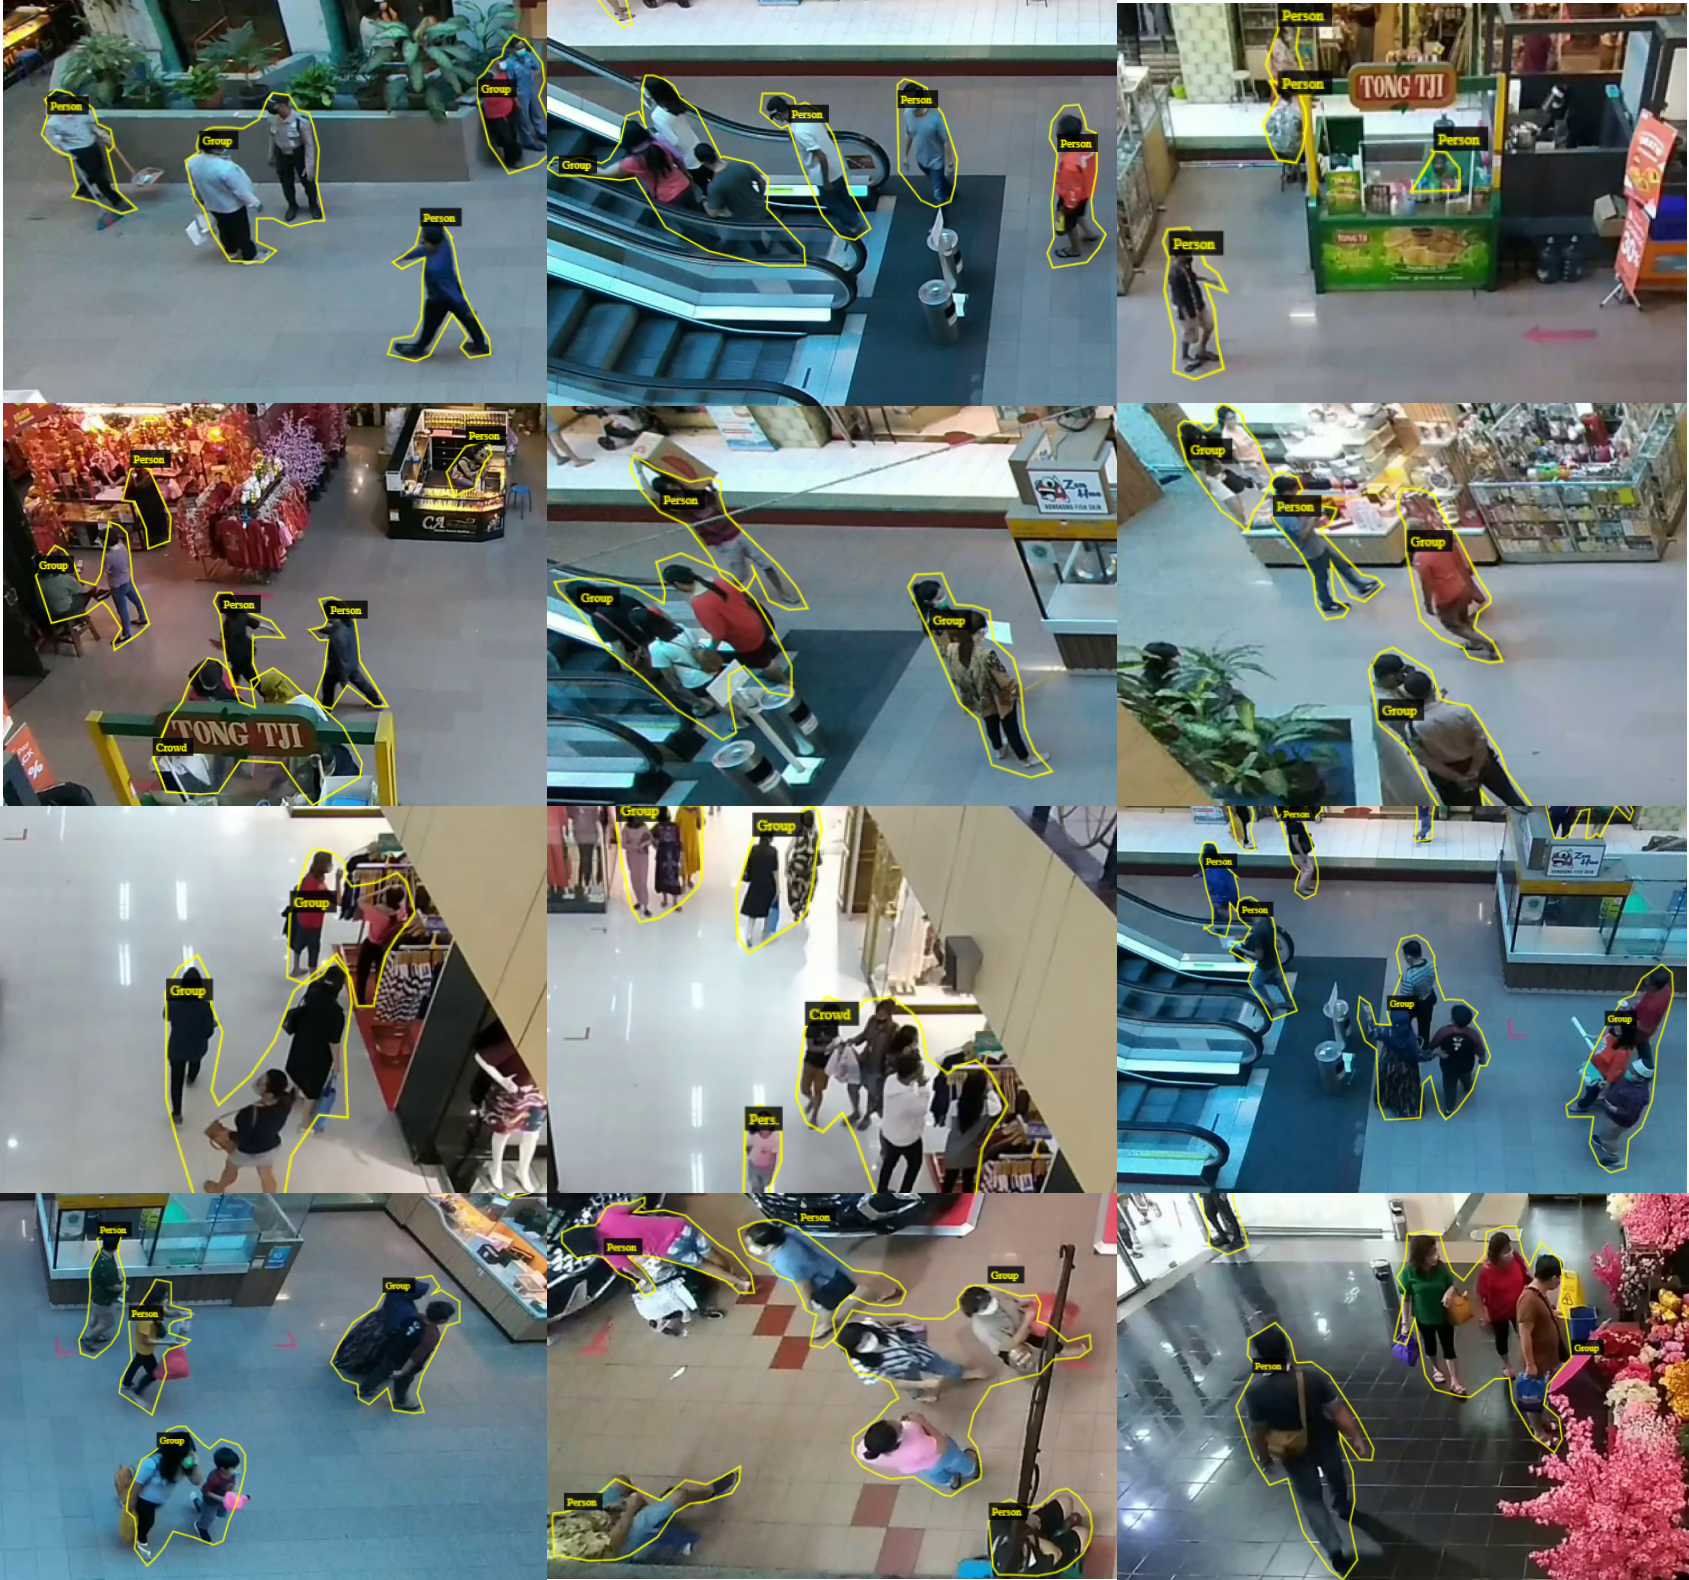
\includegraphics[width= 0.8\linewidth]{bab4/Dataset.png}
      \caption{Contoh Beberapa Hasil Dataset}
      \label{fig: Dataset}
    \end{center}
\end{figure}

\section{Hasil \textit{Preprocessing} Data}
Pada bagian ini, hasil mengenai \textit{preprocessing data pipeline} pada dataset yang telah dibentuk akan dijelaskan
secara lebih mendalam. 

\subsection{Hasil Pembuatan \textit{Bounding Box}}
Seperti yang telah dijelaskan sebelumnya pada bab metodologi, pembuatan \textit{bounding box} dilakukan dengan
mengikuti ukuran dari \textit{mask}. Jumlah \textit{bounding box} pada tahap ini mempunyai nilai yang sama dengan
jumlah objek pada dataset yaitu 4.970 objek.

\begin{figure}[h!]
  \begin{center}
    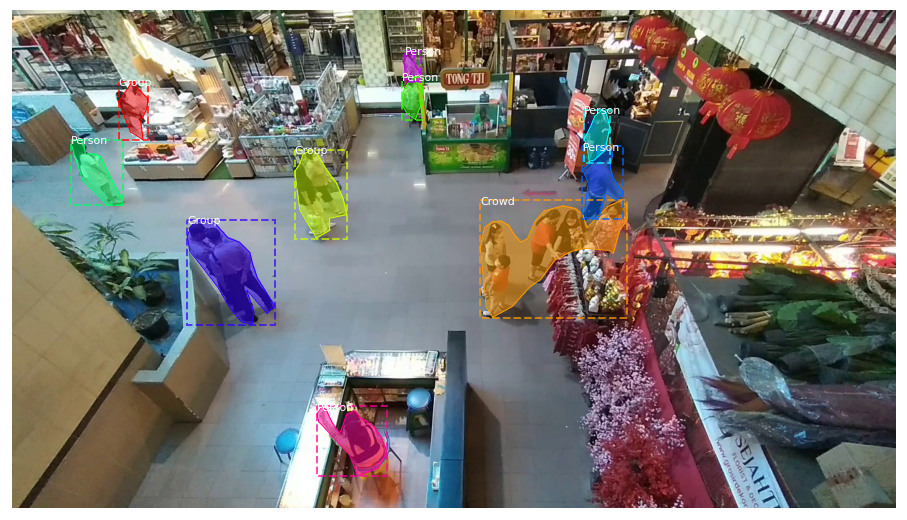
\includegraphics[width= 0.8\linewidth]{bab4/Contoh Bounding Box.png}
    \caption{Contoh Hasil Pembuatan \textit{Bounding Box}}
    \label{fig: Contoh Bounding Box}
  \end{center}
\end{figure}

\subsection{Hasil Pengubahan Ukuran Gambar}
Setelah koordinat \textit{bounding box} didapatkan dan \textit{bounding box} dapat dibentuk, maka ukuran gambar akan
disamakan sesuai dengan input pada model dimana pada penelitian ini ialah 1024 x 1024 piksel. Ukuran gambar yang awalnya
berukuran 1920 x 1080 dirubah menjadi 1024 x 1024 dengan cara memperkecil ukuran gambar dan memberikan piksel
hitam pada bagian atas dan bawah gambar. Hasil dari \textit{preprocess} ini dapat dilihat pada gambar 
\ref{fig: Contoh Resize Image}. Dimensi gambar pun berubah menjadi 1024 x 1024 x 3. Pada penelitian  ini
fitur warna tetap digunakan sebagai fitur, walaupun mungkin dalam kenyataannya, dimensi warna ini dapat dirubah
menjadi satu jenis saja.

\begin{figure}[h!]
  \begin{center}
    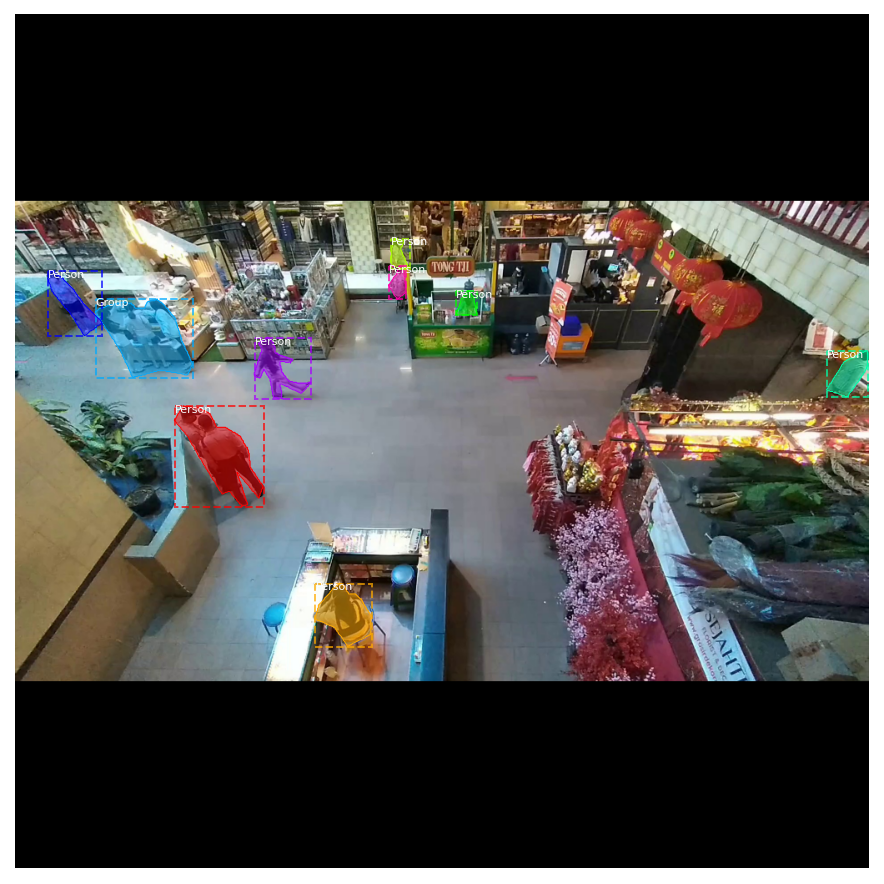
\includegraphics[width= 0.65\linewidth]{bab4/Resize Image.png}
    \caption{Contoh Hasil \textit{Resizing} Image}
    \label{fig: Contoh Resize Image}
  \end{center}
\end{figure}


\subsection{Hasil Pembuatan \textit{Mini Mask}}
Setelah gambar-gambar dataset mempunyai ukuran yang sama dan sesuai dengan input dari model, maka hal selanjutnya
yang perlu dilakukan ialah pembentukan \textit{mini mask}. Sebelumnya, \textit{mask} yang terbentuk pada dataset
juga mempunyai ukuran yang sama pada gambar, tentunya hal ini tidak efektif karena \textit{mask} tersbeut dibedakan
sesuai objeknya dan mempunyai banyak nilai null. Karena itu, bentuk \textit{mask} diubah menjadi ukuran 56 x 56 piksel.

\begin{figure}[h!]
  \begin{center}
    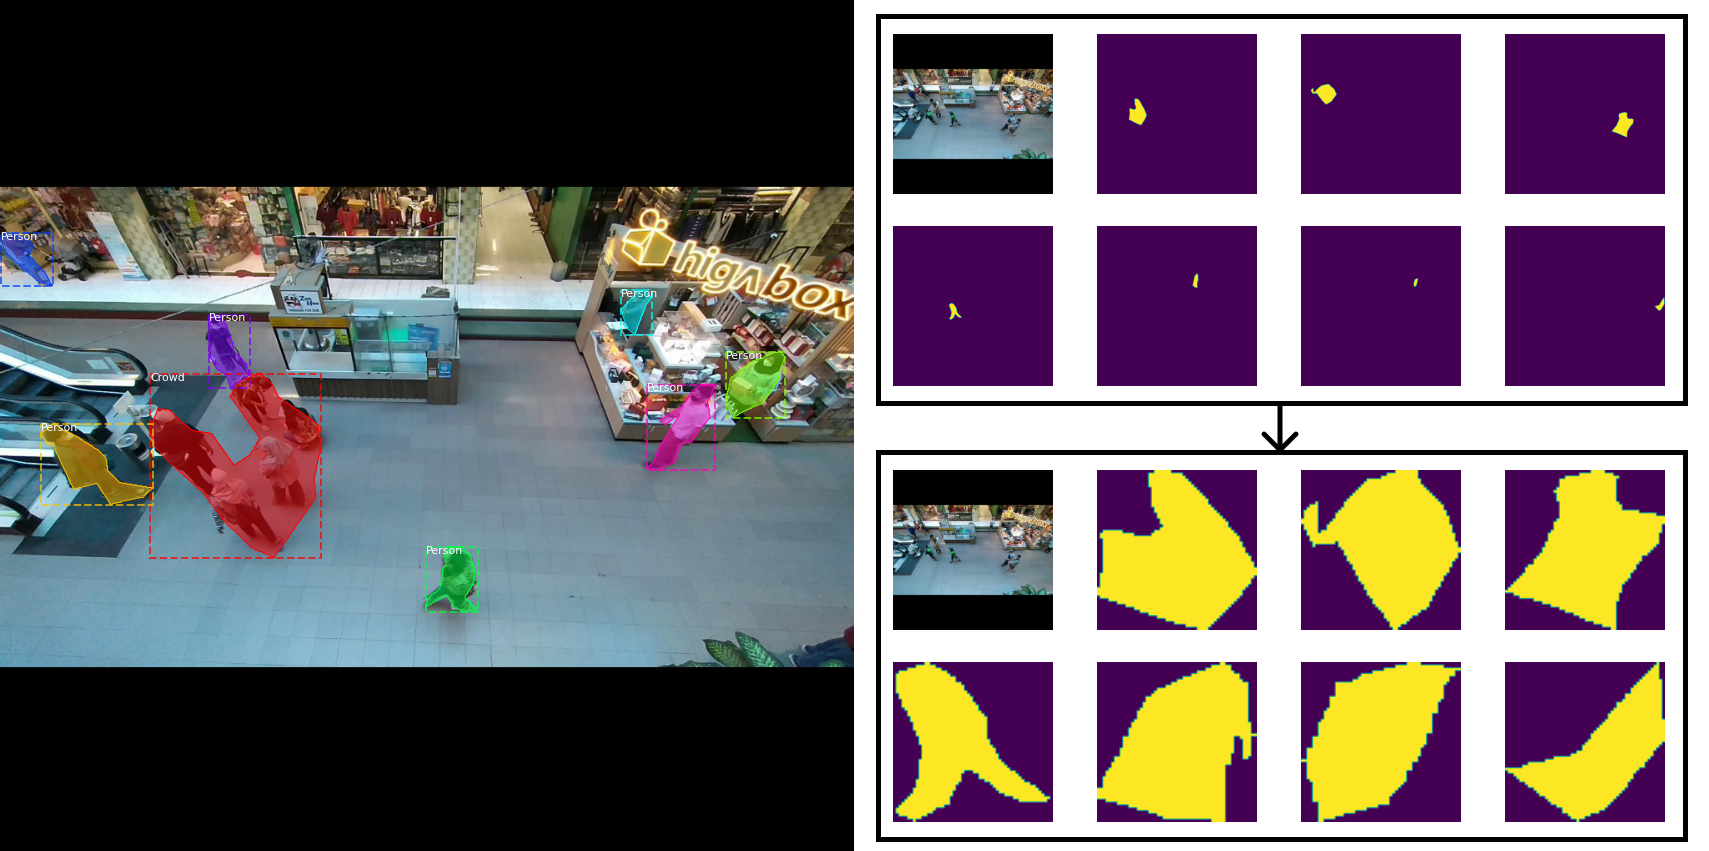
\includegraphics[width= 0.8\linewidth]{bab4/Mini Mask.png}
    \caption{Contoh Hasil Pembuatan \textit{Mini Mask}}
    \label{fig: Contoh Mini Mask}
  \end{center}
\end{figure}

\section{Hasil \textit{Feature Extraction}}
Pada bagian ini, hasil mengenai \textit{feature extraction pipeline} pada dataset yang telah di-\textit{preprocess}
akan dijelaskan secara lebih mendalam. Proses \textit{feature extraction} yang dilakukan pada tahap ini sudah
menggunakan algoritma Mask-RCNN. Namun hasil yang dikemukakan pada bagian ini adalah hasil \textit{feature map}.
Sedangkan hasil mengenai proses Mask R-CNN yang memberikan klasifikasi kelas, \textit{bounding box}, dan membangkitkan
\textit{mask}.

\begin{figure}[h!]
    \begin{center}
      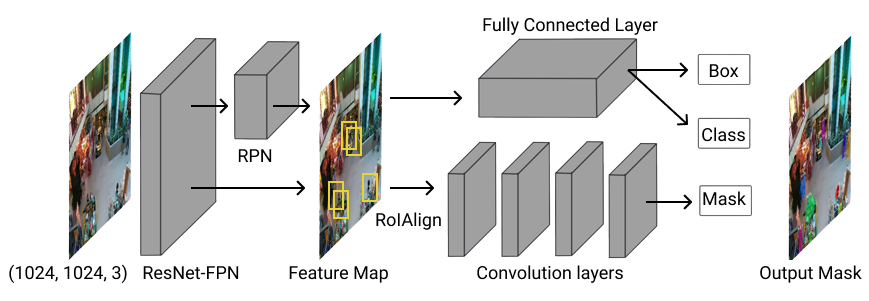
\includegraphics[width= 0.8\linewidth]{bab4/Metodologi_Training_2.png}
      \caption{Arsitektur Mask R-CNN yang diaplikasikan}
      \label{fig: Crowd Mask RCNN Archi}
    \end{center}
\end{figure}

Sesuai dengan proses algoritma Mask R-CNN yang diilustrasikan pada gambar \ref{fig: Crowd Mask RCNN Archi}
Proses Mask R-CNN dimulai dengat ekstraksi fitur pada jaringan \textit{backbone} dimana pada penelitian ini
\textit{backbone} yang digunakan ialah ResNet 101. Kemudian hasil dari ResNet akan menghasilkan prediksi
RPN \textit{Regional Proposal Network} serta \textit{feature map} yang merupakan hasil dari konvolusi dan
\textit{pooling} pada jaringan ResNet, kemudian pada \textit{feature map} tersebut akan diproses oleh
\textit{fully connected layer} untuk melakukan prediksi mengenai \textit{bounding box} pada objek serta
kelas daripada objek tersebut. Selain itu \textit{convolution layer} akan menggunakan fitur-fitur pada 
\textit{feature map} untuk membentuk \textit{mask} dari objek. Hasil \textit{training} dari pemprosesan
oleh \textit{Fully Connected Layer} dan \textit{Convolution Layer} akan dijelaskan pada subbab berikutnya.

\subsection{Hasil \textit{Pembuatan Anchor Box}}
Bagian pertama pada proses \textit{feature extraction} adalah membuat \textit{anchor box} yang akan digunakan
untuk target RPN. Untuk penentuan \textit{anchor box} yang akan menjadi target RPN, maka digunakan metriks IoU
\textit{Intersect over Union}, jika \textit{bounding box ground} atau \textit{bounding box} asli memiliki IoU lebih
dari sama dengan 0.7 dengan \textit{anchor box}, maka \textit{anchor box} tersebut digunakan sebagai target RPN.
Hasil dari pembuatan \textit{anchor box} ditunjukkan pada gambar \ref{fig: Anchor Box}. Sedangkan contoh 
\textit{anchor box} yang digunakan sebagai target RPN dapat dilihat pada gambar \ref{fig: Anchor Box Positive}.
Untuk menunjukkan adanya perbedaan mengenai \textit{anchor box} yang digunakan sebagai target dan dengan
yang tidak maka hasil \textit{anchor box} yang tidak digunakan pada proses melatih jaringan \textit{backbone} dalam
memprediksi RPN juga ditampilkan dan dapat dilihat pada \ref{fig: Anchor Box Negative}.

\begin{figure}[h!]
  \begin{center}
    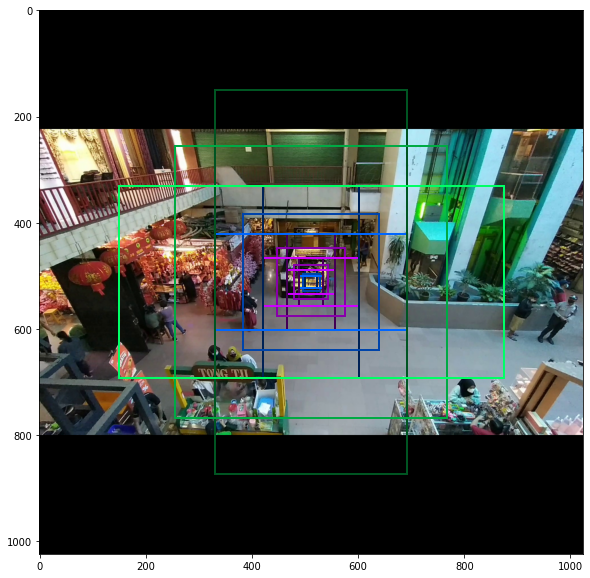
\includegraphics[width= 0.55\linewidth]{bab4/Anchor Box.png}
    \caption{Hasil \textit{Anchor Box} yang Dihasilkan}
    \label{fig: Anchor Box}
  \end{center}
\end{figure}

\begin{figure}[h!]
  \begin{center}
    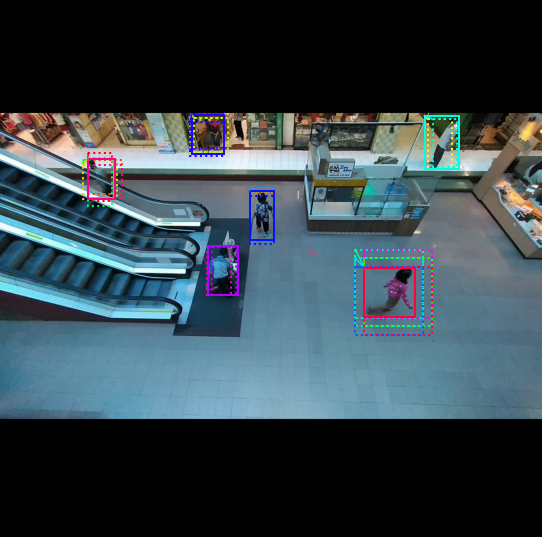
\includegraphics[width= 0.5\linewidth]{bab4/Anchor Box Positive.png}
    \caption{Contoh Hasil \textit{Anchor Box} yang Menjadi Target RPN}
    \label{fig: Anchor Box Positive}
  \end{center}
\end{figure}

\begin{figure}[h!]
  \begin{center}
    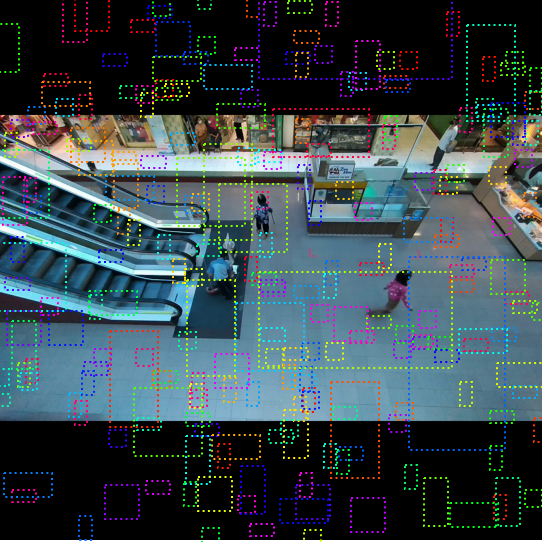
\includegraphics[width= 0.45\linewidth]{bab4/Anchor Box Negative.png}
    \caption{Contoh Hasil \textit{Anchor Box} yang Tidak Digunakan}
    \label{fig: Anchor Box Negative}
  \end{center}
\end{figure}

\subsection{Hasil Prediksi RPN dan Pembuatan \textit{Feature Map}}
Setelah jaringan \textit{residual network} dilatih menggunakan target RPN, maka prediksi RPN pun dapat dilakukan
oleh ResNet. Prediksi RPN dilakukan dengan menggunakan \textit{train-set} dan \textit{val-set} sehingga performa
model dapat diketahui secara lebih dalam terutama dalam mengidentifikasi adanya \textit{overfitting} maupun
\textit{underfitting}. RPN ini juga akan turut serta membantu dalam membentuk \textit{feature map} karena
jaringan ResNet ingin memperlihatkan fitur-fitur pada \textit{regional proposal network} yang telah diprediksi
dengan konvolusi dan \textit{pooling}. Pada tahap ini, RPN juga mendeteksi kelas pada objek di dalam \textit{bounding box}
namun deteksi kelas yang dimaksud ialah deteksi apakah objek tersebut termasuk \textit{foreground} atau 
\textit{background}. Dalam memprediksi kelas objek, \textit{loss} yang terjadi pada rpn umumnya bernilai
kecil karena hanya memprediksi dua nilai saja yaitu \textit{foreground} atau \textit{background}.

\begin{figure}[h!]
  \begin{center}
    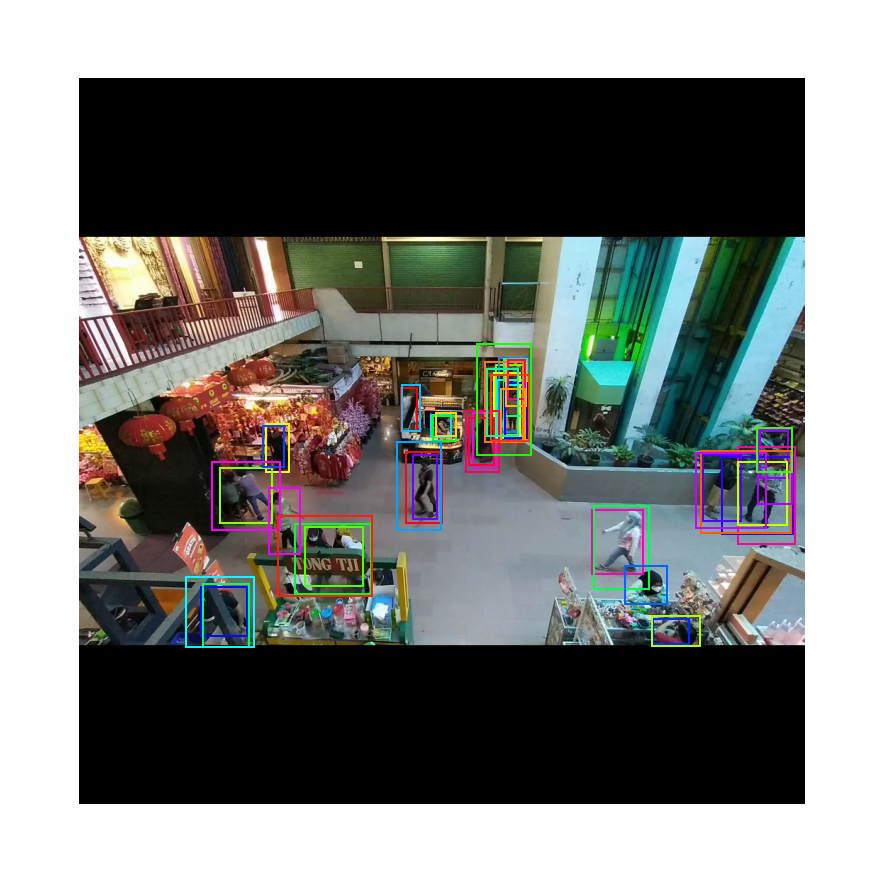
\includegraphics[width= 0.5\linewidth]{bab4/Prediksi RPN.png}
    \caption{Contoh Hasil Prediksi RPN}
    \label{fig: Prediksi RPN}
  \end{center}
\end{figure}

\begin{figure}[h!]
  \begin{center}
    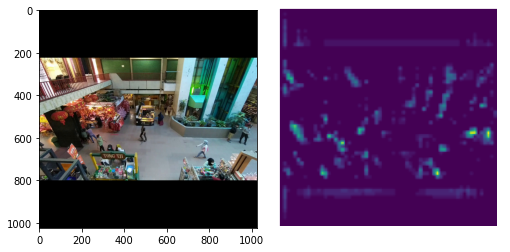
\includegraphics[width= 0.55\linewidth]{bab4/Feature Map Example.png}
    \caption{Contoh Hasil \textit{Feature Map}}
    \label{fig: Feature Map}
  \end{center}
\end{figure}

\subsection{Hasil \textit{Training}}
Pada bagian ini akan dijelaskan secara lebih mendalam mengenai hasil dari model yang telah dibentuk. 
Beberapa metriks \textit{loss} yang dipaparkan adalah sebagai berikut.

\begin{itemize}
  \item \textbf{\textit{Loss}} 
  
  Metriks \textit{loss} merupakan metriks yang menunjukkan jumlah dari segala \textit{loss} yang terjadi pada
  pemodelan, sedangkan \textit{val loss} adalah jumlah \textit{loss} yang terjadi saat model
  diuji coba pada dataset validasi.

  \item \textbf{\textit{RPN Bounding Box Loss}} 
  
  Metriks \textit{loss} mengenai \textit{bounding box} yang terjadi pada RPN menunjukkan adanya
  kesalahan prediksi pada jaringan \textit{backbone} dalam memprediksi \textit{bounding box} yang
  sesuai seperti target RPN. Kesalahan prediksi ditunjukkan dengan jauhnya jarak \textit{anchor box} asli
  dengan \textit{bounding box} yang diprediksi. Hasil \textit{RPN Bounding Box Loss} dari proses \textit{training} dapat dilihat pada gambar
  \ref{fig: RPN Bounding Box Loss Mask RCNN}.

  \item \textbf{\textit{RPN Class Loss}} 
  
  Sedangkan Metriks \textit{RPN Class loss} menunjukkan adanya kesalahan prediksi pada RPN
  untuk membedakan \textit{foreground} dan \textit{background} pada objek atau citra yang berada
  pada di dalam \textit{bounding box} yang telah diprediksi, nilai \textit{loss} ini umumnya bernilai
  lebih kecil daripada \textit{loss} yang lain karena hanya kesalahan prediksi untuk membedakan 
  dua kelas. Hasil \textit{RPN Class Loss} dari proses \textit{training} dapat dilihat pada gambar
  \ref{fig: RPN Class Loss}.

  \item \textbf{\textit{Mask RCNN Bounding Box Loss}} 
  
  Metriks \textit{Mask RCNN Bounding Box Loss} mengenai \textit{bounding box} yang terjadi pada 
  \textit{fully connected layer}. Hampir sama dengan metriks \textit{RPN Bounding Box Loss}, 
  kesalahan prediksi ditunjukkan dengan jauhnya jarak \textit{anchor box} asli
  dengan hasil akhir \textit{bounding box} yang diprediksi. Hasil \textit{Mask RCNN Bounding Box Loss} 
  dari proses \textit{training} dapat dilihat pada gambar \ref{fig: Bounding Box Loss Mask RCNN}.

  \item \textbf{\textit{Mask RCNN Class Loss}} 
  
  Metriks \textit{Mask RCNN Class Loss} memberikan penilaian mengenai kesalahan prediksi kelas,
  dimana pada penelitian ini, \textit{Mask RCNN Class Loss} akan bertambah jika Mask RCNN 
  memberikan kesalahan klasifikasi antara tiga kelas objek. Hasil \textit{Mask RCNN Class Loss} 
  dari proses \textit{training} dapat dilihat pada gambar \ref{fig: Class Loss Mask RCNN}.

  \item \textbf{\textit{Mask RCNN Mask Loss}}
  
  Metriks \textit{Mask RCNN Mask Loss} memberikan penilaian mengenai kesalahan pembentukan 
  \textit{mask} objek. Jika \textit{mask} yang dibentuk oleh model mempunyai selisih yang jauh dengan
  \textit{mask} yang dibentuk di awal, maka nilai \textit{Mask RCNN Mask Loss} akan bertambah.
  Hasil \textit{Mask RCNN Class Loss} dari proses \textit{training} dapat dilihat pada gambar 
  \ref{fig: Mask Loss Mask RCNN}.

\end{itemize}

Dalam pemilihan model terbaik yang dapat diaplikasikan, metriks \textit{val loss} merupakan yang
terbaik karena metriks tersebut mencerminkan bagaiman model Mask R-CNN bekerja pada data yang belum pernah
dilihat sebelumnya. Dari grafik-grafik \textit{loss} yang dipaparkan, dapat diperhatikan bahwa 
pada epoch 0 hingga 60, nilai \textit{loss} dan \textit{val loss} menunjukkan penurunan yang signifikan,
sedangkan pada epoch 60 hingga 150, nilai \textit{loss} tetap menurun, namun nilai \textit{val loss}
tidak menunjukkan adanya perubahan yang signifikan. Hal ini dapat dikarenakan kecilnya \textit{learning rate}
yang diaplikasikan atau karena model telah mencapai nilai optimal.
Nilai \textit{val loss} mencapai titik terendah pada epoch 124 dengan nilai 0,772 dan nilai 
\textit{loss} 0,5877. Karena nilai \textit{val loss} pada 
model epoch 124 mempunyai nilai terkecil, maka model inilah yang akan diteliti lebih lanjut dan diuji
coba pada test dataset. Namun sebelum itu, parameter \textit{loss} yang lain perlu dilihat untuk
memastikan apakah proses \textit{training} berjalan dengan baik. 

\begin{figure}[h!]
  \begin{center}
    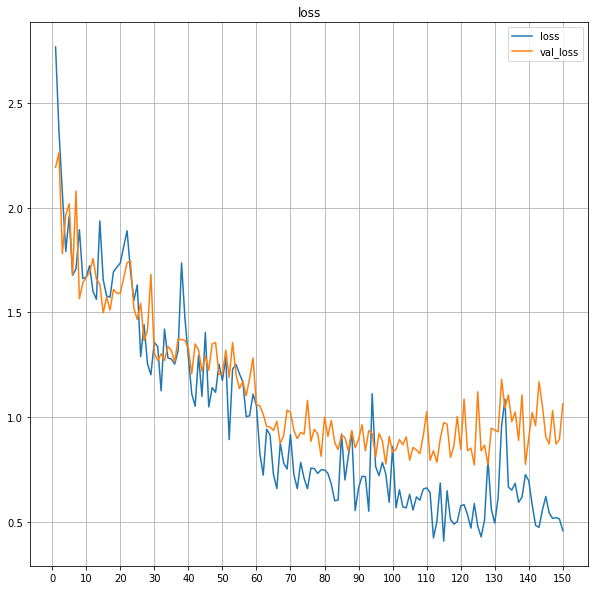
\includegraphics[width= 0.55\linewidth]{bab4/1. Loss_Result.png}
    \caption{Hasil \textit{Loss}}
    \label{fig: Loss}
  \end{center}
\end{figure}

Selain memberikan informasi mengenai nilai \textit{val loss} terendah, grafik \textit{loss} pada gambar \ref{fig: Loss} menunjukkan adanya \textit{overfitting}. \textit{Overfitting}
dapat diakibatkan oleh banyak faktor seperti arsitektur \textit{neural network}, penggunaan \textit{hyperparameter},
dan kurangnya dataset yang diambil. Dalam penelitian ini, kemungkinan besar hal ini terjadi karena adanya
ketidak seimbangan antara kelas dataset dan kurang dataset kelas \textit{crowd}. Karena itu \textit{overfitting}
terjadi, namun kualitas dari model dapat dilihat terlebih dahulu sehingga dapat diketahui apakah data
yang lebih banyak memang diperlukan, atau performa model dapat diterima walau mengalami \textit{overfitting}.
Selain itu komponen parameter \textit{loss} apakah yang menyebabkan nilai \textit{val loss} tidak mengalami penurunan
juga dapat diketahui jika melihat grafik setiap parameter \textit{loss}.

Selanjutnya pada metriks \textit{RPN Class Loss} (gambar \ref{fig: RPN Class Loss}) dapat dilihat bahwa
nilai \textit{loss} yang terjadi di awal sudah kecil dibandingkan metriks \textit{loss} yang lain. Nilai
awal pada \textit{RPN class loss} adalah 0,07 kemudian mempunyai nilai pada epoch 124 dengan nilai 0,0069.
Sehingga dapat dikatakan bahwa model pada epoch 124 dapat membedakan objek yang menjadi fokus (\textit{foreground})
dan objek yang menjadi latar belakang atau \textit{background}. Proses pembelajaran \textit{ResNet} dalam
membedakan \textit{foreground} maupun \textit{background} dapat terbilang cukup baik karena memiliki
nilai \textit{loss} yang menurun pada epoch 0 hingga 100, namun nilai \textit{loss} mulai berangsur naik
saat epoch lebih dari 100. Di saat inilah \textit{overfitting} mengenai prediksi \textit{foreground} dan
\textit{background} terjadi.

\begin{figure}[h!]
  \begin{center}
    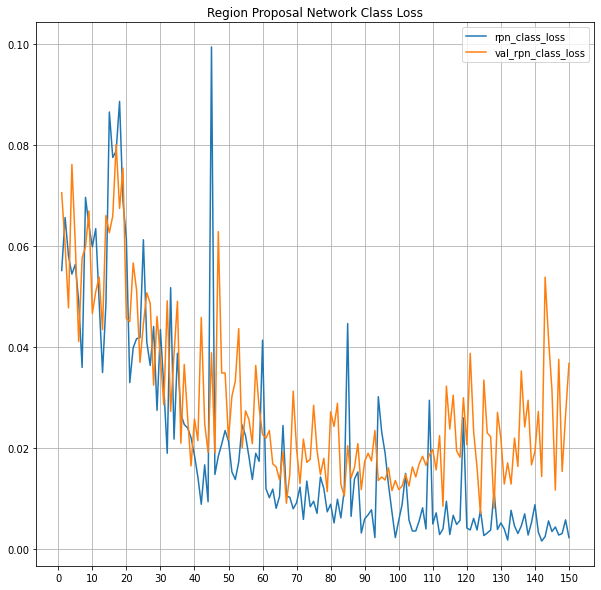
\includegraphics[width= 0.55\linewidth]{bab4/5. RPN_Class_Loss.png}
    \caption{Hasil \textit{Class Loss} RPN}
    \label{fig: RPN Class Loss}
  \end{center}
\end{figure}

Kemudian pada metriks \textit{RPN Bounding Box Loss} (gambar \ref{fig: RPN Bounding Box Loss Mask RCNN})
dapat dilihat bahwa nilai awal pada metriks \textit{loss} adalah 0,45 dan mencapai nilai minimal 0,1591
pada epoch 95. Sedangkan pada epoch 124 yang merupakan model dengan total val loss paling rendah memiliki \textit{val rpn bounding box loss} adalah 0,1921. 
Walaupun bukan nilai terendah, namun selisih nilai \textit{val rpn bounding box loss} epoch 124 mempunyai selisih
yang cukup kecil dengan epoch 95.

\begin{figure}[h!]
  \begin{center}
    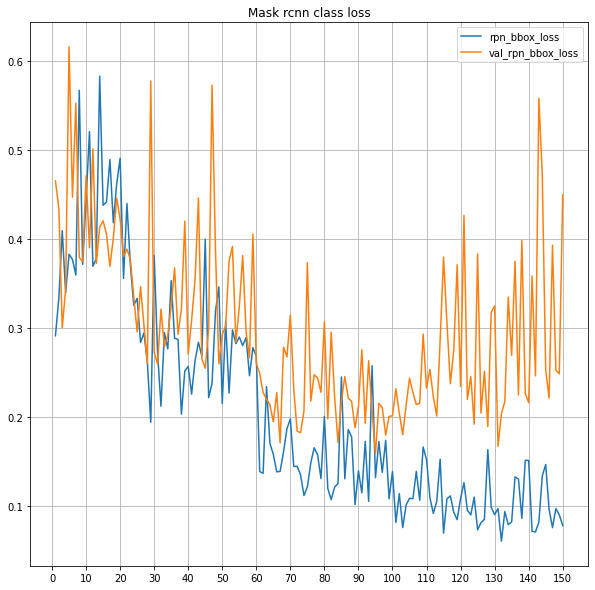
\includegraphics[width= 0.55\linewidth]{bab4/6. RPN_Bbox_Loss.png}
    \caption{Hasil \textit{Bounding Box Loss} RPN}
    \label{fig: RPN Bounding Box Loss Mask RCNN}
  \end{center}
\end{figure}

Selanjutnya pada metriks \textit{class loss Mask RCNN} (gambar \ref{fig: Class Loss Mask RCNN})
dapat dilihat bahwa nilai awal pada metriks \textit{val loss} berada di sekitar 0,7 dan mencapai nilai minimal 0,1032
pada epoch 144. Metriks \textit{class loss Mask RCNN} merupakan parameter yang menunjukkan apakah
Mask R-CNN dapat memprediksi kelas objek dengan benar atau tidak. Dalam melatih kemampuan Mask R-CNN
dalam mendeteksi kelas objek, dapat dilihat bahwa nilai loss kelas memiliki trend yang menurun. Seperti
metriks loss lainnya, pada epoch 0 hingga 60, penurunan nilai loss dapat dianggap drastis kemudian
dengan learning rate yang lebih kecil, penurunan nilai loss juga semakin kecil.

\begin{figure}[h!]
  \begin{center}
    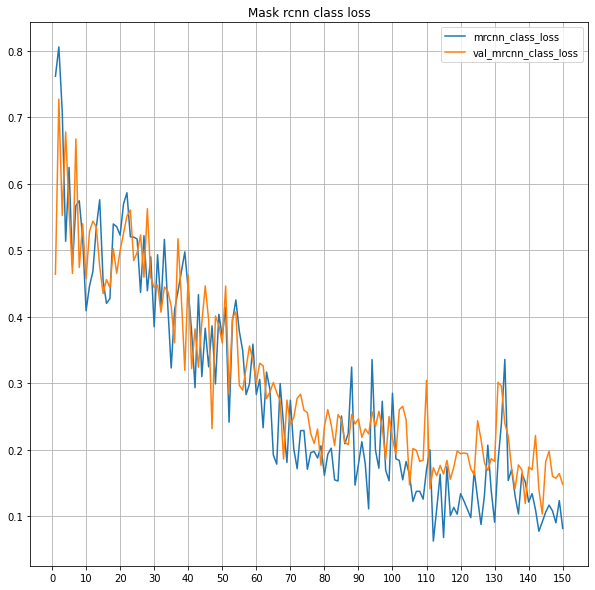
\includegraphics[width= 0.55\linewidth]{bab4/2. MRCNN_Class_Loss.png}
    \caption{Hasil \textit{Class Loss} Mask RCNN}
    \label{fig: Class Loss Mask RCNN}
  \end{center}
\end{figure}

Sedangkan pada metriks \textit{Loss Bounding Box Mask R-CNN} (gambar \ref{fig: Bounding Box Loss Mask RCNN})
awalnya memiliki nilai loss 0,63 namun perlahan lahan turun mendekati nilai stabil pada 0,17 setelah 
60 epoch. Parameter loss ini memiliki nilai terendah pada epoch 111 dengan nilai 0,1528. Tanda-tanda
\textit{overfitting} juga mulai terlihat setelah epoch 100, walaupun begitu nilai selisih antara loss
\textit{train} dan \textit{validation} tidak terlalu jauh hanya sekitar 0,05.

\begin{figure}[h!]
  \begin{center}
    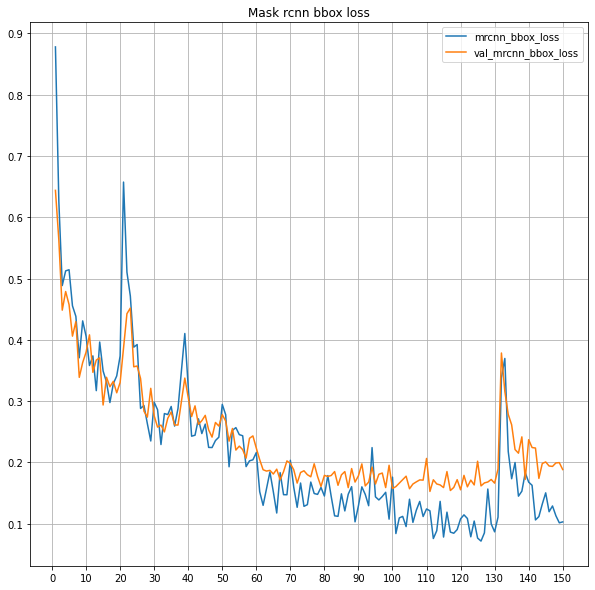
\includegraphics[width= 0.55\linewidth]{bab4/4. MRCNN_Bbox_Loss.png}
    \caption{Hasil \textit{Bounding Box Loss} Mask RCNN}
    \label{fig: Bounding Box Loss Mask RCNN}
  \end{center}
\end{figure}

Terakhir, metriks \textit{Loss Mask} digambarkan pada (gambar \ref{fig: Mask Loss Mask RCNN}).
Parameter ini merupakan parameter yang tercepat mencapai nilai stabil. Namun parameter loss ini memiliki
loss yang paling tinggi. Hal ini dikarenakan pembuatan mask diharapkan seakurat piksel segmentasi dataset,
namun untuk melakukan segmentasi secara akurat pada dataset pun merupakan hal yang sangat sulit dilakukan.
Nilai loss yang besar ini dapat memberikan masalah jika mask yang dibentuk sangat tidak sesuai dengan objek,
karena itu pengujian dengan test dataset sangat diperlukan untuk melihat performa model secara keseluruhan.

\begin{figure}[h!]
  \begin{center}
    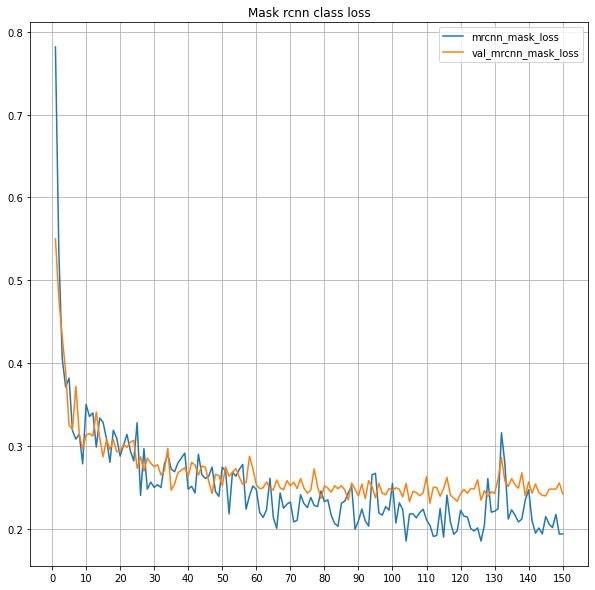
\includegraphics[width= 0.55\linewidth]{bab4/3. MRCNN_Mask_Loss.png}
    \caption{Hasil \textit{Mask Loss} Mask RCNN}
    \label{fig: Mask Loss Mask RCNN}
  \end{center}
\end{figure}

Berdasarkan parameter loss yang telah dipaparkan, maka peneliti memutuskan untuk mengambil model pada
epoch 124 karena memiliki nilai \textit{validation loss} terendah dari proses pelatihan. Model
pada epoch 124 memiliki detail \textit{loss} sebagai berikut.

\begin{table}
  \caption{Metriks Loss pada Model 124}
  \label{tab:MaskRCCN_Loss}
  \centering
  \begin{tabular}{ | l | l | }
    \hline
    \textbf{Parameter Model 124} & \textbf{Nilai} \\ \hline
    \textit{loss}             & 0,5877                   \\ \hline
    \textit{rpn class loss}    & 0,0076               \\ \hline
    \textit{rpn bounding box loss}             & 0,1102                  \\ \hline
    \textit{mrcnn class loss}             & 0,1683                   \\ \hline
    \textit{mrcnn bounding box loss}    & 0,1045                \\ \hline
    \textit{mrcnn mask loss}             & 0,1971                   \\ \hline

    \textit{val loss}             & 0,772                   \\ \hline
    \textit{val rpn class loss}    & 0,0069               \\ \hline
    \textit{val rpn bounding box loss}             & 0,1921                  \\ \hline
    \textit{val mrcnn class loss}             & 0,1620                   \\ \hline
    \textit{val mrcnn bounding box loss}    & 0,1634                \\ \hline
    \textit{val mrcnn mask loss}             & 0,2476                  \\ \hline
  \end{tabular}
\end{table}

\subsection{Hasil Pengujian pada Test Dataset}
Pengujian pada model epoch ke 124, dilakukan menggunakan test dataset yang mempunyai 134 gambar. Namun
sebelum model diuji secara keseluruhan, model akan diuji pada beberapa gambar. Hal ini dilakukan jika
hasil pada pengujian pada beberapa gambar menunjukkan nilai yang buruk, maka model tidak perlu diuji
dengan keseluruhan gambar.

\begin{figure}[h!]
  \begin{center}
    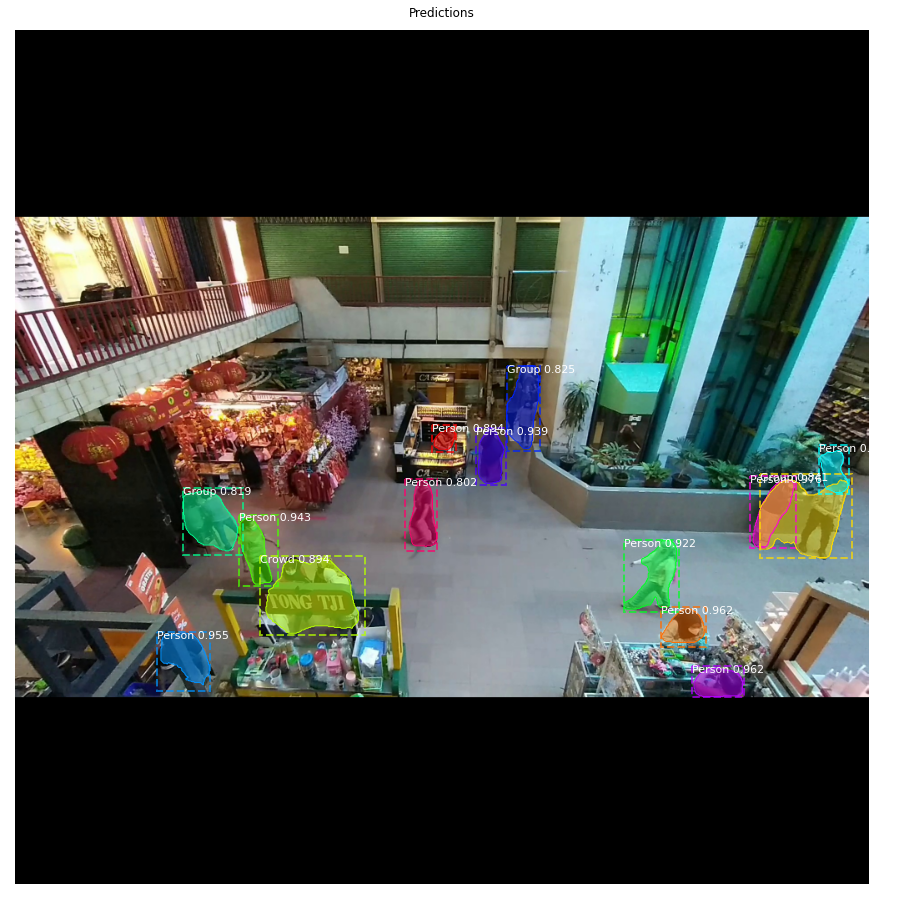
\includegraphics[width= 0.675\linewidth]{bab4/Contoh Hasil prediksi 1.png}
    \caption{Hasil Prediksi (1)}
    \label{fig: Predictions 1}
  \end{center}
\end{figure}

\begin{figure}[h!]
  \begin{center}
    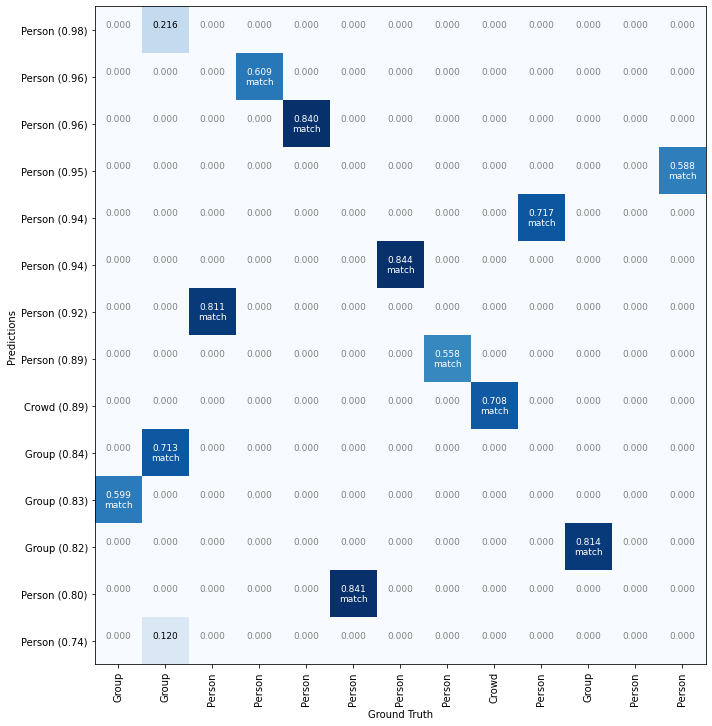
\includegraphics[width= 0.675\linewidth]{bab4/Contoh Hasil prediksi 1.6.png}
    \caption{Hasil Prediksi dan IoU (1)}
    \label{fig: Predictions and IoU}
  \end{center}
\end{figure}

\begin{figure}[h!]
  \begin{center}
    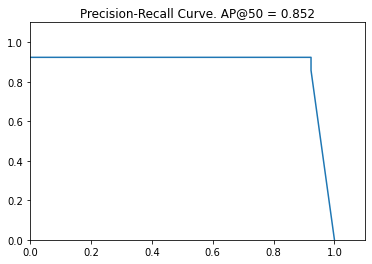
\includegraphics[width= 0.55\linewidth]{bab4/Contoh Hasil prediksi 1.5.png}
    \caption{Hasil Kurva Prediksi dan Recall (1)}
    \label{fig: line Predictions and IoU}
  \end{center}
\end{figure}

Gambar \ref{fig: Predictions and IoU} menunjukkan objek yang diprediksi dan \textit{ground truth} dimana
nilai prediksi dianggap benar jika IoU diatas 0,5. Dapat dilihat bahwa pada pengujian ini, 12 dari 14 objek
dapat diprediksi secara benar dan dengan \textit{confidence} di atas 70\%. Nilai \textit{confidence}
dapat dilihat pada label sebelah kiri, sebagai contoh Person(0,96) berarti, model yang diaplikasikan
mendeteksi suatu objek dengan nilai \textit{confidence} 96\% bahwa objek tersebut adalah objek kelas person.
Sedangkan nilai yang berwarna biru adalah nilai dari \textit{intersect over union} dimana jika nilai 
tersebut berada di atas nilai 0,5 maka dianggap prediksi benar.

Sedangkan grafik pada gambar \ref{fig: line Predictions and IoU} menunjukkan grafik hubungan antara
presisi dan \textit{recall} pada gambar yang diprediksi. Nilai pada x-axis menunjukkan nilai \textit{recall}
sedangkan nilai pada y-axis menunjukkan nilai presisi dan nilai \textit{threshold}. Gambar \ref{fig: line Predictions and IoU}
menunjukkan bahwa, saat diuji coba pada gambar tersebut, dengan threshold deteksi (\textit{confidence})
0,852, nilai presisinya ialah 0,852 dan nilai \textit{recall} adalah 0,92. Model ini dapat dikatakan model
yang bagus dalam mendeteksi gambar tersebut.

Kemudian saat diuji coba dengan gambar kedua, dapat dilihat bahwa model mendeteksi objek pada gambar
dengan baik. dengan \textit{threshold} 0,812, nilai presisi dan \textit{recall} pada model pun cukup
bagus. Deteksi yang dihasilkan pada uji coba gambar kedua ini pun dapat dihitung cukup memuaskan 
karena nilai \textit{confidence} di atas nilai 0,8. Walaupun ada satu objek kelas\textit{group} yang 
tidak terdeteksi, namun dari 8 objek yang ada, model dapat mendeteksi 7 objek dengan kelas yang benar
dan mayoritas objek yang dideteksi mempunyai nilai \textit{interference over union} di atas 0,7. terdapat
satu objek kelas yang memiliki \textit{interference over union} 0,693, namun saat dilihat pada gambar,
objek tersebut memiliki \textit{mask} yang cukup baik. Kemudian dapat dilihat juga bahwa model
dapat memprediksi objek \textit{person} yang hanya terlihat bagian kakinya, tentunya ini dapat dinilai
sebagai model yang cukup cerdas dalam memperhatikan fitur manusia. Hasil prediksi pada gambar
kedua dapat dilihat pada gambar \ref{fig: Predictions 2}. Sedangkan untuk nilai \textit{confidence} dan
nilai IoU dapat dilihat pada gambar \ref{fig: Predictions 2.6} dan kurva \textit{precission-recall} dapat 
dilihat pada gambar \ref{fig: Predictions 2.5}. Dengan hasil ini dapat disimpulkan secara sementara
bahwa model yang dibentuk memiliki kemampuan deteksi yang baik.

\begin{figure}[h!]
  \begin{center}
    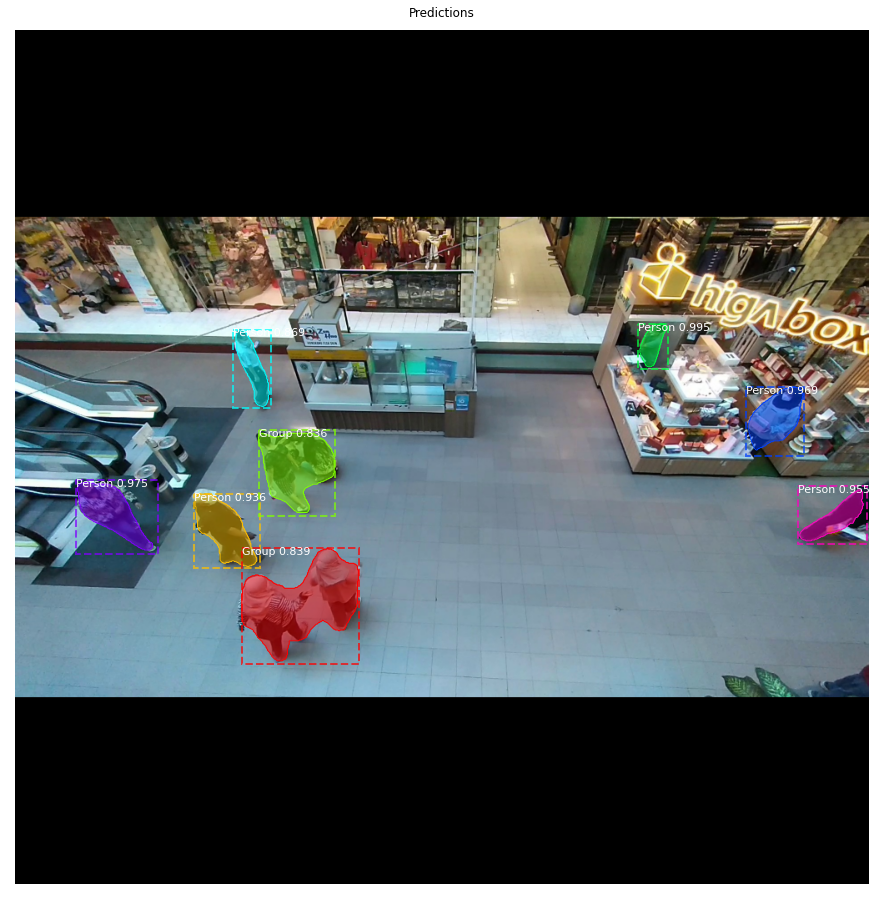
\includegraphics[width= 0.7\linewidth]{bab4/Contoh Hasil prediksi 3.png}
    \caption{Contoh Hasil Prediksi (2)}
    \label{fig: Predictions 2}
  \end{center}
\end{figure}

\begin{figure}[h!]
  \begin{center}
    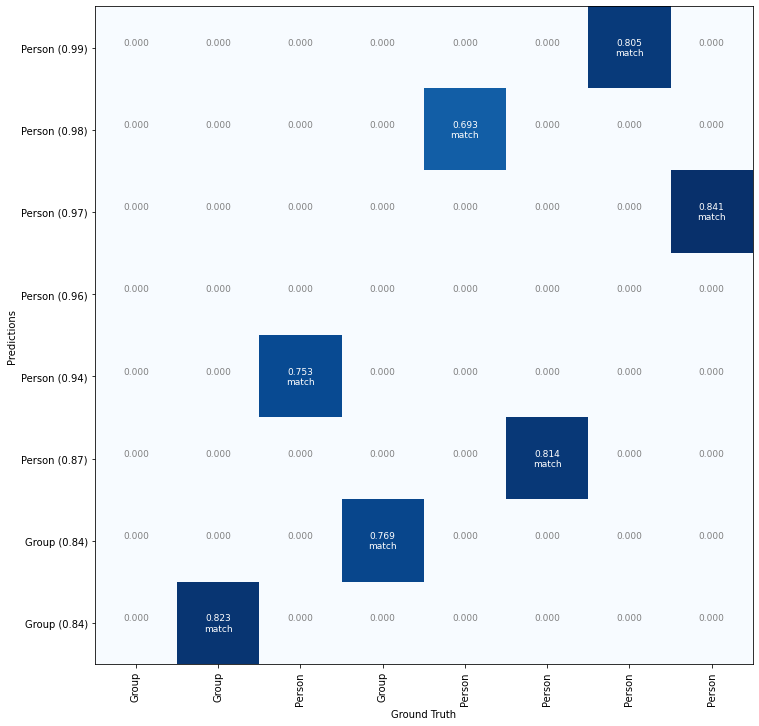
\includegraphics[width= 0.7\linewidth]{bab4/Contoh Hasil prediksi 3.6.png}
    \caption{Hasil Kurva Prediksi dan Recall (2)}
    \label{fig: Predictions 2.6}
  \end{center}
\end{figure}

\begin{figure}[h!]
  \begin{center}
    \includegraphics[width= 0.7\linewidth]{bab4/Contoh Hasil prediksi 3.5.png}
    \caption{Contoh Hasil Prediksi dan IoU(2)}
    \label{fig: Predictions 2.5}
  \end{center}
\end{figure}

\begin{figure}[h!]
  \begin{center}
    \includegraphics[width= 0.55\linewidth]{bab4/Hasil Test.png}
    \caption{Beberapa Hasil Deteksi pada Dataset Test}
    \label{fig: Test Dataset Result}
  \end{center}
\end{figure}

Setelah pengujian dengan beberapa gambar, maka pengujian dilakukan menggunakan seluruh test dataset.
Hasil dari pengujian divisualisasikan dengan \textit{confusion matrix} pada gambar \ref{fig: Conf Matrix Test}.
Perlu diketahui bahwa parameter deteksi adalah dimana model memiliki \textit{confidence} lebih dari 
70\% pada sebuah deteksi objek dan memiliki \textit{interference over union} lebih dari 50\%. Pada
\textit{confusion matrix} kita dapat mengetahui bahwa akurasi secara menyeluruh dari model yang dihasilkan adalah 88,79\%. 
Dari total 591 objek kelas \textit{person}, model dapat mendeteksi 531 objek kelas person yang benar.
Sedangkan dari total 296 objek dengan kelas \textit{group}, model dapat mendeteksi 261 objek kelas 
\textit{group} secara benar. Terakhir, dari total 32 objek kelas \textit{crowd}, terdapat 24 objek
kelas \textit{crowd} yang dideteksi dengan benar. Selain itu, tidak ada satupun objek dengan kelas 
\textit{person} dideteksi sebagai objek kelas \textit{crowd}

Dapat dilihat juga bahwa \textit{recall} pada objek kelas \textit{person} adalah 89,85\% dan memiliki
presisi sebesar 95,85\%. Selanjutnya pada objek kelas \textit{group}, \textit{recall} yang dihasilkan
adalah 88,17\% dengan presisi sebesar 79,33\%. Terakhir pada objek kelas \textit{crowd}, model memiliki
performa deteksi yang paling rendah dibandingkan kelas yang lainnya yaitu 75\% \textit{recall} dan
66,67\% pada presisi. Namun semua kelas \textit{crowd} terdeteksi sebagai kelas \textit{crowd} dan
\textit{group}. Tidak ada kelas \textit{crowd} yang terdeteksi sebagai kelas \textit{person} sehingga
kelas ini dapat dianggap sebagai terdeteksi sebagai parameter yang berbahaya dalam masa pandemi Covid-19.

\begin{figure}[h!]
  \begin{center}
    \includegraphics[width= 0.5\linewidth]{bab4/Confusion Matrix.png}
    \caption{\textit{Confusion Matrix} dari Hasil Prediksi Test Dataset}
    \label{fig: Conf Matrix Test}
  \end{center}
\end{figure}

	\cleardoublepage
	\chapter{PENUTUP}
\label{sec:chap5_tutup}
\vspace{1ex}
\section*{}

\section{Kesimpulan}
\label{sec:sec4_kesimpulan}
\vspace{1ex}
Pada penelitian ini, sebuah dataset mengenai aktivitas jual beli pada suatu pusat perbelanjaan Di
Surabaya berhasil dibentuk dengan total gambar 730 dan total objek 4.980.
Dataset yang dibentuk memiliki total objek kelas \textit{person} sebanyak 3.382 objek,
objek kelas \textit{group} sebanyak 1.350 objek, dan objek kelas \textit{crowd} sebanyak 248 objek.
Dataset tersebut dapat diakses pada \href{https://www.kaggle.com/datasets/lukaspurbaw/indonesia-pasar-atom-crowd-dataset}. 
Selain dataset, penelitian ini juga memberikan kontribusi berupa alur kerja penerapan deteksi objek
kerumunan pada pusat perbelanjaan, dan memberikan model yang dapat mendeteksi kerumunan dengan baik.
Berdasarkan hasil penilitian ini penggunaan algoritma Mask R-CNN pada dataset ini terbukti dapat 
membedakan objek kelas \textit{person} dimana objek kelas \textit{person} adalah orang yang tidak berdekatan dengan orang lain
dalam jarak kurang lebih satu meter dengan objek kelas \textit{group} dan kelas \textit{crowd} yang
merupakan objek orang yang saling berdekatan dalam jarak satu meter.  Model Mask R-CNN yang dibentuk
dengan \textit{backbone} ResNet 101 memiliki akurasi 88,79\% dalam mendeteksi objek pada dataset dengan
parameter \textit{confidence} lebih dari sama dengan 70\% dan \textit{intersect over union}
lebih dari sama dengan 50\% dengan \textit{mask} asli meskipun terdapat ketidak seimbangan data. Model yang dibentuk masih memiliki nilai \textit{recall}
dan presisi yang kecil dalam mendeteksi objek kelas \textit{crowd} karena data kelas \textit{crowd}
hanyalah 5\% dari total seluruh objek yang ada. Secara umum, model yang dibentuk dapat memprediksi 
adanya \textit{group} dan \textit{crowd}. Namun apakah model ini dapat digunakan dalam tempat
pusat perbelanjaan lain masih perlu diteliti lebih lanjut.

\section{Saran}
\label{sec:sec4_saran}
\vspace{1ex}
Walaupun model ini secara umum sudah dapat mendeteksi apakah terdapat kerumunan atau tidak, namun
nilai \textit{recall} dan presisi saat mendeteksi objek \textit{crowd} masih dinilai rendah. Hal ini
disebabkan oleh tidak seimbangnya dataset yang telah dikumpulkan. Dikarenakan pengumpulan dataset
dilakukan pada masa pandemi Covid-19, maka jumlah kerumunan yang terjadi pun tidak banyak. Dataset
dan model dapat diperbaiki dengan menambah data terutama objek kelas \textit{crowd}.


	\cleardoublepage
	%Bab Lain bisa ditambah disini
\end{spacing}
\DaftarPustaka
%Daftar Riwayat Hidup
%    ->\ubah\DaftarRiwayatHidup.tex
\DaftarRiwayatHidup
\end{document}